% % % % % % % % % % % % % % % % % % % % % % % % % % % % % % % % 
% Thesis - Ian Huston
% $Id: thesis.tex,v 1.2 2009/12/17 18:16:48 ith Exp $
% % % % % % % % % % % % % % % % % % % % % % % % % % % % % % % %
%\pdfoutput=1

\documentclass[
%  twoside,
PhD, % Change to PhD to change text at bottom of title page
DIC=off,
12pt,
bibliography=totoc, % Include bibliography in contents
listof = totoc, % Include lists of figures and tables in contents
index= totoc, % Include index in contents
onehalfspacing, % onehalfspacing or doublespacing
a4paper %letterpaper
% doublespacing
%,openright
]
{icldt}

\usepackage{graphicx}

%\usepackage[square, numbers, sort&compress]{natbib}
\usepackage[]{natbib}
%\bibliographystyle{JHEP}
\bibliographystyle{mnras}

%%further packages:
\usepackage{amsmath,amssymb,amsfonts}
\usepackage{bm}
\usepackage[T1]{fontenc}

% % % % % % % % % % % % % % % % % % % % % % % % % % % % % % % % 

% Journals
% \newcommand{\apj}{ApJ}
% \newcommand{\apjs}{ApJS}
% \newcommand{\apjl}{ApJL}
% \newcommand{\aap}{A{\&}A}
% \newcommand{\aaps}{A{\&}AS}
% \newcommand{\mnras}{MNRAS}
% \newcommand{\aj}{AJ}
% \newcommand{\araa}{ARAA}
% \newcommand{\pasp}{PASP}
% \newcommand{\pasj}{PASJ}
% \newcommand{\jcap}{JCAP}
% \newcommand{\na}{New Astronomy}
% \newcommand{\physrep}{Phys. Rep.}
% \newcommand{\prd}{Phys. Rev. D}
% \newcommand{\azh}{Astron. Zh.}
% \newcommand{\nat}{Nature}
% \newcommand{\nar}{New Astronomy Reviews}

% % % % % % % % % % % % % % % % % % % % % % % % % % % % % % % % 
% IH formatting package
% CVSon for cvs revision number in footers
% CVSoff is default-
%\usepackage[%CVSon, % CVS version in footers
            %labels, % show labels
	        %todos, % show todos (requires todonotes package)
            %hyperref % Use hyperref for links
%            ]{ihformat}

\pagestyle{headings}
\usepackage{hyperref}
\usepackage[title]{appendix}
            
\hypersetup{colorlinks = true, linkcolor=blue}
            
%\usepackage[style=ieee-alphabetic]{biblatex}

% Redefine CVSRevision for this section
% \renewcommand{\CVSrevision}{\version$Id: thesis.tex,v 1.2 2009/12/17 18:16:48 ith Exp $}
% % % % % % % % % % % % % % % % % % % % % % % % % % % % % % % % 


% % % % % % % % % % % % % % % % % % % % % % % % % % % % % % % % 
% Include list
% Put in all the files that you want to compile each time.
% You must run with all the files added at least once to get the correct reference
% aux and toc files.
%\includeonly{
%abstract_corrected,
%acknowledgements,
%C1_Intro,
%C2_CPT,
%C3_History,
%C4_zeta2,
%C6_iso2,
%C5_quench,
%C7_palatini,
%C9_conclusions,
%AppendixA,
%AppendixB
%}

% % % % % % % % % % % % % % % % % % % % % % % % % % % % % % % % 
%dodgy addition...
\makeatletter
%% change \numberline so that it will print "Appendix A"
\newcommand\appendix@numberline[1]{}%\autodot\ } %#1} %\appendixname\  }
\g@addto@macro\appendix{%
  \addtocontents{toc}{
    \let\protect\numberline\protect\appendix@numberline}%
}
\makeatother
%end dodgy addition


%%%%%%%%%%%%%%%%%%%%%%%%%%%%%%%%%%%%%%%%%%%%%%%%%%%%%%%%%%%%%%%%%%% 
% % % custom commands 

%maths
\renewcommand{\mathbf}{\bm}
\newcommand{\n}{\bm {n}}
\renewcommand{\k}{\bm {k}}
\newcommand{\x}{\bm {x}}
\newcommand{\ka}{\bm {k}_1}
\newcommand{\kb}{\bm {k}_2}
\newcommand{\kc}{\bm {k}_3}
\newcommand{\ko}{\mathcal{K}}
\newcommand{\kt}{\mathcal{K}^{(2)}}
\newcommand{\ks}{\bm {k}_S}
\newcommand{\kl}{\bm {k}_L}
\newcommand{\ep}{\varepsilon}
\newcommand{\p}{\partial}
\newcommand{\cH}{\mathcal{H}}

\def\i{\mathrm{i\,}}


%%%%%%%%%%%%%%%%%%%%%%%%%%%%%%%%%%%%%%%%%%%%%%%%%%%%%%%%%%%%%%%%%%%

\begin{document}

% Title page is input not included to remove extra page.
\setlength{\tabcolsep}{0in}
\newcommand{\isep}{-2 pt}
\newcommand{\lsep}{-0.5cm}
\newcommand{\psep}{-0.6cm}
\renewcommand{\labelitemii}{$\circ$}
%


\college{Queen Mary, }
%
%
\department{Physics and Astronomy}
%
%
\supervisor{Dr Chris Clarkson}
%
%
%
\title{Relativistic effects in the galaxy bispectrum}
% \title{On the relativistic bispectrum of large scale structure}
%\title{BS about the BS}
%
%
\author{Eline Maaike de Weerd}
\date{17.12.2021}% cth added
%Note Actual title format is done in icldt.cls
%
%
%\hypersetup{pdftitle={Non-linear effects in early Universe cosmology},pdfauthor={Pedro Carrilho}}
%

% Change as appropriate
\declaration{%
I, Eline Maaike de Weerd, confirm that the research included within this thesis is my own work or that where it has been carried out in collaboration with, or supported by others, that this is duly acknowledged below and my contribution indicated. Previously published material is also acknowledged below.
\newline
\newline
I attest that I have exercised reasonable care to ensure that the work is original, and does not to the best of my knowledge break any UK law, infringe any third party's copyright or other Intellectual Property Right, or contain any confidential material.
\newline
\newline
I accept that the College has the right to use plagiarism detection software to check the electronic version of the thesis.
\newline
\newline
I confirm that this thesis has not been previously submitted for the award of a degree by this or any other university. The copyright of this thesis rests with the author and no quotation from it or information derived from it may be published without the prior written consent of the author.
\newline
\newline
Details of collaboration and publications:
Part of this work has been done in collaboration with Stefano Camera, Chris Clarkson, Sheean Jolicoeur, Roy Maartens, and Obinna Umeh. It is based on the following publications, all of which I have contributed to:
\begin{itemize}
	\item \underline{The dipole of the galaxy bispectrum} \\
	C. Clarkson, E.M. De Weerd, S. Jolicoeur, R. Maartens, O. Umeh \\
	Published: \textit{MNRAS Letters 486 (2019) L101},	arXiv: 1812.09512 [astro-ph.CO]
	\item \underline{Detecting the relativistic galaxy bispectrum} \\
	R. Maartens, S. Jolicoeur, O. Umeh, E.M. De Weerd, C. Clarkson, S. Camera\\
	Published: \textit{JCAP03(2020)065},	arXiv: 1911.02398 [astro-ph.CO]
	\item \underline{Multipoles of the relativistic galaxy bispectrum} \\
	E.M. De Weerd, C. Clarkson, S. Jolicoeur, R. Maartens, O. Umeh \\
	Published: \textit{JCAP05(2020)018},	arXiv: 1912.11016 [astro-ph.CO]
	\item \underline{Detecting the relativistic bispectrum in 21cm intensity maps} \\
	S. Jolicoeur, R. Maartens, E.M. De Weerd, O. Umeh, C. Clarkson, S. Camera \\
	Published: \textit{JCAP06(2021)039},	arXiv: 2009.06197 [astro-ph.CO]
	\item \underline{Local primordial non-Gaussianity in the relativistic galaxy bispectrum} \\
	R. Maartens, S. Jolicoeur, O. Umeh, E.M. De Weerd, C. Clarkson \\
	Published: \textit{JCAP04(2021)013},	arXiv: 2011.13660 [astro-ph.CO]
\end{itemize}
This work was supported by an STFC PhD studentship.
\vfill
\noindent Signature: 
\newline
Date: 17.12.2021}
\thispagestyle{empty}


\maketitle


% % % % % % % % % % % % % % % % % % % % % % % % % 
% Abstract
\chapter*{Abstract}
\label{ch:abstract}
\addcontentsline{toc}{chapter}{Abstract}
\section*{}
\singlespacing

% \thispagestyle{empty} if wanting to remove page numbering from abstract

Next-generation galaxy surveys will provide us with a wealth of high-precision cosmological data. To be able to use this information in an as unbiased manner as possible, theoretical accuracy must match the experimental precision. The three-point function, or bispectrum, is the first of the higher-order statistics beyond the power spectrum, and contains information both complementary and additional to what is contained in the power spectrum.

On large scales, the galaxy bispectrum will be a key probe for measuring primordial non-Gaussianity, improve constraints on cosmological parameters, and hence help discriminate between various models of inflation and other theories of the early universe. On these scales, a variety of relativistic effects come into play once the galaxy number-count fluctuation is projected onto the past light cone. It is important for these effects to be taken into account in our theoretical treatment of the bispectrum, as they will contaminate the primordial non-Gaussian signal and bias measurements. 

In this thesis, we review the relativistic projection effects in the galaxy bispectrum, and examine in detail how these relativistic effects contribute to the invariant multipoles of the galaxy bispectrum about the observer's line of sight. The Fourier-space bispectrum is complex, with an imaginary part arising from the relativistic effects only, which generates odd multipoles. This means that detection of this imaginary part is a smoking gun signal of the relativistic contributions, and we show that such a signal is in principle detectable in future surveys, although with a higher signal-to-noise ratio for spectroscopic surveys compared to 21cm intensity mapping surveys. Finally, we include local primordial non-Gaussianity in the theoretical description of the relativistic galaxy bispectrum. This allows for more precise separation of the relativistic corrections from the primordial signal.

\iffalse
Finally, we include local primordial non-Gaussianity in the theoretical description of the relativistic bispectrum, separating the relativistic corrections from the primordial signal, and use the bispectrum in Fisher matrix forecasts for cosmological parameters.
\fi

% % % % % % % % % % % % % % % % % % % % % % % % %

% % % % % % % % % % % % % % % % % % % % % % % % % 
% Acknowledgements
\chapter*{Acknowledgements}
\label{ch:acknowledgements}
\addcontentsline{toc}{chapter}{Acknowledgements}

\todo{Acknowledgements}Round up the usual suspects
% % % % % % % % % % % % % % % % % % % % % % % % % 


% % % % % % % % % % % % % % % % % % % % % % % % % 
% Table of contents and figures
% % % % % % % % % % % % % % % % % % % % % % % % % 
\tableofcontents

% Set one half spacing now that thesis proper is starting.
\onehalfspacing
% % % % % % % % % % % % % % % % % % % % % % % % % 

% Include files for each chapter here using 
\chapter{The Dipole of the Galaxy Bispectrum}
\label{chapter:dipole}

\section{The dipole}

\iffalse
The bispectrum will be crucial in next-generation large scale structure surveys, as it contains information that is both complementary and additional to what is contained in the power spectrum. As a non-Gaussian statistic it is well-suited to detect and constrain primordial non-Gaussianity, a key goal of next-generation surveys, and hence can help discriminate between various theories of inflation and other theories of the early universe.

On cosmological scales, observations on the past light-cone induce relativistic corrections to the observed bispectrum of galaxies. As theoretical accuracy must at least match experimental precision, it is crucial for these effects to be included in the analysis of the Fourier-space bispectrum. The inclusion of redshift-space distortions (RSD) in the bispectrum is therefore essential~\citep{Verde:1998zr,Scoccimarro:1999ed}. This will add complexity, but means that more information can potentially be extracted~\citep{Tellarini:2016sgp}.
\fi

In this chapter we examine the leading-order relativistic contributions in the galaxy bispectrum, which arise predominantly from RSD and other Doppler-type observational effects. These give rise to corrections at $\ord(\cH/k)$ in the galaxy bispectrum. Higher order $\cH/k$ contributions are, while being subdominant, still present in the galaxy bispectrum; and a full treatment of the bispectrum at all orders can be found in chapter~\ref{chapter:multipoles}.


\todo{remove this fluff, move to intro} The dominant RSD effect on galaxy number counts at first order is given by $\delta_g(z,\k) = (b_{1}(z) + f (z) \mu^{2})\delta(z,\k)$, where $\mu=\n\cdot\hat{\k}$, with $\n$ the line of sight direction, $f$ the growth rate, and $b_1$ is the linear bias. Henceforth the redshift dependence will be dropped for brevity as we are working at fixed redshift. At leading order, there is a Doppler type correction to this effect~\citep{Kaiser:1987qv,McDonald:2009dh,Challinor:2011bk} (see also \citep{Raccanelli:2016avd,Hall:2016bmm,Abramo:2017xnp}) proportional to $\bm{v}\cdot\n$, where $\bm{v}$ is the peculiar velocity:\footnote{\citep{Challinor:2011bk} provides the relativistic correction to the coefficient of  $\bm{v}\cdot\n$ given in \citep{Kaiser:1987qv,McDonald:2009dh}.}
\begin{equation} \label{dopf}
\delta_g(\x) = b_{1} \delta(\x)-{\frac{1}{\cH}}\partial_r(\bm{v}\cdot\n) +{A}\,\bm{v}\cdot\n ~~\to~~
\end{equation}
\begin{equation} \delta_g(\k)=\Big(b_1+f\mu^2+\i {A}\,f \mu{\frac{\cH}{k}}\Big)\delta(\k)\,,\label{dopf2}
\end{equation}
where  
\begin{equation}
{A} = {b_{\textrm{e}}+{3}\Omega_m/2 -3 + (2-5s) (1-{1/ r\cH} )}\,.
\end{equation}
Here $b_{\textrm{e}}=\partial (a^3 \bar{n}_g)/\partial \ln a$ is the evolution of comoving galaxy number density, $s=-(2/5)\partial \ln \bar{n}_g/\partial \ln L$ is the magnification bias ($L$ is the threshold luminosity), $r$ is the comoving radial distance ($\partial_r=\bm n\cdot\bm\nabla$) and we have assumed a $\Lambda$CDM background ($\cH'/\cH^2=1-3\Omega_m/2$, where $\cH$ is the conformal Hubble rate, a prime is differentiation with respect to conformal time, $\Omega_m$ is the evolving density contrast). In the  Fourier space expression~\eqref{dopf2} we can read off the relative contribution of each term by how they scale with $k$: terms like $\cH/k$ are suppressed on small scales when $\cH/k\ll1$ but become important around and above the equality scale. 


Although the galaxy density contrast~\eqref{dopf2} is complex, the power spectrum of a single tracer is real:
\begin{equation}
\big\langle \delta_g(\k)\delta_g(-\k)\big\rangle
=\Big[ \big(b_{1} + f\mu^{2}\big)^2+\Big(A\,f \mu \frac{\cH}{k}\Big)^2\Big] \big\langle \delta(\k)\delta(-\k)\big\rangle \,,\nonumber
\end{equation}
since $\mu_{-\k}=-\mu_{\k}$ enforces a cancellation of the imaginary part, and the RSD contribution is separate from the Doppler term.
However, if we consider the cross-power spectrum for {\em two} matter tracers, this cancellation breaks down, and  there is an imaginary part in the cross-power~\citep{McDonald:2009dh,Bonvin:2014owa},
\begin{align}
P_{g \tilde g}(k)&= \Big\{\Big[ \big(b_{1} + f\mu^{2}\big)\big(\tilde b_{1} + f\mu^{2}\big)+A\tilde A f^2\mu^2 {\frac{\cH^2}{k^2}}\Big]\nonumber\\
&
+\i f\mu\Big[\big(\tilde b_{1} + f\mu^{2}\big)A-\big(b_{1} + f\mu^{2}\big)\tilde A\Big]{\frac{\cH}{k}} \Big\}P(k) \,.\nonumber
\end{align}
While the Doppler contribution to $P_g$ is $\ord((\cH/k)^{2})$,  the Doppler contribution to $P_{g\tilde g}$ mixes with the density and RSD to give an additional less suppressed part, i.e. $\ord(\cH/k)$. The nonzero multipoles of $P_g$ are $\ell=0,2,4$, whereas  $P_{g \tilde g}$ has a nonzero dipole (as well as a smaller octupole).  There are also further relativistic corrections to this dipole part of the cross power spectrum~\citep{DiDio:2018zmk}.


A natural question is: what about the galaxy bispectrum? In the standard `Newtonian' approximation, with only RSD, the galaxy bispectrum for a single tracer at fixed redshift has no dipole, and only has even multipoles~\citep{Scoccimarro:1999ed,Nan:2017oaq}. But
with a lightcone corrected galaxy density contrast, the 3-point correlator, even for a {\em single} tracer, will no longer be an even function of $\k_a\!\cdot\n \,(a=1,2,3)$. In order to compute the consequent contribution to the galaxy bispectrum, \eqref{dopf} is not sufficient: we need its second-order generalisation, $\delta_g \to \delta_g+\delta^{(2)}_g/2$.

% \section{Relativistic contributions to the galaxy bispectrum}

At second order, the Doppler correction in~\eqref{dopf} generalises to $A\, \bm{v}^{(2)}\!\cdot\n$, but there are also quadratic coupling terms. The couplings involve not only the Doppler effect, but also radial gradients of the potential (`gravitational redshift'), volume distortion effects, and second-order corrections to the density contrast. Most of these contributions are small, but those that scale as $(\cH/k)\delta^2$ are not, even on equality scales. Except on super-equality scales we can often neglect any terms $\ord((\cH/k)^{2})$ and higher, which makes the calculation considerably simpler. The treatment of higher-order terms is left to chapter~\ref{chapter:multipoles}.

The leading correction can be extracted from the general expressions that include all relativistic  corrections to the Newtonian approximation, as given in~\citet{Bertacca:2014hwa} (see also~\citet{Bertacca:2014dra,Yoo:2014sfa,DiDio:2014lka,Jolicoeur:2017nyt,DiDio:2018zmk}), 
\begin{align}
\delta^{(2)}_{g{\mathrm{D}}} &= A \, \bm{v}^{(2)}\!\!\cdot\n+2{C}(\bm{v}\cdot\n)\delta +2 {\frac{E}{\cH}}(\bm{v}\cdot\n)\partial_r(\bm{v}\cdot\n)\label{dg2}
\\ & \nonumber
+ 2 \frac{b_1}{\cH}\phi\, \partial_r\delta
+ \frac{2}{\cH^2} \big[\bm{v}\cdot\n \,\partial_r^2\phi-\phi\, \partial_r^2 (\bm{v}\cdot\n) \big] - \frac{2}{\cH}\partial_r (\bm{v}\cdot\bm{v}), 
\end{align}
where $\phi$ is the gravitational potential, and the coefficients C and E are,
\begin{equation}
    C = b_1(A + f)+{b_1'/ \cH}+ 2(1-{1/ r\cH} ){\partial b_1/ \partial\ln L}\,,
\end{equation}
and
\begin{equation}
E = {4-2A-{\frac{3}{2}}\Omega_m}\,.
\end{equation}
This is in agreement with the independent re-derivation of the leading correction given in~\citet{DiDio:2018zmk}. We have corrected a typo in the last bracket of line 1 of Eq. (2.15): $-f_{\mathrm{evo}}\to -2f_{\mathrm{evo}}\equiv -2b_{\mathrm{e}}$. Note that our $\n$ is minus theirs, and they use the convention $\delta_g+\delta^{(2)}_g$.
All but one of the contributions to this leading term contain Doppler contributions, so we label these terms with a D subscript. In this sense, they can be thought of as the relativistic correction to redshift space distortions, but their origin is considerably more subtle than in the Newtonian picture~\citep{Bertacca:2014dra,DiDio:2018zmk}. These relativistic corrections all arise as projections along the line of sight $\n$. It is this projection that is responsible for the dipole in the observed bispectrum. Beyond these leading terms in~\eqref{dg2} there are a host of local coupled terms which appear on larger scales. 

We follow most work on the Fourier bispectrum and neglect the effect of lensing magnification. This is reasonable for correlations at the same redshift and when using very thin redshift bins allowed by spectroscopic surveys~\citep{DiDio:2018unb}. We also use the standard plane-parallel approximation, which is reasonable on ultra-large scales. However, we note that wide-angle effects in the power spectrum can be of the same order of magnitude as the Doppler-type effects in certain circumstances~\citep{Tansella:2017rpi}, and these should be incorporated in a more complete treatment.


The galaxy bispectrum is defined in Fourier space by,
\begin{align}
B_{g}( \mathbf{k}_{1},  \mathbf{k}_{2},  \k_3) &= { \mathcal{K}( \k_{1})\mathcal{K}({\k}_{2}) \mathcal{K}^{(2)}(  \mathbf{k}_{1},  \mathbf{k}_{2}, \k_3)}
P(k_{1})P(k_{2}) \nonumber\\ 
&+\text{2 cyclic permutations}\,.\label{eq:fsbispdef}
\end{align}
The first-order kernel $\mathcal{K}=\mathcal{K}_{\mathrm{N}}+\mathcal{K}_{\mathrm{D}}$ is given by the term in brackets in~\eqref{dopf2}.
At second order, $\mathcal{K}^{(2)}=\mathcal{K}_{\mathrm{N}}^{(2)}+\mathcal{K}_{\mathrm{D}}^{(2)}$, where
 the Newtonian kernel is~\citep{Verde:1998zr}
\begin{align}
\mathcal{K}_{\mathrm{N}}^{(2)} (\ka,\kb,\kc) &= b_{2} + b_{1}F_{2}(\ka,\kb) + b_s S_{2}(\ka,\kb) \nonumber \\
& + f \mu_3^{2} G_{2}(\ka,\kb)
+ {\cal Z}_2(\ka,\kb)\,.   \label{kn2}  
\end{align}
Here $F_2(\ka,\kb)$ is the standard Newtonian mode-coupling kernel for $\Lambda$CDM~\citep{Villa:2015ppa}, 
\begin{equation}
    F_2(a,\ka,\kb) = 1 + \frac{F(a)}{D(a)^2} + \left( \frac{k_1}{k_2} + \frac{k_2}{k_1} \right) \hat{\k}_1 \cdot \hat{\k}_2 + \left[ 1 - \frac{F(a)}{D(a)^2} \right]\left( \hat{\k}_1 \cdot \hat{k}_2 \right)^2\,,
\end{equation}
where F is the second-order growth factor. For $\Lambda$CDM, the Einstein-De Sitter relation $F/D^2 = 3/7$ is a very good approximation. Using this approximation, $F_2$ is essentially time-independent. $G_2({\k_{1}},  {\k_{2}},\kc)$ is the second-order velocity kernel, 
\begin{equation}
    G_2(a,\ka,\kb) = \frac{F'(a)}{D(a) D'(a)} + \left( \frac{k_1}{k_2} + \frac{k_2}{k_1} \right) \hat{\k}_1 \cdot \hat{\k}_2 + \left( 2 - \frac{F'(a)}{D(a) D'(a)} \right) \left( \hat{\k}_1 \cdot \hat{\k}_2 \right)^2\,,
\end{equation}
where, since we use the Einstein-De Sitter approximation $F/D^2 = 3/7$ in $F_2$, we have $F'/(D D') = 6/7$ in $G_2$. We use a local bias model~\citep{Desjacques:2016bnm}, which includes tidal bias kernel
\begin{equation}
    S_2(\ka,\kb) = (\hat{\k}_1 \cdot \hat{\k}_2)^2 - \frac{1}{3}\,, 
\end{equation}
with tidal bias $b_s$ \todo{check tidal bias + bias param}. Finally, the kernel $\mathcal{Z}_2(\ka,\kb)$ incorporates the non-linear Kaiser RSD contribution~\citep{Verde:1998zr,Scoccimarro:1999ed}, 
\begin{equation}
    \mathcal{Z}_2(\ka,\kb) = b_1 f (\mu_1 k_1 + \mu_2 k_2) \left( \frac{\mu_1}{k_1} + \frac{\mu_2}{k_2} \right) + f^2 \frac{\mu_1 \mu_2}{k_1 k_2} \left( \mu_1 k_1 + \mu_2 k_2 \right)^2\,.
\end{equation}

The Doppler correction to \eqref{kn2} in Fourier space follows from~\eqref{dg2}~\citep{Jolicoeur:2017eyi},
\begin{align}
\mathcal{K}^\tw_{\mathrm{D}}(\ka,\kb,\kc) &= \i \cH
\left[ - \frac{3}{2} \left( \mu_{1} \frac{k_{1}}{k_2^2} + \mu_{2} \frac{k_{2}}{k_1^2} \right) \Omega_m b_1 + 2\mu_{12} \left( \frac{\mu_{1}}{k_2} + \frac{\mu_{2}}{k_1}\right) f^2  \right. \nonumber \\
& \left. \left( \frac{\mu_{1}}{k_1} + \frac{\mu_{2}}{k_2} \right){C} f - \frac{3}{2} \left( \mu_{1}^3 \frac{k_{1}}{k_2^2} + \mu_{2}^3 \frac{k_{2}}{k_1^2} \right)\Omega_m f \nonumber\right.  \\
&\left. + \mu_{1}\mu_{2}\left( \frac{\mu_{1}}{k_2} + \frac{\mu_{2}}{k_1} \right) {\Big( \frac{3}{2} \Omega_m - E f\Big) f} + \frac{\mu_{3}}{k_{3}} G_{2}(\bm{k}_{1}, \bm{k}_{2},\kc){A} f\right]\,, \label{d2}
\end{align}
where $\mu_{ab}=\hat{\k}_a\cdot \hat{\k}_b$ and $\mu_a=\hat{\k}_a\cdot\bm n$. 
The Newtonian kernel~\eqref{kn2} scales as $(\cH/k)^{0}$, while the Doppler kernel~\eqref{d2} scales as $(\cH/k)$. 
Using~\eqref{kn2} and~\eqref{d2} in~\eqref{eq:fsbispdef}, and dropping terms that scale as $(\cH/k)^{2}$ and $(\cH/k)^{3}$,
we find that
\begin{align}
B_{g{\mathrm{N}}}(\ka,\kb,\kc) &=  \ko_{\mathrm{N}}(\ka)\ko_{\mathrm{N}}(\kb)\kt_{\mathrm{N}}(\ka,\kb,\kc)\,P(k_{1})P(k_{2})  \nonumber \\
& +\text{2 cyclic permutations,} \\
B_{g{\mathrm{D}}}(\ka,\kb,\kc) &= \left\{
\ko_{\mathrm{N}}(\ka)\ko_{\mathrm{N}}(\kb)\kt_{\mathrm{D}}(\ka,\kb,\kc) \right.
\nonumber\\ \label{bd}
& \left. +\left[ \ko_{\mathrm{N}}(\ka)\ko_{\mathrm{D}}(\kb)+\ko_{\mathrm{D}}(\ka)\ko_{\mathrm{N}}(\kb) \right]\kt_{\mathrm{N}}(\ka,\kb,\kc)
\right\}
P(k_{1})P(k_{2}) \nonumber \\
& +\text{2 cyclic permutations.}
\end{align}
Since \eqref{d2} scales as $\cH/k$ it is purely imaginary, as all these contributions have at least one $\k$ projected along the line of sight~-- i.e.,  they contain odd powers of $\mu_a$'s. This means that {\em the leading relativistic correction in the observed galaxy Fourier bispectrum of a single tracer is a purely imaginary addition to the Newtonian approximation.} On larger scales, terms $\ord((\cH/k)^{2})$ and higher appear in both the real and imaginary parts, with the kernels given in~\citet{Umeh:2016nuh,Jolicoeur:2017nyt,Jolicoeur:2017eyi,Jolicoeur:2018blf}. We include the higher-order terms in our plots below, and a full treatment can be found in chapter~\ref{chapter:multipoles}.

\section{Extracting the dipole}

The bispectrum can be considered as a function of
$k_1,k_2,k_3,\mu_1, \mu_2,\mu_3$ and $\varphi$, which is the azimuthal angle giving the orientation of the triangle  relative to $\n$. In order to extract the dipole it is easiest to write $\mu_3=-(k_1\mu_1+k_2\mu_2)/k_3$, so that we can write $B_g = \sum_{i,j} \mathcal{B}_{ij}(\i\mu_1)^i(\i\mu_2)^j$, where $i,j=0\ldots6$ which factors out the angular dependence multiplying real coefficients $\mathcal{B}_{ij}$ with no angular dependence. Then,
 use the identity 
$%\be
\mu_2=\mu_1\cos\theta+\sqrt{1-\mu_1^2}\,\sin\theta\,\cos\varphi\,,
$ %\ee 
where $\theta=\theta_{12}$ (and we define $\mu=\cos\theta$~-- note that $\theta$ is the angle outside the triangle as the $\k_a$'s are head-to-tail). We use standard orthonormal spherical harmonics with the triangle lying in the $y-z$ plane, with $\bm k_1$ aligned along the $z$-axis~\citep{Nan:2017oaq}, see Figure~\ref{fig:geometry_overview1} for a schematic overview of the relevant angles and vectors of our decomposition.
\begin{figure}[ht]
    \centering
    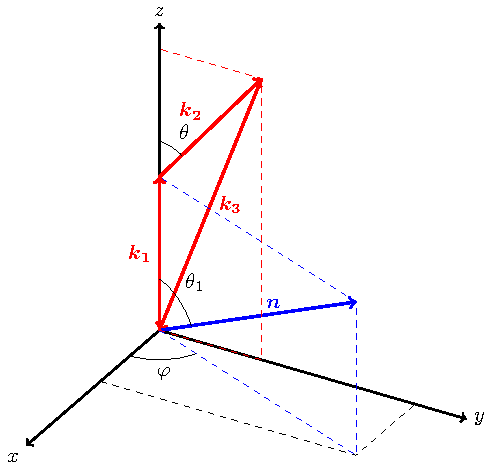
\includegraphics[width=0.6\linewidth]{fig/fig.pdf}
    \caption{Overview of the relevant vectors and angles for the Fourier-space bispectrum. \label{fig:geometry_overview1} }
\end{figure}       
Then we have $Y_{\ell m}(\mu_1,\varphi)$, so that we can write $B_g =\sum_{\ell m} B_{\ell m}Y_{\ell m}(\mu_1,\varphi)$. The leading relativistic terms we consider here generate odd-power multipoles up to $\ell=7$, and the full expression generates even and odd multipoles up to $\ell=8$-- see Chapter~\ref{chapter:multipoles}. 
Different powers of $(\i\mu_1)$ and $(\i\mu_2)$ contribute to the dipole as follows, \todo{check this table}
\begin{align}
\arraycolsep=1.0pt\def\arraystretch{1}
\int\mathrm{d}\Omega (\i\mu_1)^a  (\i \mu_2)^b Y^*_{1 m} & = 
 \delta_{m,0}\frac{\i\sqrt{3\pi}}{15}\left[ \begin {array}{ccccc} 
 0&10\mu&0&-6\mu  &\\ 
10&0&-4{\mu}^{2}-2&0& \cdots\\ 
0&-6\,\mu&0&{\frac {12{
\mu}^{3}+18\mu}{7}}& \\ 
-6&0&{\frac {24
\,{\mu}^{2}+6}{7}}&0& \\
 &\vdots & & & \ddots
\end {array} \right] \nonumber \\
& +
\delta_{m,\pm1}\frac{\sqrt{6\pi}}{15}
 \left[ \begin {array}{ccccc} 0&-5&0&3&\\ 
 0&0&2\,\mu&0
& \cdots\\ 
0&1&0&-\frac{6{\mu}^{2}+3}{7}&\\ 
0&0
&-\frac{6}{7}\,\mu&0&\\
 &\vdots & & & \ddots
\end {array} \right] \sin\theta\,,
\label{dkjsncdjcnsk}
\end{align}
where each matrix element corresponds to a particular combination of $a,b$,
where the matrix indices run over the values $a=0\ldots6, b=0\ldots6$, with powers above 3 not written above; these are polynomials in $\mu$ up to order 6. From this we can read off the terms from $\mathcal{K}_\text{D}$ contribute to differing $m=0,\pm1$. In particular, if $i+j$ is even~-- i.e., the real part of the bispectrum~--  there is no contribution: only the imaginary terms, corresponding to $i+j$ odd, contribute. For the monopole, only $i+j$ even contribute. Therefore, at $\ord(\cH/k)$, \emph{the monopole of the bispectrum is the Newtonian part, while the dipole is purely from the relativistic corrections.  The presence of the dipole is therefore a `smoking gun' signal for the leading relativistic correction to the bispectrum.} At order $\ord((\cH/k)^{2})$, relativistic terms appear in the monopole, which were considered in \citet{Umeh:2016nuh,Jolicoeur:2017nyt,Jolicoeur:2017eyi,Jolicoeur:2018blf}.\\


\section{Squeezed, equilateral and flattened limits}

It is relatively straightforward to understand the type of dipole generated in different triangular configurations in our conventions. In particular, for the $\ord(\cH/k)$ relativistic dipole:
\begin{itemize}
\item The squeezed case is zero for $m=0$, and is non-zero for $m=\pm1$. We see this directly from \eqref{dkjsncdjcnsk}: with $\mu=-1$ the $m=0$ contribution is anti-symmetric in $i,j$ while $\mathcal{B}_{ij}$ is symmetric in this limit.
\item In the equilateral case, the dipole is zero (this is the case for all orders in $\cH/k$).
\item The flattened case ($k_1=k_2=k_3/2,\theta=0$) is zero for $m=\pm1$ (for all orders in $\cH/k$), but is non-zero for $m=0$. This can be seen directly from \eqref{dkjsncdjcnsk} with $\theta=0$.
\end{itemize}
%Geometrically, we can understand these by rotating the triangle about its centre with respect to $\bm n$. For the equilateral case, the symmetry of the triangle means that the dipole part cancels out. For the flattened case, where there is a vertex at the centre, an anti-symmetry occurs only parallel to $\bm n$, and cancels in the plane orthogonal. For the squeezed case, this is anti-symmetric both along and perpendicular to $\bm n$, so excites both $m=\pm1$. 
 
To show the equilateral case is zero is a lengthy calculation involving many cancellations.  Let us illustrate instead the squeezed case. We write $k_1=k_2=\sqrt{1+\varepsilon^2}k_S, k_3=2\ep k_S$.
In this case the triangle has small angle $2\ep$ and equal angles $\pi/2-\ep$, where the squeezed limit is $\ep\to0$. It is convenient to replace $(1,2,3)$ by $(S,-S,L)$.
Then to $O(\ep)$,
$%\bea
k_{-S}= k_{S}\,,~~k_L=2\ep k_S\,,~~  
\mu_{-S}=-\mu_S-2\ep\mu_L\,,
%\nonumber\\&&
\mu_L = -\sqrt{1-\mu_S^2}\,\cos\varphi - {\ep\mu_S}\,.
%\hat{\k}_2=-\hat{\k}_1-2\ep\,\hat{\k}_3 \\ &&
$% \label{mu}
%\eea
 ~In this limit, the permutations of the relativistic kernels become
\begin{align}
% {\cal K}^{(2)}_{\mathrm{D}}(\k_S,\k_{-S},\k_L) &=&0\\
& {\cal K}^{(2)}_{\mathrm{D}}(\k_L,\k_S,\k_{-S}) = \i {\cH}
{\bigg[- \frac{3}{2}\Omega_m b_1\mu_S \frac{k_S}{k_L^2}+ C f \frac{\mu_L}{k_L} }
\nonumber\\
& - \frac{3}{2} \Omega_m f\mu_S^3 \frac{k_S}{k_L^2} +\Big( \frac{3}{2} \Omega_m- Ef \Big) f\mu_S^2 \frac{\mu_L}{k_L}\bigg] 
\label{k2d1} 
% {\cal K}^{(2)}_{\mathrm{D}}(\k_{-S},\k_L,\k_S) &=&  {\cal K}^{(2)}_{\mathrm{D}}(\k_L,\k_S,\k_{-S})\Big|_{\mu_S\to \roy{\mu_{-S}}}  \label{k2d2}
\end{align}
and $ {\cal K}^{(2)}_{\mathrm{D}}(\k_{-S},\k_L,\k_S) =  {\cal K}^{(2)}_{\mathrm{D}}(\k_L,\k_S,\k_{-S})\big|_{\mu_S\to {\mu_{-S}}}$ while ${\cal K}^{(2)}_{\mathrm{D}}(\k_S,\k_{-S},\k_L) =0$. 
In the squeezed limit of the cyclic sum~\eqref{eq:fsbispdef}, the terms $ {\cal K}^{(2)}(\k_L,\k_S,\k_{-S})$ and  ${\cal K}^{(2)}(\k_{-S},\k_L,\k_S)$ appear only in the form ${\cal K}^{(2)}(\k_L,\k_S,\k_{-S})+{\cal K}^{(2)}(\k_{-S},\k_L,\k_S)$. This sum regularises
the divergent $k_S/k_L=(2\ep)^{-1}$ and $k_S/k_L^2=(2\ep k_L)^{-1}$ terms.  We obtain the bispectrum in the squeezed limit,


\begin{align}
&B_{g}^{\mathrm{sq}} = b_{1S}b_{1L}b_{SL}\, P_LP_S+\i b_{1S}\Big\{b_{SL}f A + {\frac{3}{2}} \Omega_m b_{1S}b_{1L} 
\nonumber\\
&+2b_{1L}f C+ b_{1L}\mu_S^2\Big[{\frac{3}{2}}\Omega_m- Ef \Big] \Big\}P_LP_S\,\mu_L \frac{\cH}{k_L} \,,\label{bgd}
\end{align}


where $P_{S,L}=P(k_{S,L})$, $b_{1S,L}\equiv  b_1+f\mu_{S,L}^2$ and
\begin{align}
% \,, \label{b1sl}~~
b_{SL} \equiv 2b_2+ \frac{43}{21}b_1 - \frac{4}{21}
%\nonumber\\&&
+\Big(2b_1+ \frac{5}{7}\Big)f\mu_S^2%+b_1f\mu_L^2+{f^2}\mu_S^2\mu_L^2 
+f\mu_L^2 b_{1S}
\,. \nonumber\label{bsl}
\end{align}
%Note that we can neglect the $P(k_S)^2$ term relative to the $P(k_L)P(k_S)$ term in $B_{g {\mathrm{N}}}^{\rm sq}$.
Note that only the first term in the squeezed bispectrum comes from the Newtonian limit. 

The type of dipole extracted from this term is seen as follows. To this order we can write $\mu_{S}^2=\mu_{S}\mu_{-S}$. Then,  since $\mu_L=-2(\mu_S+\mu_{-S})/
\varepsilon$, we see that the $m=0$ term is zero because $B_{g {\mathrm{D}}}^{\mathrm{sq}}$ is symmetric in $\mu_{S}^i\mu_{-S}^j$ under $i\leftrightarrow j$, while the $m=0$ term is antisymmetric in~\eqref{dkjsncdjcnsk}. This leaves just the $m=\pm1$ contribution in \eqref{dkjsncdjcnsk}.




\begin{figure}%[htbp]
\begin{center}
%\includegraphics[width=\columnwidth]{flattened-squeezed-02}
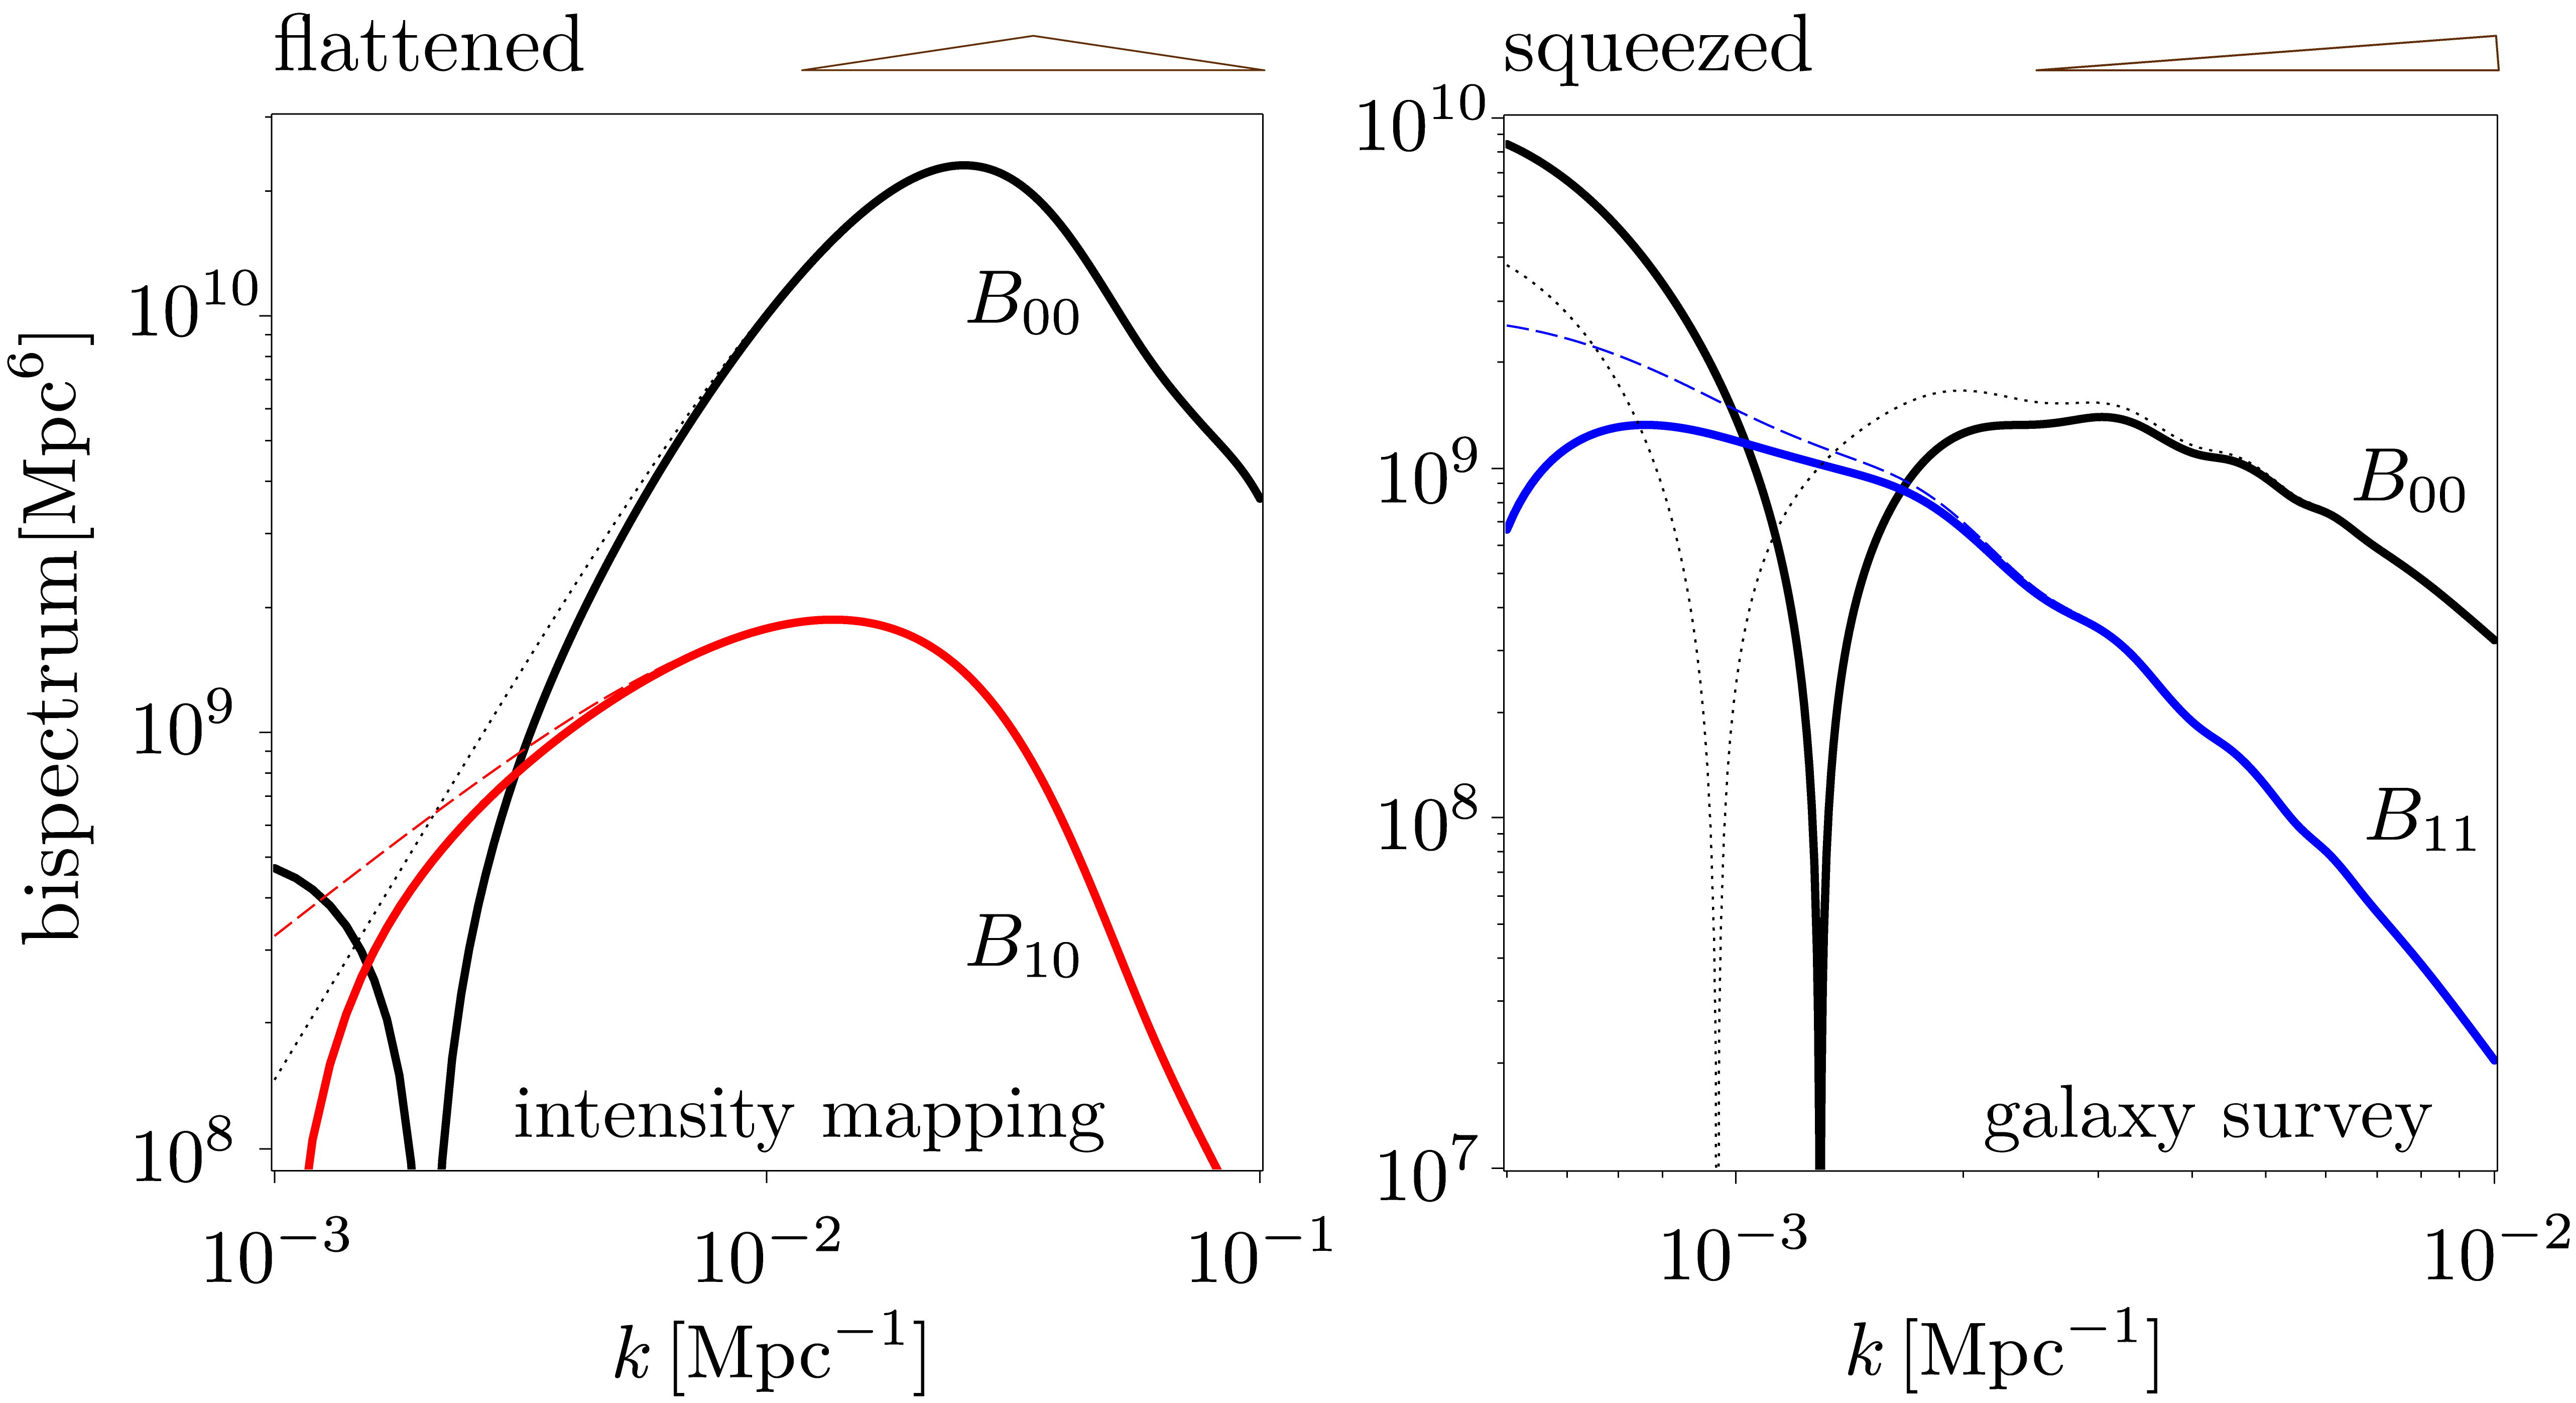
\includegraphics[width=\columnwidth]{fig/figuresv2-02}
\caption{ The absolute value of the bispectrum dipole at $z=1$  as a function of triangle size, in the flattened (Left, $\theta=2^\circ$, for intensity mapping bias) and squeezed (Right, $\theta=178^\circ$, for Euclid-like bias) configurations, with $k_3$ as the horizontal axis. Red is the $m=0$ part and blue is $m=\pm1$. Dashed (and dotted) lines show up to the $\ord(\cH/k)$ terms considered analytically here, while solid lines indicate larger-scale contributions. For reference the monopole is in black, with the dotted line the Newtonian part.  (The zero-crossing in the monopole for the squeezed case is a result of the tidal bias.)}
\label{snakcjnsdlkcans}
\end{center}
\end{figure}

\begin{figure}%[htbp]
\begin{center}
%\includegraphics[width=\columnwidth]{shapes-01}
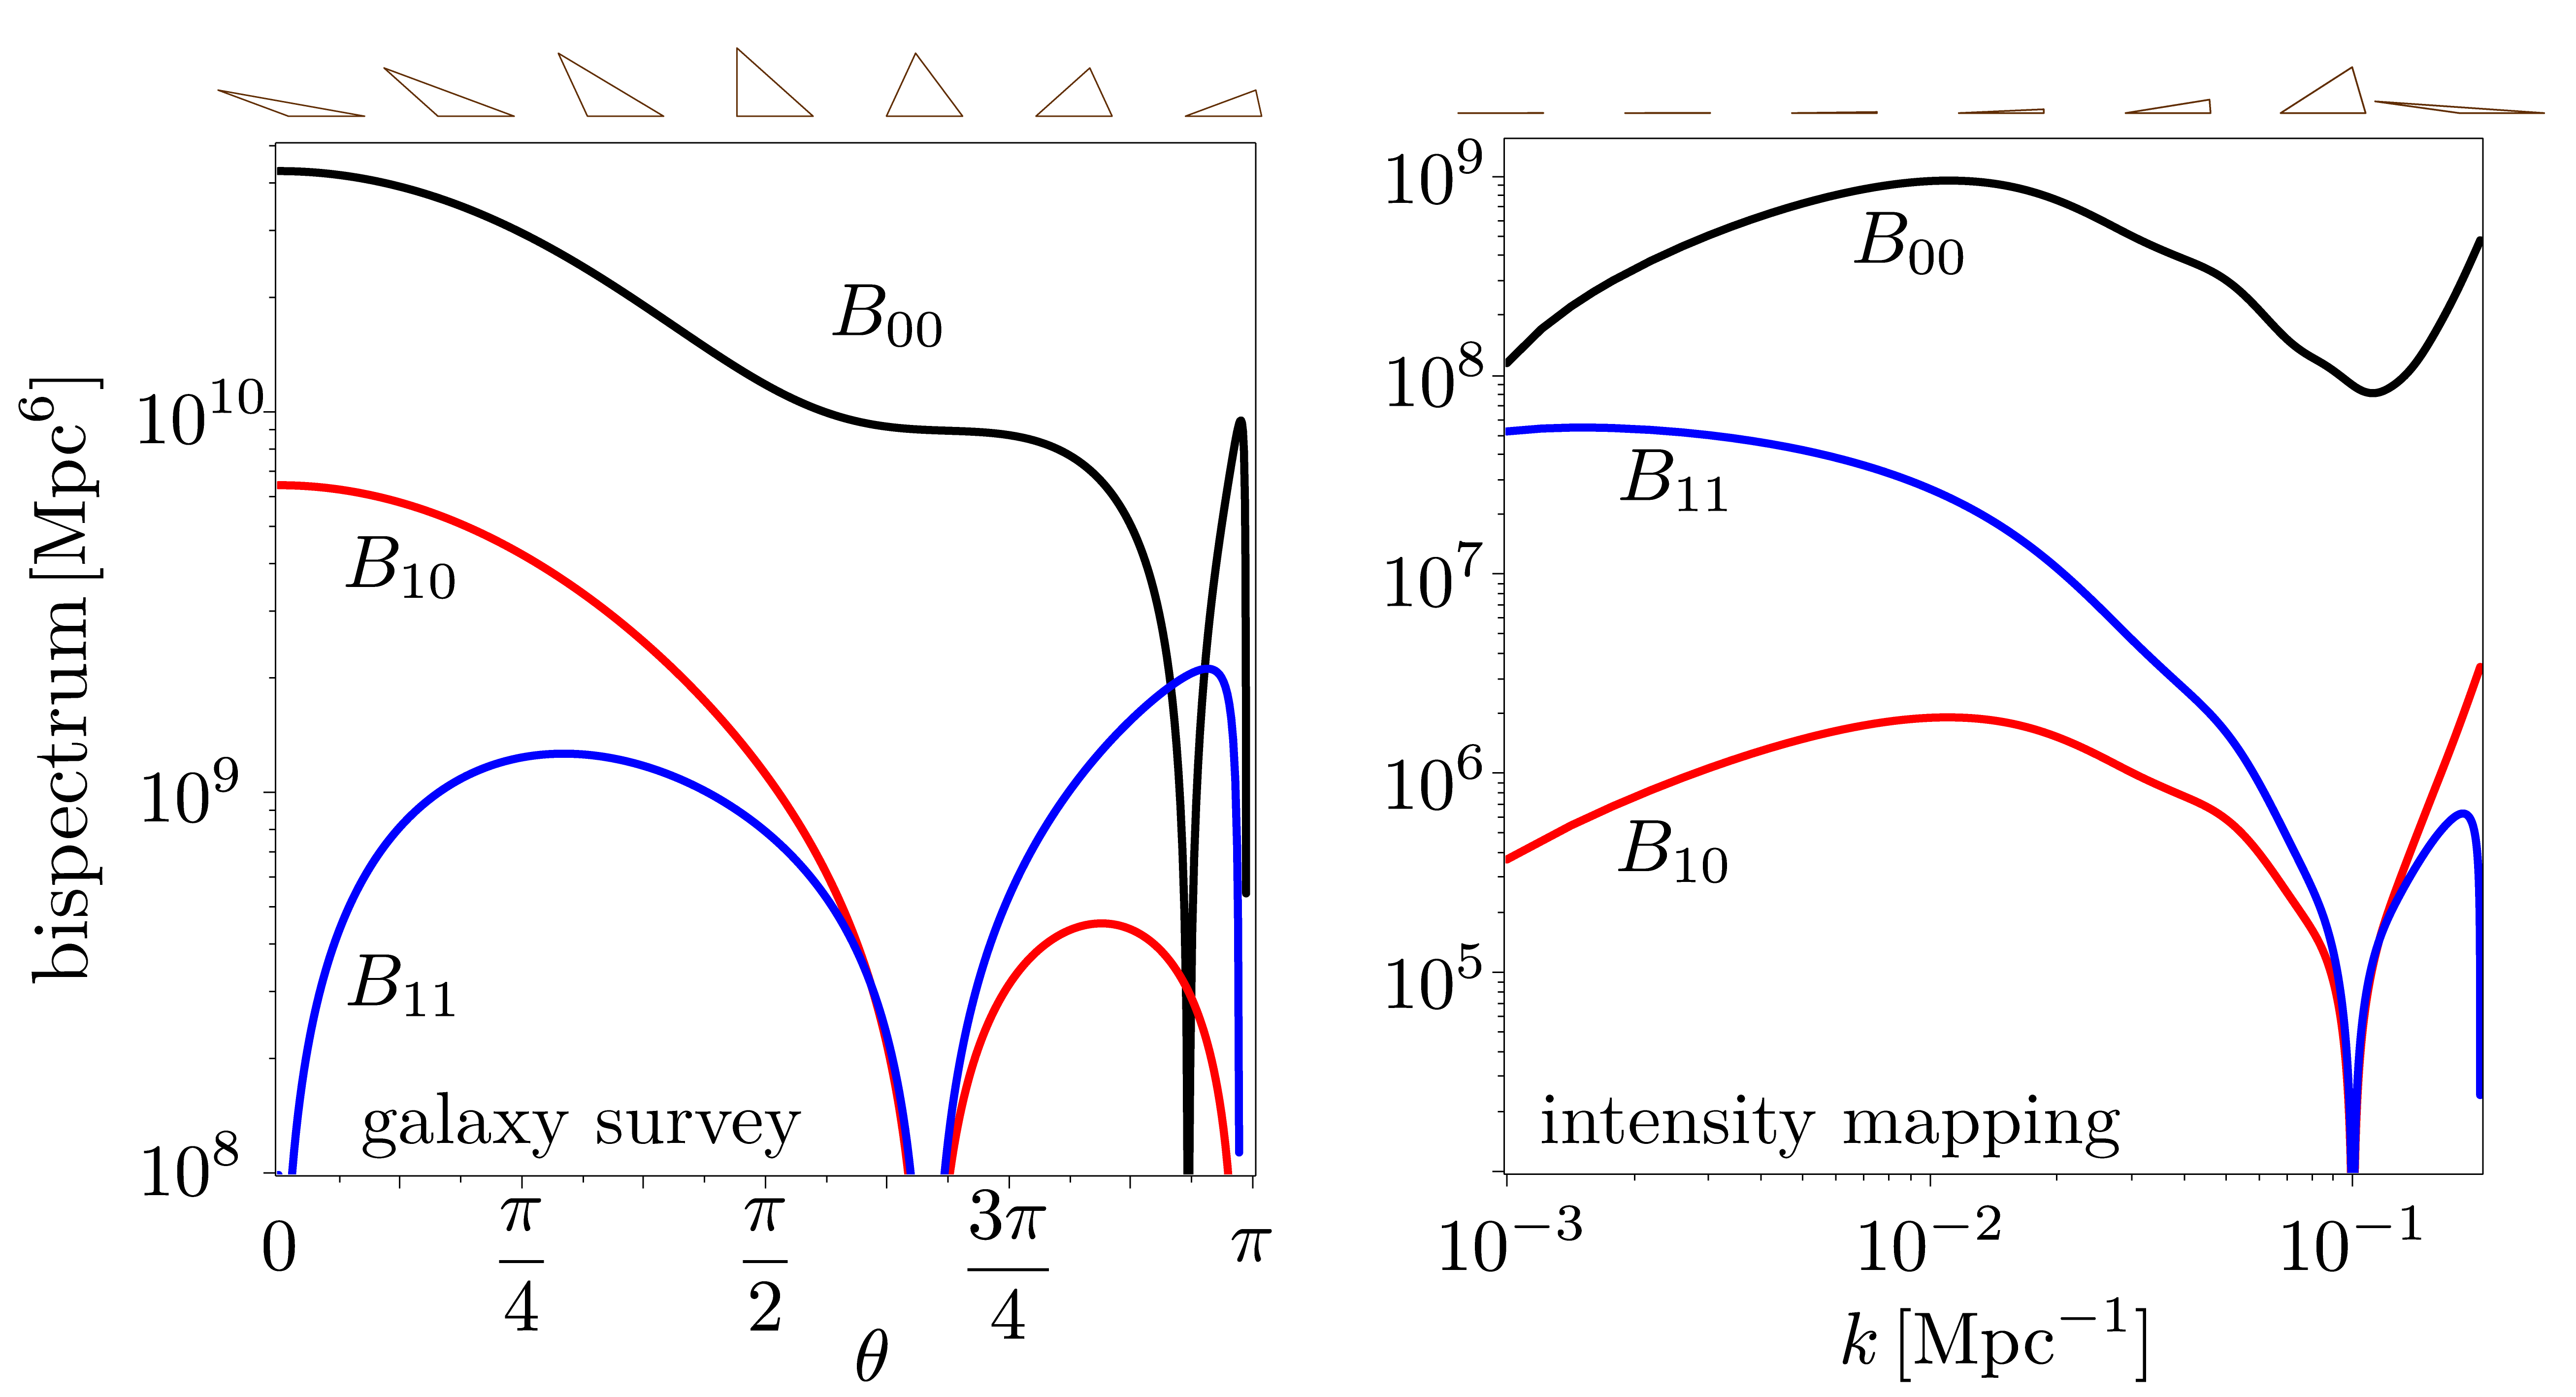
\includegraphics[width=\columnwidth]{fig/figuresv2-01}
\caption{ (Left) We show the dipoles as a function of $\theta$ with a bias appropriate for a Euclid-like survey, for $k_1=k_2=0.01$\,Mpc$^{-1}$. The left of the plot corresponds to the flattened case where the $m=0$ (red) dipole reaches 10\% of the monopole.  (Right) We show the IM signal with $k_1=k_2=0.1$\,Mpc$^{-1}$ versus the long mode $k_3$. Except for very long modes $\theta\approx\pi$, our $\ord(\cH/k)$ truncation is a very good approximation in these examples. }
\label{sankcjnakjdcs}
\end{center}
\end{figure}
 


\section{The dipole in intensity mapping and galaxy surveys}

We now consider the amplitude of the dipole relevant for upcoming galaxy surveys, which have different bias parameters. We consider two different types of survey: an SKA intensity mapping of 21\,cm radio emission, as well as a Euclid-like optical/infrared spectroscopic survey.
An intensity map of the 21cm emission of neutral hydrogen (HI) in the post-reionization Universe records the total emission in galaxies containing HI, without detecting individual galaxies. There is an equivalence between the brightness temperature contrast and number count contrast~\citep{Umeh:2015gza}. \todo{check the bias params, and provide expressions} For IM we use the bias parameters at $z=1$, 
$b_1 = 0.856, b_2 = -0.321, b_1' = -0.5\times10^{-4}, b_e = -0.5, b_e'=0, s = 2/5$~\citep{Fonseca:2018hsu,Umeh:2015gza}
while for the spectroscopic survey we use 
$ b_1 = 1.3,b_2 = -0.74, b_1' = -1.6\times10^{-4},  b_e = -4, b_e' = 0, s = -0.95$~\citep{Camera:2018jys,Yankelevich:2018uaz}.
For intensity mapping, $ \partial b_1/\partial \ln L =0$ and we assume it is zero for simplicity for the spectroscopic survey. We use a LCDM model with standard parameters $\Omega_m=0.314, h=0.67, f_\text{baryon}=0.157, n_s=0.968$. Plots are presented using linear power spectra generated using CAMB~\citep{Lewis:1999bs}.

In Fig.~\eqref{snakcjnsdlkcans} \todo{move figures into section} we show how changing the scale of a fixed triangle changes the amplitude of the dipole, with reference to the monopole. In the flattened case with $m=0$ we see the signal peaks for triangles below the equality scale, while for squeezed shapes, with $m=\pm1$, the signal is smaller, and peaks when the long mode approaches the Hubble scale. 
In Fig.~\eqref{sankcjnakjdcs} we change the shape with fixed $k_1=k_2$ for both galaxy and IM surveys. We confirm our analytical results that the equilateral limit is zero, as well as the other limits. For triangles between right-angle and flattened the dipole is more than 10\% of the monopole, and the signal is largest in the flattened case~-- except in the extreme squeezed limit (not shown). 


\section{Conclusions}

We have shown for the first time that the relativistic galaxy bispectrum has a leading correction which is a local dipole with respect to the observers line of sight. In contrast to the power spectrum, this dipole exists even for a single tracer. We have shown analytically how the dipole is generated for the leading terms, and numerically we have included all local contributions, which show up above the equality scale. We have neglected integrated terms which will also contribute to the dipole, but their inclusion in a Fourier space bispectrum is non-trivial. Local relativistic corrections will induce all multipoles up to $\ell=8$ at every $m$, in contrast to the Newtonian case which only induces even $\ell=0,2,4$. We will investigate these new multipoles in a forthcoming publication. 

We have shown that this dipole is large with respect to the monopole in both the flattened and squeezed limits, which excite different orders of the dipole orientation $m$.  We have shown that even on equality scales it is about 10\% of the monopole at $z=1$ for flattened shapes which have the largest amplitude. In more squeezed cases where the short mode is $\sim10$\,Mpc the dipole can also be a large part of the IM signal. Furthermore, although we have only considered Gaussian initial conditions here, the dipole will be unaffected by non-Gaussianity at leading order because these corrections start at $\ord((\cH/k)^2)$, making our predictions relatively robust to this. This implies that the dipole of the bispectrum is a unique signature of general relativity on cosmological scales, and therefore offers a new observational window onto modifications of general relativity. 





\chapter{Discussion and Outlook}
\label{chapter:disc}

In this thesis, we have investigated, starting in chapter \ref{chapter:intro}, ...
\begin{appendices}
%
\chapter{Beta coefficients}
\label{app_betas}
%
\begin{align} 
\frac{\beta_{1}}{\mathcal{H}^{4}} &= \frac{9}{4}\Omega_{m}^{2}\Bigg[6-2f\bigg(2b_{e}-4\Q-\frac{4(1-\Q)}{\chi\cH}-\frac{2\cH'}{\cH^{2}}\bigg)-\frac{2f'}{\cH}+b_{e}^{2}+5b_{e}-8b_{e}\Q + 4\Q + 16\Q^{2} \nonumber\\ 
& - 16\frac{\p \Q}{\p \ln{\bar{L}}} - 8\frac{\Q'}{\cH} + \frac{b_{e}'}{\cH}+\frac{2}{\chi^{2}\cH^{2}}\bigg(1-\Q+2\Q^{2}-2\frac{\p \Q}{\p \ln{\bar{L}}}\bigg)
 \nonumber\\ 
& - \frac{2}{\chi\cH}\bigg(3+2b_{e}-2b_{e}\Q-3\Q +8\Q^{2}-\frac{3\cH'}{\cH^{2}}(1-\Q) -8\frac{\p \Q}{\p \ln{\bar{L}}} - 2\frac{\Q'}{\cH}\bigg) \nonumber \\
& + \frac{\cH'}{\cH^{2}}\bigg(-7-2b_{e}+8\Q+\frac{3\cH'}{\cH^{2}}\bigg) - \frac{\cH''}{\cH^{3}}\Bigg] \nonumber \\
&  +\frac{3}{2}\Omega_{m}f\Bigg[5-2f(4-b_{e})+\frac{2f'}{\cH}+2b_{e}\bigg(5+\frac{2(1-\Q)}{\chi\cH}\bigg)-\frac{2b_{e}'}{\cH} -2b_{e}^{2} + 8b_{e}\Q - 28\Q \nonumber \\
& - \frac{14(1-\Q)}{\chi\cH}-\frac{3\cH'}{\cH^{2}} +4\bigg(2-\frac{1}{\chi\cH}\bigg)\frac{\Q'}{\cH}\Bigg] \nonumber \\
&  +\frac{3}{2}\Omega_{m}f^{2}\bigg[-2+2f-b_{e}+4\Q+\frac{2(1-\Q)}{\chi\cH}+\frac{3\cH'}{\cH^{2}}\bigg] \nonumber \\
&  +f^{2}\bigg[12-7b_{e}+b_{e}^{2}+\frac{b_{e}'}{\cH}+(b_{e}-3)\frac{\cH'}{\cH^{2}}\bigg] - \frac{3}{2}\Omega_{m}\frac{f'}{\cH} \\
\nonumber\\
%----------------
\frac{\beta_{2}}{\cH^{4}} &= \frac{9}{2}\Omega_{m}^{2}\bigg[-1+b_{e}-2\Q-\frac{2(1-\Q)}{\chi\cH}-\frac{\cH'}{\cH^{2}}\bigg] + 3\Omega_{m}f\bigg[-1+2f{-b_{e}}+4\Q+\frac{2(1-\Q)}{\chi\cH}+\frac{3\cH'}{\cH^{2}}\bigg] \nonumber \\
&  +3\Omega_{m}f^{2}\bigg[-1+b_{e}-2\Q-\frac{2(1-\Q)}{\chi\cH}-\frac{\cH'}{\cH^{2}}\bigg] + 3\Omega_{m}\frac{f'}{\cH}\; \\ 
%----------------
\frac{\beta_{3}}{\mathcal{H}^{3}} &= \frac{9}{4}\Omega_{m}^{2}(f-2+2\Q) \nonumber \\
&  + \frac{3}{2}\Omega_{m}f\Bigg[-2 -f\bigg(-3+f+2b_{e}-3\Q-\frac{4(1-\Q)}{\chi\cH}-\frac{2\cH'}{\cH^{2}}\bigg)-\frac{f'}{\cH}\nonumber \\
& +{3}b_{e}+b_{e}^{2}-6b_{e}\Q{+4}\Q +8\Q^{2}-8\frac{\p \Q}{\p \ln{\bar{L}}} -6\frac{\Q'}{\cH} +\frac{b_{e}'}{\cH} \nonumber \\
& +\frac{2}{\chi^{2}\cH^{2}}\bigg(1-\Q+2\Q^{2}-2\frac{\p \Q}{\p \ln{\bar{L}}}\bigg) + \frac{2}{\chi \cH}\bigg({-1} -2b_{e}+2b_{e}\Q{+}\Q-6\Q^{2}  \nonumber \\
& +\frac{3\cH'}{\cH^{2}}(1-\Q) +6\frac{\p \Q}{\p \ln{\bar{L}}} + 2\frac{\Q'}{\cH}\bigg) -\frac{\cH'}{\cH^{2}}\bigg({3}+2b_{e}-6\Q-\frac{3\cH'}{\cH^{2}}\bigg) - \frac{\cH''}{\cH^{3}}\Bigg] \nonumber \\
&  {+} f^{2}\Bigg[-3+2b_{e}\bigg(2+\frac{(1-\Q)}{\chi\cH}\bigg)-b_{e}^{2}+2b_{e}\Q -6\Q-\frac{b_{e}'}{\cH}-\frac{6(1-\Q)}{\chi\cH}\nonumber \\
& +2\bigg(1-\frac{1}{\chi\cH}\bigg)\frac{\Q'}{\cH}\Bigg]  \\ 
%----------------
\frac{\beta_{4}}{\cH^{3}} &= \frac{9}{2}\Omega_{m}f\bigg[-b_{e}+2\Q+\frac{2(1-\Q)}{\chi \cH}+\frac{\cH'}{\cH^{2}}\bigg]\\ 
%----------------
{{\frac{\beta_5}{\cH^{3}}}} &= 3\Omega_{m}f\bigg[b_{e}-2\Q-\frac{2(1-\Q)}{\chi\cH}-\frac{\cH'}{\cH^{2}}\bigg] \\ 
%------
\frac{\beta_6}{\cH^{2}} &= \frac{3}{2}\Omega_{m}\Bigg[2-2f+b_{e}-4\Q-\frac{2(1-\Q)}{\chi\cH}-\frac{\cH'}{\cH^{2}}\Bigg] \\
%---------
\frac{\beta_7}{\cH^{2}} &= f(3-b_{e}) \\ 
%----------------
\frac{\beta_8}{\cH^{2}} &= {3\Omega_{m}f(2-f-2\Q)} + f^{2}\Bigg[4+b_{e}-b_{e}^{2}+4b_{e}\Q-{6}\Q-4\Q^{2}+4\frac{\p \Q}{\p \ln{\bar{L}}} + 4\frac{\Q'}{\cH} - \frac{b_{e}'}{\cH}  \nonumber \\\nonumber\\
& - \frac{2}{\chi^{2}\cH^{2}}\bigg(1-\Q+2\Q^{2}-2\frac{\p \Q}{\p \ln{\bar{L}}}\bigg) - \frac{2}{\chi\cH}\bigg(3-2b_{e}+2b_{e}\Q-\Q-4\Q^{2}+\frac{3\cH'}{\cH^{2}}(1-\Q) \nonumber\\
& + 4\frac{\p \Q}{\p \ln{\bar{L}}} + 2\frac{\Q'}{\cH}\bigg) - \frac{\cH'}{\cH^{2}}\bigg(3-2b_{e}+{4}\Q+\frac{3\cH'}{\cH^{2}}\bigg) + \frac{\cH''}{\cH^{3}}\Bigg] \\ 
%----------------
\frac{\beta_{9}}{\cH^{2}} &= -\frac{9}{2}\Omega_{m}f \\ 
%----------------
{\frac{\beta_{10}}{\cH^{2}}} &= 3\Omega_{m}f \\ 
%----------------
\frac{\beta_{11}}{\cH^{2}} &= 3\Omega_{m}\bigg(\frac{1}{2}+f\bigg) + f - f^{2}\Bigg[-1+b_{e}-2\Q- \frac{2(1+\Q)}{\chi\cH}-\frac{\cH'}{\cH^{2}}\Bigg] \\ 
%-----------------
\frac{\beta_{12}}{\cH^{2}} &= \frac{3}{2}\Omega_{m}\Bigg[-2+b_{1}\bigg(2+b_{e}-4\Q-\frac{2(1-\Q)}{\chi\cH} -\frac{\cH'}{\cH^{2}}\bigg) + \frac{b_{1}'}{\cH} + 2\bigg(2-\frac{1}{\chi\cH}\bigg)\frac{\p b_{1}}{\p \ln{\bar{L}}}\Bigg] \nonumber \\
&- f\Bigg[2+b_{1}(f-3+b_{e}) + \frac{b_{1}'}{\cH}\Bigg]  \\ 
%----------------
\frac{\beta_{13}}{\cH^{2}} &= \frac{9}{4}\Omega_{m}^{2} {+ \frac{3}{2}\Omega_{m}f\Bigg[1-2f+2b_{e}-{6}\Q-\frac{4(1-\Q)}{\chi\cH}-\frac{3\cH'}{\cH^{2}}\Bigg]} + f^{2}(3-b_{e}) \\ 
%----------------
\frac{\beta_{14}}{\cH} &= -\frac{3}{2}\Omega_{m}b_{1} \\
%----------------
\frac{\beta_{15}}{\cH} &= 2f^{2}  \\ 
%----------------
\frac{\beta_{16}}{\cH} &= f\Bigg[b_{1}\bigg(f+b_{e}-2\Q-\frac{2(1-\Q)}{\chi\cH}-\frac{\cH'}{\cH^{2}}\bigg) + \frac{b_{1}'}{\cH} + 2\bigg(1-\frac{1}{\chi\cH}\bigg)\frac{\p b_{1}}{\p \ln \bar{L}}\Bigg] \\
%----------------
\frac{\beta_{17}}{\cH} &= -\frac{3}{2}\Omega_{m}f \\
%----------------
\frac{\beta_{18}}{\cH} &= \frac{3}{2}\Omega_{m}f -f^{2}\Bigg[3-2b_{e}+{4}\Q+\frac{4(1-\Q)}{\chi\cH}+\frac{3\cH'}{\cH^{2}}\Bigg] \\
%----------------
\frac{\beta_{19}}{\cH} &= f\Bigg[b_{e}-2Q-\frac{2(1-\Q)}{\chi\cH}-\frac{\cH'}{\cH^{2}}\Bigg] 
\end{align}
%
\chapter{Beta coefficient tables}
\label{app_pnga}
%
% \begin{longtable}{| p{.20\textwidth} | p{.80\textwidth} |} 
% \caption{Your caption here}\\
% \hline
% foo & bar \\ \hline 
% foo & bar \\ \hline
% foo & bar \\ \hline
% foo & bar \\ \hline
% foo & bar \\ \hline
% foo & bar \\ \hline
% foo & bar \\ \hline
% foo & bar \\ \hline
% foo & bar \\ \hline
% foo & bar \\ \hline
% foo & bar \\ \hline
%  % needs to go inside longtable environment
% \label{tabc1}
% \end{longtable}

Here we present a table of individual terms in the observed density fluctuation $\Delta_g^{(2)}$, with the corresponding $\beta$ function $\beta_I$ in the second column (N for standard Newtonian terms), Fourier space kernel $\mathcal{F}$, and the coefficients of the terms that appear in $\Delta_g^{(2)}$ in the fourth column. 

\begingroup
\tiny
\begin{longtable}{| c | c | c | c |} 
\caption{ {Individual terms in the observed $\Delta_g^{(2)}(a,\bm{x})$ [see \eqref{eq:SecondorderNewtonian}, \eqref{odg2}] for $\fnl=0$ are shown in column 1. The related $\beta_I$ functions in \eqref{e2.23} are listed in column 2. The Fourier-space kernels ${\cal F}$  corresponding to column 1, given by 
$ \int \!{\ud \k'}\, {\cal F}(\k',\k-\k')\delta_{\mathrm{T}}(\k')\delta_{\mathrm{T}}(\k-\k')/(2\pi)^3$, are shown in column~3. Column 4 gives
the coefficients of the terms in $\Delta_g^{(2)}$ (column 1). The line-of-sight derivative is $\partial_\|=\bm{n}\!\cdot\!\bm{\nabla}$ and $\Phi=\Psi$.
The superscript (1) on first-order quantities has been omitted and N denotes Newtonian. This table updates the one in \cite{Jolicoeur:2017nyt}.}} \label{tabc1} \\
\hline 
&  &  & \\
TERM & $~~\beta~~$ & FOURIER KERNEL    & COEFFICIENT \\ 
&  &  & \\ \hline \hline
&  &  & \\
%%----------------------- Newtonian
$\delta^{(2)}_{\mathrm{T,{N}}}$ & N & $F_{2}(\!\bm{k}_{1},\!\bm{k}_{2}\!)$ & $b_{10}$ \\ 
&  &  & \\
%%-----------------------
${\big(\delta_{\mathrm{T}}\big)^2}$ & N & 1 & $b_{20}$ \\ 
&  &  & \\
%%-----------------------
${s^2}$ & N & $S_2(\!\bm{k}_{1},\!\bm{k}_{2}\!)$ & $b_{s}$ \\ 
&  &  & \\
%%-----------------------
$\partial_{\parallel}^{2}V^{(2)}_{{\mathrm{N}}}$ & N & $f^{2}\cH \mu_{3}^{2}G_{2}(\!\bm{k}_{1},\!\bm{k}_{2}\!)$ & $-1/\cH$ \\ 
&  &  & \\
%%-----------------------
$\delta_{\mathrm{T}}\partial_{\parallel}^{2}V$ & N & $-f\cH \big(\mu_{1}^{2} + \mu_{2}^{2}\big)/2 $ & $-2b_{10}/\cH$ \\
&  &  & \\ 
%%-----------------------
$\partial_{\parallel}V \partial_{\parallel}\delta_{\mathrm{T}}$ & N\ & $-f\cH {{\mu_{1}\mu_{2}\big(k_{1}^{2} + k_{2}^{2}\big)}/{\big(2k_{1}k_{2}\big)}}$& $-2b_{10}/\cH$ \\ 
&  &  & \\
%%-----------------------
$\partial_{\parallel}V \partial_{\parallel}^{3}V $  & N & $f^{2} \cH^2{{\big(\mu_{1}\mu_{2}^{3}k_{2}^{2} + \mu_{2}\mu_{1}^{3}k_{1}^{2}\big)}/{\big(k_{1}k_{2}\big)}}$ & $ {2}/{\cH^{2}}$  \\
&  &  & \\ 
%%-----------------------
$\big[\partial_{\parallel}^{2}V\big]^{2}$  & N &$f^{2}\cH^2 \,\mu_{1}^{2}\mu_{2}^{2}$ & ${2}/{\cH^{2}}$ \\ 
&  &  & \\
\hline 
&  &  & \\
%%----------------------- beta_{1}, beta_{2}
$\big(\Psi\big)^{2}$ & $\beta_{1}$ & ${9}\Omega_{m}^{2}\cH^{4}/{\big(4k_{1}^{2}k_{2}^{2}\big)}$ & $\mathcal{A}_{1}$ \\ 
&  &  & \\
%%-----------------------
${\Psi V}$ & $\beta_{1}$ & $-{3}\Omega_{m}\cH^{3}f/{\big(2k_{1}^{2}k_{2}^{2}\big)}$  & $\mathcal{A}_{2}$ \\ 
&  &  & \\
%%-----------------------
$VV' $ & $\beta_{1}$  & ${ f\cH^{3}\big(3\Omega_{m}-2f\big)/{\big(2k_{1}^{2}k_{2}^{2}\big)} }$ & $ (b_{e}-3)\cH$ \\ 
&  &  & \\
%%-----------------------
$\big(V\big)^{2}$ & $\beta_{1}$ & $f^{2} \cH^{2}/{\big(k_{1}^{2}k_{2}^{2}\big)}$ & $(b_{e}-3)^{2}\cH^2+{b_{e}'\cH} +(b_{e}-3){\cH'} $ \\ 
&  &  & \\
%%-----------------------
${V^{(2)}_{\mathrm{GR}}}$ & $\beta_1,\beta_2$ & $-3\Omega_{m}\cH^{3}\big[3 -2 E_{2}(\!\bm{k}_{1},\!\bm{k}_{2},\!\bm{k}_{3}\!)\big]/\big(4k_{1}^{2}k_{2}^{2}\big)$ & $(3-b_{e})\cH$ \\
&  &  & \\
%%-----------------------
${\Phi^{(2)}_{\mathrm{GR}}}$ & $\beta_1,\beta_2$ & $3\Omega_{m}\cH^{4}\big[{f-\mathcal{C}_1 + \mathcal{C}_1} E_{2}(\!\bm{k}_{1},\!\bm{k}_{2},\!\bm{k}_{3}\!)\big]/\big(2k_{1}^{2}k_{2}^{2}\big)$ & $1-b_e+2\Q+\mathcal{R}$ \\
&  &  & \\
%%-----------------------
${\Psi^{(2)}_{\mathrm{GR}}}$ & $\beta_1,\beta_2$ & $3\Omega_{m}\cH^{4}\big[{\mathcal{C}_1-3f+2f^2 +2 f} E_{2}(\!\bm{k}_{1},\!\bm{k}_{2},\!\bm{k}_{3}\!)\big]/\big(2k_{1}^{2}k_{2}^{2}\big)$ & $2\big(\Q - 1\big)$ \\
&  &  & \\
%%-----------------------
${\Psi^{(2)\prime}_{\mathrm{GR}}}$ & $\beta_1,\beta_2$ & $3\Omega_{m}\cH^{5}\big[{\mathcal{C}_2 +  \mathcal{C}_{3}} E_{2}(\!\bm{k}_{1},\!\bm{k}_{2},\!\bm{k}_{3}\!)\big]/\big(2k_{1}^{2}k_{2}^{2}\big)$ & ${1}/{\cH}$ \\
%%-----------------------
&  &  & \\
\hline 
&  &  & \\
%%----------------------- beta_{3}
$V\partial_{\parallel}V $ & $\beta_{3}$ & $ \mathrm{i}\,f^{2}\cH^{2}
{\big(\mu_{1}k_{1} + \mu_{2}k_{2}\big)}/{\big(2k_{1}^{2}k_{2}^{2}\big)}$ &  $\mathcal{A}_{3}$ \\ 
&  &  & \\
%%-----------------------
$\Psi\partial_{\parallel}V$ & $\beta_{3}$ & $-{\i}\,3f\Omega_{m}\cH^{3}\,{\big(\mu_{1}k_{1} + \mu_{2}k_{2}\big)}/{\big(4k_{1}^{2}k_{2}^{2}\big)}$ & $\mathcal{A}_{4}$ \\ 
&  &  & \\
%%-----------------------
$\Psi\partial_{\parallel}\Phi$ & $\beta_{3}$ & ${\i}\,9\Omega_{m}^{2}\cH^{4}{\big(\mu_{1}k_{1} + \mu_{2}k_{2}\big)}/{\big(8k_{1}^{2}k_{2}^{2}\big)}$ & ${2}(f-2+2\mathcal{Q})/{\cH}$  \\ 
&  &  & \\
\hline
&  &  & \\ 
%%----------------------- beta_{4}, beta_{5}
${\partial_{\parallel}V^{(2)}_{\mathrm{GR}}}$ & $\beta_{4},\beta_{5}$ & $-\mathrm{i}\,3\Omega_{m}\cH^{3}\big[3 -2 E_{2}(\!\bm{k}_{1},\!\bm{k}_{2},\!\bm{k}_{3}\!)\big]\mu_3 k_3/\big(4k_{1}^{2}k_{2}^{2}\big)$ & $b_{e}-2Q-\mathcal{R}$ \\
&  &  & \\
\hline
&  &  & \\ 
%%----------------------- beta_{6}
${\Psi^{(2)}_{\mathrm{N}}=\Phi^{(2)}_{\mathrm{N}}}$ & $\beta_{6}$ & $-{3}\Omega_{m}{\cH^{2}}F_{2}(\!\bm{k}_{1},\!\bm{k}_{2}\!)/{\big(2k_{3}^{2}\big)}$ & $4\mathcal{Q}-1-b_{e}+\mathcal{R}$ \\
&  &  & \\ 
%%-----------------------
${\Psi_{\mathrm{N}}^{(2)\prime} = \Phi_{\mathrm{N}}^{(2)\prime}}$  & $\beta_{6}$ & $-{3}\Omega_{m}{\cH^{3}}(2f-1)F_{2}(\!\bm{k}_{1},\!\bm{k}_{2}\!)/{\big(2k_{3}^{2}\big)}$ & ${1}/{\cH}$ \\
&  &  & \\ 
\hline\
&  &  & \\ 
%%----------------------- beta_{7}
$V^{(2)}_{\mathrm{N}}$ & $\beta_{7}$ & $f{\cH}G_{2}(\!\bm{k}_{1},\!\bm{k}_{2}\!)/{k_{3}^{2}}$ & $(3-b_{e})\cH$ \\ 
&  &  & \\
\hline 
&  &  & \\
%%----------------------- beta_{8}
$\big(\partial_{\parallel}V\big)^{2} $ & $\beta_{8}$ & $-f^{2}\cH^{2}{\mu_{1}\mu_{2}}/{\big(k_{1}k_{2}\big)}$ & $\mathcal{A}_{5}$ \\
&  &  & \\ 
%%-----------------------
$\partial_{\parallel}V\partial_{\parallel}\Psi$ & $\beta_{8}$ & ${3}f\Omega_{m}\cH^{3}{\mu_{1}\mu_{2}/{\big(2k_{1}k_{2}\big)}}$ & ${2}(2-f-2\mathcal{Q})/{\cH}$ \\
&  &  & \\ 
\hline
&  &  & \\ 
%%----------------------- beta_{9}, beta_{10}
${\partial_{\parallel}^{2}V^{(2)}_{\mathrm{GR}}}$ & $\beta_{9},\beta_{10}$ & $\mathrm{i}\,3\Omega_{m}\cH^{3}\big[3 -2 E_{2}(\!\bm{k}_{1},\!\bm{k}_{2},\!\bm{k}_{3}\!)\big]\mu_3^{2} k_3^{2}/\big(4k_{1}^{2}k_{2}^{2}\big)$ & $-1/\cH$ \\
&  &  & \\ 
\hline
&  &  & \\ 
%%----------------------- beta_{11}
$\partial_{i}V\,\partial^{i}V$ & $\beta_{11}$ & $-f^{2}\cH^{2}\,{\bm{k}_1\!\cdot\! \bm{k}_2}/{\big(k_{1}^{2}k_{2}^{2}\big)}$  & $ b_{e} -1- 2\mathcal{Q} - \mathcal{R}$ \\ 
&  &  & \\
%%-----------------------
$\partial_{i}V\partial^{i}\Psi$  &$\beta_{11}$ & $3f\Omega_{m}\cH^{3} \,{\bm{k}_{1}\!\cdot\! \bm{k}_{2}}/{\big(2k_{1}^{2}k_{2}^{2}\big)} $ & ${2}/{\cH}$  \\
&  &  & \\ 
\hline 
&  &  & \\
%%----------------------- beta_{12}
${\Psi\delta_{\mathrm{T}}}$ & $\beta_{12}$ &$-{3}\Omega_{m}\cH^{2}{\big(k_{1}^{2}+k_{2}^{2}\big)}/{\big(4k_{1}^{2}k_{2}^{2}\big)} $& $2b_{10}\big(4\mathcal{Q}+\mathcal{R} -2-b_{e}\big) -{\mathcal{S}}$  \\ 
&  &  & \\
%%-----------------------
${V \delta_{\mathrm{T}}}$& $\beta_{12}$ & $f\cH{\big(k_{1}^{2}+k_{2}^{2}\big)}/{\big(2k_{1}^{2}k_{2}^{2}\big)} $  & $b_{10}' + 2b_{10}\big(3-b_e-f\big)\cH$ \\ 
&  &  & \\
\hline 
&  &  & \\
%%----------------------- delta2-gr
{$\delta^{(2)}_{{g \mathrm{T,GR}}}$}& ${\beta_{11},\beta_{12}}$ & {$\big(3\Omega_m+2f\big)\cH^2\big[\bm{k}_{1}\cdot\!\bm{k}_{2}-2\big(k_1^2+k_2^2\big)\big]/\big(2k_{1}k_{2}\big)$} & 1 \\
&  &  & \\ 
\hline
&  &  & \\
%%----------------------- beta_{13}
$\Psi \partial^{2}_{\parallel}V$ & $\beta_{13}$ & ${3}f\Omega_{m}\cH^{3}{\big(\mu_{1}^{2}k_{1}^{2} + \mu_{2}^{2}k_{2}^{2}\big)}/{\big(4k_{1}^{2}k_{2}^{2}\big)}$ &${2}\big[{1}-2f+2b_{e}-{6}\mathcal{Q}-2{\cal R}-\big({\cH'}/{\cH^{2}}\big)\big]/{\cH}$ \\ 
&  &  & \\
%%-----------------------
$\Psi\partial_{\parallel}^{2}\Psi $ & $\beta_{13}$ & $- {9}\Omega_{m}^2\cH^{4}{\big(\mu_{1}^{2}k_{1}^{2} + \mu_{2}^{2}k_{2}^{2}\big)}/{\big(4k_{1}^{2}k_{2}^{2}\big)}$ & $-{2}/{\cH^{2}}$  \\ 
&  &  & \\
%%-----------------------
$V\partial_{\parallel}^{2}V$ &$\beta_{13}$ & $-f^2\cH^{3}{\big(\mu_{1}^{2}k_{1}^{2} + \mu_{2}^{2}k_{2}^{2}\big)}/{\big(2k_{1}^{2}k_{2}^{2}\big)}$ & ${2}(b_{e}-3)/{\cH}$ \\ 
&  &  & \\
%%----------------------- beta_{14}
$\Psi\partial_{\parallel}\delta_{\mathrm{T}}$ &$\beta_{14}$ & $-{\i}\,3\Omega_{m}\cH^2 {\big(\mu_{1}k_{1}^{3} + \mu_{2}k_{2}^{3}\big)}/{\big(4k_{1}^{2}k_{2}^{2}\big)}$& ${2}b_{10}/{\cH}$ \\ 
&  &  & \\
\hline
&  &  & \\
%%----------------------- beta_{15}
$\partial_{i}V\partial_{\parallel}\partial^{i}V $ & $\beta_{15}$ &$ -\mathrm{i}\,f^2\cH^2 \bm{k}_{1}\!\cdot\! \bm{k}_{2}{\big(\mu_{1}k_{1} + \mu_{2}k_{2}\big)}/{\big(2k_{1}^{2}k_{2}^{2}\big)}$ & $-{4}/{\cH}$ \\ 
&  &  & \\
\hline 
&  &  & \\
%%----------------------- beta_{16}
${\delta_{\mathrm{T}}\partial_{\parallel}V}$ & $\beta_{16}$ & $\mathrm{i}\,f\cH{\big(\mu_{1}k_{2} + \mu_{2}k_{1}\big)}/{\big(2k_{1}k_{2}\big)}$ & $2b_{10}\big(f+b_e-2\Q-\mathcal{R}\big)+{\mathcal{S}}$  \\ 
&  &  & \\
\hline
&  &  & \\ 
%%----------------------- beta_{17}
$\Phi\partial_{\parallel}^{3}V$ & $\beta_{17}$ & ${\i}\,3f\Omega_{m}\cH^3 {\big(\mu_{1}^{3}k_{1}^{3} + \mu_{2}^{3}k_{2}^{3}\big)}/{\big(4k_{1}^{2}k_{2}^{2}\big)}$ & $-{2}/{\cH^{2}}$ \\ 
&  &  & \\
\hline 
&  &  & \\
%%----------------------- beta_{18}
$\partial_{\parallel}V\partial^{2}_{\parallel}V$ & $\beta_{18}$ & $-\mathrm{i}\,f^{2}\cH^2 {{\big(\mu_{1}\mu_{2}^{2}k_{2} +\mu_{2}\mu_{1}^{2}k_{1}\big) }/{\big(2k_{1}k_{2}\big)}}$ & ${2}\big[3-2b_{e}+{4}\mathcal{Q}+2{\cal R}+\big({\cH'}/{\cH^{2}}\big)\big]/{\cH}$ \\ 
&  &  & \\
%%-----------------------
$\partial_{\parallel}V\partial^{2}_{\parallel}\Psi$ & $\beta_{18}$ & ${\i}\,3f\Omega_{m}\cH^3{{\big(\mu_{1}\mu_{2}^{2}k_{2} +\mu_{2}\mu_{1}^{2}k_{1}\big) }/{\big(4k_{1}k_{2}\big)}}$ & ${2}/{\cH^{2}}$ \\ 
&  &  & \\
\hline 
&  &  & \\
%%----------------------- beta_{19}
$\partial_{\parallel}{V_{\mathrm{N}}^{(2)}}$& $\beta_{19}$ & $\mathrm{i}\,f\cH \,{\mu_{3}}G_{2}(\!\bm{k}_{1},\!\bm{k}_{2}\!)/{k_{3}}$ & $b_{e}-2Q-\mathcal{R}$ \\
&  &  & \\ 
\hline
\end{longtable}
\endgroup

\noindent Here the ${\cal C}$ functions in the Fourier kernels are
\begin{align}
{\mathcal{C}_{1}} &= 2f - f^2 -3\Omega_m\;, \label{e7} \\
%\mathcal{C}_{2} &=& \frac{1}{2}\big(3\Omega_m -2f +2f^{2}\big)\;, \label{e8}\\
%\mathcal{C}_{3} &=& \frac{1}{2}\big(3\Omega_m + f - f^{2}\big)\;, \label{e9}\\
\mathcal{C}_{2} &= 2f-1+ \big(1-f\big)\bigg[6\Omega_m + f\big(1-2f\big) - 2f\frac{\cH'}{\cH^{2}}\bigg] \;, \label{e10} \\
%\mathcal{C}_{5} &=& \frac{1}{2}\big(2f-1\big)\;, \label{e11} \\
\mathcal{C}_{3} &= 2 f\bigg(2f-1+\frac{\cH'}{\cH^{2}}\bigg) +2 \frac{f'}{\cH}\;, \label{e12} 
\end{align}
the 
${\cal A}$ functions in the coefficients are 
\begin{align}
\mathcal{A}_{1} &= {-3} +2f\bigg({2}-2b_{e}+{4}\mathcal{Q}+\frac{4(1-\mathcal{Q})}{\chi\cH} +\frac{2\cH'}{\cH^{2}}\bigg) -\frac{2f'}{\cH} +b_{e}^{2}+ 6b_{e}-8b_{e}\mathcal{Q}+4\mathcal{Q} \nonumber \\
& +16\mathcal{Q}^{2} -16\frac{\partial \mathcal{Q}}{\partial \ln{L}} -8\frac{\mathcal{Q}'}{\cH} + \frac{b_{e}'}{\cH}+\frac{2}{\chi^{2}\cH^{2}}\bigg(1-\mathcal{Q}+2\mathcal{Q}^{2}-2\frac{\partial \mathcal{Q}}{\partial \ln{{L}}}\bigg)  \nonumber\\ 
& - \frac{2}{\chi\cH}\bigg[4+2b_{e}-2b_{e}\mathcal{Q}-4\mathcal{Q}+8\mathcal{Q}^{2}-\frac{3\cH'}{\cH^{2}}(1-\mathcal{Q})- 8\frac{\partial \mathcal{Q}}{\partial \ln{{L}}} - 2\frac{\mathcal{Q}'}{\cH}\bigg] \nonumber \\
& + \frac{\cH'}{\cH^{2}}\bigg(-8-2b_{e}+{8}\mathcal{Q}+\frac{3\cH'}{\cH^{2}}\bigg) - \frac{\cH''}{\cH^{3}}\;, \label{e2} 
\end{align}
\begin{align}
\mathcal{A}_{2} &= 2\cH\bigg[-\frac{15}{2}+f(3-b_{e})-\frac{3}{2}b_{e}-2b_{e}\frac{(1-\mathcal{Q})}{\chi\cH}+\frac{b_{e}'}{\cH}+b_{e}^{2}-4b_{e}\mathcal{Q}+12\mathcal{Q}+\frac{6(1-\mathcal{Q})}{\chi\cH} \nonumber \\
&&\qquad -2\bigg(2-\frac{1}{\chi\cH}\bigg)\frac{\mathcal{Q}'}{\cH}\bigg]\;, \label{e4} \\
\mathcal{A}_{3} &= 2\cH\bigg[-3+4b_{e}+\frac{2b_{e}(1-\mathcal{Q})}{\chi\cH}-b_{e}^{2}+2b_{e}\mathcal{Q} -6\mathcal{Q}-\frac{b_{e}'}{\cH}-\frac{6(1-\mathcal{Q})}{\chi\cH} \nonumber \\
& \qquad +2\bigg(1-\frac{1}{\chi\cH}\bigg)\frac{\mathcal{Q}'}{\cH}\bigg]\;, \label{e3} 
\\ 
\mathcal{A}_{4} &= 4 +2f\bigg[-3+f+2b_{e}-3\mathcal{Q}-\frac{4(1-\mathcal{Q})}{\chi\cH}-\frac{2\cH'}{\cH^{2}}\bigg] +\frac{2f'}{\cH}-6b_{e}-2b_{e}^{2}+12b_{e}\mathcal{Q}-{8}\mathcal{Q} \nonumber\\
& -16\mathcal{Q}^{2}+16\frac{\partial \mathcal{Q}}{\partial \ln{{L}}} +12\frac{\mathcal{Q}'}{\cH} -2\frac{b_{e}'}{\cH} -\frac{4}{\chi^{2}\cH^{2}}\bigg(1-\mathcal{Q}+2\mathcal{Q}^{2}-2\frac{\partial \mathcal{Q}}{\partial \ln{{L}}}\bigg)  \nonumber \\
& - \frac{4}{\chi \cH}\bigg(-1 -2b_{e}+2b_{e}\mathcal{Q}+\mathcal{Q}-6\mathcal{Q}^{2}+\frac{3\cH'}{\cH^{2}}(1-\mathcal{Q}) +6\frac{\partial \mathcal{Q}}{\partial \ln{{L}}} + 2\frac{\mathcal{Q}'}{\cH}\bigg)  \nonumber \\
& + \frac{2\cH'}{\cH^{2}}\bigg(3+2b_{e}-6\mathcal{Q}-\frac{3\cH'}{\cH^{2}}\bigg) + \frac{2\cH''}{\cH^{3}}\;, \label{e5}\\
\mathcal{A}_{5} &=  -4-b_{e}+b_{e}^{2}-4b_{e}\mathcal{Q}+ {6}\mathcal{Q}+4\mathcal{Q}^{2}-4\frac{\partial \mathcal{Q}}{\partial \ln{{L}}} - 4\frac{\mathcal{Q}'}{\cH} + \frac{b_{e}'}{\cH} \nonumber \\
& + \frac{2}{\chi^{2}\cH^{2}}\bigg(1-\mathcal{Q}+2\mathcal{Q}^{2}-2\frac{\partial \mathcal{Q}}{\partial \ln{{L}}}\bigg) \nonumber \\
& + \frac{2}{\chi\cH}\bigg[3-2b_{e}+2b_{e}\mathcal{Q}-3\mathcal{Q}-4\mathcal{Q}^{2}+\frac{3\cH'}{\cH^{2}}(1-\mathcal{Q}) + 4\frac{\partial \mathcal{Q}}{\partial \ln{{L}}} + 2\frac{\mathcal{Q}'}{\cH}\bigg]  \nonumber \\
& + \frac{\cH'}{\cH^{2}}\bigg(3-2b_{e}+{4}\mathcal{Q}+\frac{3\cH'}{\cH^{2}}\bigg) - \frac{\cH''}{\cH^{3}}\;, \label{e6} 
\end{align}
and the functions ${\cal R}, {\cal S}$ in the coefficients are
\begin{align}
\mathcal{R} &= \frac{2(1-\mathcal{Q})}{\chi\cH}+\frac{\cH'}{\cH^{2}}\;, \label{e1}\\
\mathcal{S} &= 4\bigg(2-\frac{1}{\chi\cH}\bigg)\frac{\partial b_{10}}{\partial \ln{{L}}}\;. \label{e1'}
\end{align}

The magnification bias is defined by \cite{Alonso:2015uua,DiDio:2015bua,Maartens:2019yhx}:
\begin{equation}
%b_e={\partial \ln n_g^{\rm com} \over \partial \ln a}\,, \quad 
{\cal Q}= - \frac{\partial \ln \bar{n}_g}{\partial \ln L}\Bigg|_{\mathrm{c}}\,,
\end{equation}
where $L$ is the background luminosity and the derivative is evaluated at the flux cut. Similarly,  $\partial b_{10} / \partial \ln L$ is understood to be evaluated at the flux cut.
We use a short-hand notation for the second luminosity derivative of $\bar{n}_g$:
\begin{equation}
\frac{\partial {\cal Q}}{\partial \ln L}\equiv - \frac{\partial^2 \ln \bar{n}_g}{\partial (\ln L)^2}\Bigg|_{\mathrm{c}}\,.
\end{equation}
%
\chapter{Upsilon coefficients}
\label{app_pngb}
%
$\Upsilon_I$ functions in~\eqref{e2.35}

\begin{align}
\frac{1}{\fnl}\,\frac{\Upsilon_{1}}{{\cH^2}} &= 2(3-b_e)f+ 3\Omega_m\bigg[1+b_e-4{\cal Q}-\frac{2(1-\mathcal{Q})}{\chi\cH}-\frac{\cH'}{\cH^{2}}\bigg]
\notag \\ &{} {+ \frac{6\Omega_m}{\big(3\Omega_m+2f\big)}\,\bigg[\frac{f'}{\cH}+\bigg(1+2\frac{\cH'}{\cH^2} \bigg)f \bigg] }
% 2(3-b_e)f+\Omega_m(1-f)+ 3\Omega_m\bigg[1+b_e-4{\cal Q}-\frac{2(1-\mathcal{Q})}{\chi\cH}-\frac{\cH'}{\cH^{2}}\bigg] 
%\frac{27}{10}\Omega_{m}^{2}\bigg[-5+2f+b_{e}-\frac{2(1-\Q)}{\chi \cH} -\frac{\cH'}{\cH^{2}}\bigg] \nonumber \\
%&&{} + \frac{9}{5}\Omega_{m}f\bigg[5-2f-4\Q-\frac{2(1-\Q)}{\chi \cH}-\frac{3\cH'}{\cH^{2}}
%- \frac{f'}{\cH f}\bigg] -\frac{6}{5}f^{2}(b_{e}-3) ~~~~
\label{e2.26}
\\ &  \notag  \\
\frac{1}{\fnl}\, \frac{\Upsilon_{2}}{{\cH}} &= %\frac{9}{5}\Omega_{m}f\Big(1+\frac{2f}{3\Omega_{m}}\Big)
{2f \bigg[b_{e}-2\Q-\frac{2(1-\Q)}{\chi \cH} - \frac{\cH'}{\cH^{2}}\bigg]} \label{e2.27}
\\ & \notag \\
%\red{\cancel{{1\over\fnl}\,\frac{\Upsilon_{3}}{\cH^{2}}}} &=& %\frac{9}{5}\Omega_{m}f\Big(1+\frac{2f}{3\Omega_{m}}\Big) 
%\notag \label{e2.28}
%\\&& \notag \\
%\red{\cancel{{1\over\fnl}\, \frac{\Upsilon_{{4}}}{\cH^{2}}}} &=& \frac{9}{5}\Omega_{m}\Big(1+\frac{2f}{3\Omega_{m}}\Big)\notag %\label{e2.30}
%\\&& \notag  \\
\frac{1}{b_{01}}\frac{{\Upsilon_{{3}}}}{\cH^{2}} &= \frac{3}{2}\Omega_m\bigg[2+b_e-4\Q+\frac{2(1-\Q)}{\chi \cH} + \frac{\cH'}{\cH^{2}} + 2\bigg(2-\frac{1}{\chi \cH}\bigg)\frac{\partial \ln{b_{01}}}{\partial \ln{{L}}}\bigg] \nonumber \\
& + f\bigg[3-f-b_e + \frac{1}{2}\frac{\partial \ln{b_{01}}}{\partial \ln{a}}\bigg] \label{e2.32} 
\\& \notag  \\
\frac{1}{b_{01}}\,\frac{{\Upsilon_{{4}}}}{\cH} &= -\frac{3}{2}\Omega_{m}   \label{e2.33} 
\\& \notag  \\
\frac{1}{b_{01}}\frac{{\Upsilon_{{5}}}}{\cH} &= f\bigg[f+b_e-2\Q-\frac{2(1-\Q)}{\chi \cH}-\frac{\cH'}{\cH^{2}} + 2\bigg(2-\frac{1}{\chi \cH}\bigg)\frac{\partial \ln{b_{01}}}{\partial \ln{{L}}}\bigg]\label{e2.34}
\\& \notag
\end{align}
Note that $\Upsilon_2= 2 \fnl\,\gamma_1$.

%\clearpage
%\bigg[b_{e} - 2\mathcal{Q} -{\cal R} \bigg]\!\!\left[\partial_{\parallel}V^{(2)}_{\rm nG} -\Psi^{(2)}_{\rm nG} \right]
% +(2\mathcal{Q}-1)\Psi^{(2)}_{\rm nG}   + \frac{1}{\mathcal{H}}\Psi^{(2)\prime}_{\rm nG} +(3-b_e){\cal H}V^{\tw}_{\rm nG}

%------------------------ Upsilon table 
%
\begingroup
\tiny
\begin{longtable}{| c | c | c | c |} 
\caption{{The $\fnl \neq 0$ terms from relativistic projection effects [see \eqref{e2.35}].}} \label{tabc3} \\
\hline 
&  &  & \\
TERM & $~~\Upsilon~~$ & FOURIER KERNEL  & COEFFICIENT \\ 
&  &  & \\ \hline \hline
&  &  & \\ 
%%----------------------- Upsilon_{1}
$V^{(2)}_{\mathrm{nG}}$ & $\Upsilon_{1}$ & ${2\fnl\, \cH f {\cal M}_3/\big({\cal M}_1 {\cal M}_2 k_3^2\big)}$ & $(3-b_{e})\cH$ \\ 
&  &  & \\
%%-----------------------
%$\Phi^{(2)}_{\rm GR}$ & $\Upsilon_{1}$ & ${-27\fnl\Omega_m^2 \cH^{4}f\big(1+2f/3\Omega_m\big) /\big(10k_{1}^{2}k_{2}^{2}\big)}$ & $1-b_e+2\Q+\mathcal{R}$ \\ 
%&  &  & \\
%%-----------------------
$\Psi^{(2)}_{\mathrm{nG}}=\Phi^{(2)}_{\mathrm{nG}}$ & $\Upsilon_{1}$ & ${-3\fnl\Omega_m \cH^{2}{\cal M}_3/\big({\cal M}_1 {\cal M}_2 k_3^2\big)}$ & ${4{\cal Q}-1-b_e+{\cal R} }$ \\ 
&  &  & \\
%%-----------------------
${\Psi^{(2)\prime}_{\mathrm{nG}}}$ & $\Upsilon_{1}$ & ${6\fnl\big[f' +\big(\cH+2\cH'/\cH \big)f \big]\Omega_m \cH^{2}{\cal M}_3/\big[\big( 3\Omega_m+2f\big) \big({\cal M}_1 {\cal M}_2 k_3^2\big)\big]}$ & $1/\cH$ \\ 
%\red{-3\fnl(f-1)\Omega_m \cH^{3}{\cal M}_3/\big({\cal M}_1 {\cal M}_2 k_3^2\big)}
&  &  & \\
\hline 
&  &  & \\
%%----------------------- Upsilon_{2}
$ \partial_{\parallel}V^{(2)}_{\mathrm{nG}}$ & $\Upsilon_2$ & $\i\;{2\fnl\, \cH f \,\mu_3{\cal M}_3/\big({\cal M}_1 {\cal M}_2 k_3\big)}$ & $b_{e}-2Q-\mathcal{R}$ \\ 
&  &  & \\
\hline 
%&  &  & \\
%%----------------------- Upsilon_{3}
%$ \partial_{\parallel}^{2}V^{(2)}_{\rm GR}$ & $\Upsilon_{3}$  & $-{9\fnl\Omega_m \cH^{3}f\big(1+2f/3\Omega_m\big)\mu_3^{2} k_3^{2}/\big(5k_{1}^{2}k_{2}^{2}\big)}$ & $-1/\cH$ \\ 
%&  &  & \\
%\hline
%&  &  & \\ 
%%----------------------- Upsilon_{4}
%$\delta^{(2)}_{\rm{T,GR}}$ & $\Upsilon_{4}$ & $\red{9\fnl\Omega_m \cH^{2}\big(1+2f/3\Omega_m\big)\big(\k_{1}+\k_{2}\big)^{2}/\big(5k_{1}^{2}k_{2}^{2}\big)}$ & 1 \\
%&  &  & \\
%%-----------------------
%&  & $\red{+3\Omega_{m}\cH^{2}\mathcal{C}_{11}\big(\bm{k}_{1} \cdot \bm{k}_{2}\big)/\big(k_{1}^{2}k_{2}^{2}\big)}$ &  \\ 
%&  &  & \\
%\hline 
&  &  & \\
%%----------------------- Upsilon_{5}
$\Psi {\varphi_{\mathrm{p}}}$ & ${\Upsilon_{{3}}}$ & $-3\Omega_m \cH^{2}\big[\big(k_{1}^{2}/\mathcal{M}_{1}\big)+\big(k_{2}^{2}/\mathcal{M}_{2}\big)\big]/{\big(4k_{1}^{2}k_{2}^{2}\big)}$ & 
${ b_{01}\big[8\mathcal{Q}+2\mathcal{R} -2b_{e}-4 -\mathcal{S}/\big(b_{10}-1\big)\big]}$ \\ 
&  &  & \\
%%-----------------------
$V{\varphi_{\mathrm{p}}}$ & ${\Upsilon_{{3}}}$ & $f\cH\big[\big(k_{1}^{2}/\mathcal{M}_{1}\big)+\big(k_{2}^{2}/\mathcal{M}_{2}\big)\big]/{\big(2k_{1}^{2}k_{2}^{2}\big)}$ & ${b_{01}\big[ 2\big(3-b_e-f\big)\cH+b_{10}'/(b_{10}-1) \big]}$ \\ 
&  &  & \\
\hline 
&  &  & \\
%%----------------------- Upsilon_{6}
$\Psi \partial_{\parallel}{\varphi_{\mathrm{p}}}$& ${\Upsilon_{{4}}}$ & $-\mathrm{i}\,3\Omega_m \cH^{2}\big[\big(\mu_1 k_{1}^{3}/\mathcal{M}_{1}\big)+\big(\mu_2 k_{2}^{3}/\mathcal{M}_{2}\big)\big]/{\big(4k_{1}^{2}k_{2}^{2}\big)}$ & ${2}b_{01}/{\cH}$ \\
&  &  & \\
\hline 
&  &  & \\
%%----------------------- Upsilon_{7}
${\varphi_{\mathrm{p}}}\partial_{\parallel} V$ & ${\Upsilon_{{5}}}$ & $\i\,f\cH\big[\big(\mu_1 k_{2}/\mathcal{M}_{2}\big)+\big(\mu_2 k_{1}/\mathcal{M}_{1}\big)\big]/{\big(2k_{1}k_{2}\big)}$ & 
${ b_{01}\big[2f+2b_e-4\mathcal{Q}-2\mathcal{R} +\mathcal{S}/\big(b_{10}-1\big)\big]}$ \\
&  &  & \\
\hline
\end{longtable}
\endgroup
%
% \chapter{Derivation of sum formula}
% \label{app_sum}
% %
% Here we present a detailed derivation of the analytic result of the integration of
\begin{equation} \label{eq:xabint}
X_{\ell m}^{ab} = \int_0^{2\pi} \diff\varphi\, \int_{-1}^1 \diff\mu_1\, (\i \mu_1)^a (\i \mu_2)^b \,Y_{\ell m}^*(\mu_1,\varphi)\,.
\end{equation}
In the above, we have used that $\mu_1 = \cos \theta$, such that $Y_{\ell m} (\theta, \varphi) = Y_{\ell,m}(\mu_1,\varphi)$. 
The standard orthonormal spherical harmonics are defined as, 
\begin{equation}
	Y_{\ell m}(\mu_1, \varphi) = \sqrt{\frac{2\ell+1}{4\pi}} \sqrt{\frac{(\ell - m)!}{(\ell + m)!}} P_{\ell m}(\mu_1) e^{\i m \varphi}\,,
\end{equation}
and the spherical harmonics are related to their complex conjugate as, 
\begin{equation}
	Y_{\ell,-m} = (-1)^m Y^*_{\ell,m}\,,\quad Y^*_{\ell,m} = (-1)^m Y_{\ell,-m}\,.
\end{equation}
Equation~\eqref{eq:xabint} is separable. We can make this explicit as follows. First expressing $\mu_2$ in terms of $\mu_1$ using $\mu_2 = \sqrt{1 - \mu_1^2} \sin\theta \sin\varphi + \mu_1 \cos\theta$, where $\theta \equiv \theta_{12} \neq \theta_1$-- it is the angle between vectors $\ka$ and $\kb$. Then we can expand $(\i\mu_2)^b$ using the binomial series, 
\begin{align}
	(\i \mu_2)^b &= \i^b ( \sqrt{1 - \mu_1^2} \sin\theta \sin\varphi + \mu_1 \cos\theta)^b \nonumber \\ 
	&= \i^b \sum_{g=0}^b \binom{b}{g} \left[ \sqrt{1 - \mu_1^2} \sin\theta \sin\varphi \right]^g \left[ \mu_1 \cos\theta \right]^{b-g}\nonumber \\
	&= \i^b \sum_{g=0}^b \binom{b}{g} (1 - \mu_1^2)^{g/2} \mu_1^{b-g} \sin^g\varphi \sin^g\theta \cos^{b-g}\theta\,.
\end{align}
Using this, we have,
\begin{align}
	X_{\ell m}^{ab} =& \i^{a+b} \sum_{g=0}^b \sin^g\theta \cos^{b-g}\theta \binom{b}{g} \int_0^{2\pi}\diff\varphi\, \int_{-1}^1\diff\mu (1-\mu^2)^{g/2} \mu^{a+b-g} \times \nonumber \\
	&\quad \sin^g\varphi Y^*_{\ell m}(\mu,\varphi)\,,
\end{align}
where we have dropped subscript on $\mu_1 \equiv \mu$ for brevity. Now using the definition of the complex-conjugated standard spherical harmonics, 
\begin{align}
	Y^*_{\ell m} &= (-1)^m Y_{\ell,-m} \nonumber \\
	&= (-1)^m \sqrt{\frac{2\ell + 1}{4 \pi}} \sqrt{\frac{(\ell +m)!}{(\ell - m)!}} P_{\ell,-m}(\mu) e^{-\i m \varphi} \,
\end{align}
and the associated Legendre polynomials $P_{\ell m}$ can be rewritten for negative $m$ as, 
\begin{equation}
	P_{\ell,-m} = (-1)^m \frac{(\ell - m)!}{(\ell + m)!} P_{\ell,m}\,,
\end{equation}
such that, 
\begin{equation}
	Y^*_{\ell m} = \sqrt{\frac{2\ell + 1}{4 \pi}} \sqrt{\frac{(\ell - m)!}{(\ell + m)!}} P_{\ell m}(\mu) e^{-\i m \varphi} \,.
\end{equation}
This makes the separability of the integral~\eqref{eq:xabint} explicit, 
\begin{align}
	X_{\ell m}^{ab} =& \i^{a+b} \sum_{g=0}^b \binom{b}{g} \sin^g\theta \cos^{b-g}\theta \sqrt{\frac{2\ell + 1}{4\pi}} \sqrt{\frac{(\ell - m)!}{(\ell + m)!}} \int_0^{2\pi}\diff\varphi\, \sin^g\varphi e^{-\i m \varphi} \times \nonumber \\
	& \int_{-1}^1 \diff\mu\, (1-\mu^2)^{g/2} \mu^{a+b-g} P_{\ell m}(\mu)\,.
\end{align}
Now these two integrals can be solved independently. Starting with the integral over $\mu$, splitting the interval $\int_{-1}^1 = \int_{-1}^0 + \int_0^1$, the $\int_{-1}^1$ term can be rewritten using a change of variables and the parity of the associated Legendre polynomials as, 
\begin{align}
	&\int_{-1}^0\diff\mu\, (1-\mu^2)^{g/2} \mu^{a+b-g} P_{\ell m}(\mu) \nonumber \\
	&= - \int_0^{-1}\diff\mu\, (1-\mu^2)^{g/2} \mu^{a+b-g} P_{\ell m}(\mu) \nonumber \\
	&= \int_0^1\diff\tilde{\mu}\, (1-\tilde{\mu}^2)^{g/2}(-\tilde{\mu})^{a+b-g} P_{\ell m}(-\tilde{\mu}) \nonumber \\
	&= (-1)^{\ell + m + a + b - g} \int_0^1 \diff\mu\, (1-\mu)^{g/2} \mu^{a+b-g} P_{\ell m}(\mu)\,,
\end{align}
where we have used that $P_{\ell m}(-x) = (-1)^{\ell + m} P_{\ell m}(x)$, and renamed $\tilde{\mu} = \mu$ in the last line. The full integral over $\mu$ then can be written as, 
\begin{equation}
	\left[ 1 + (-1)^{\ell+m+a+b-g} \right] \int_0^1 \diff\mu\, (1-\mu^2)^{g/2} \mu^{a+b-g} P_{\ell m}(\mu)\,.
\end{equation}
The associated Legendre polynomials can be written in closed form, using, 
\begin{align}
	P_{\ell m}(\mu) = (-1)^m P_\ell^m \nonumber \\
	&= (-1)^m (-1)^m 2^\ell (1-\mu^2)^{m/2} \sum_{k = m}^\ell \frac{k!}{(k-m)!} \mu^{k-m} \binom{\ell}{k} \binom{\frac{1}{2}(\ell + k - 1)}{\ell} \nonumber \\
	& 2^\ell (1-\mu^2)^{m/2} \sum_{k = m}^\ell \frac{k!}{(k-m)!} \mu^{k-m} \binom{\ell}{k} \binom{\frac{1}{2}(\ell + k - 1)}{\ell}\,,
\end{align}
such that, 
\begin{align}
	&\left[ 1 + (-1)^{\ell+m+a+b-g} \right] (-1)^m 2^\ell \sum_{k=m}^\ell \frac{k!}{(k-m)!} \binom{\ell}{k} \binom{\frac{1}{2}(\ell + k - 1)}{\ell} \times \nonumber \\
	&\int_0^1 \diff\mu\, (1-\mu^2)^{\frac{1}{2}(m+g)} \mu^{a+b+k-g-m}\,.
\end{align}
Changing variables $\xi = \mu^2$, omitting the prefactor for brevity, we get, 
\begin{equation}
	\int_0^1\diff\xi\, \frac{1}{2} (1 - \xi)^{\frac{1}{2}(m+g)} \xi^{\frac{1}{2}(a+b+k-g-m-1)}\,.
\end{equation}
Comparing to the Beta function, 
\begin{equation}
	B(x,y) = \int_0^1\diff t\, (1-t)^{y-1} t^{x-1}\,,
\end{equation}
we can identify $x = \frac{1}{2}(a+b+k-g-m+1)$ and $y = \frac{1}{2}(m+g+2)$. The Beta function can be expressed in terms of Gamma functions $B(x,y) = \frac{\Gamma(x)\Gamma(y)}{\Gamma(x+y)}$, which in turn can be written in terms of factorials, for any positive integer $n$ this relation is $\Gamma(n) = (n-1)!$. We will express the result in terms of Gamma functions as, 
\begin{align}
	&\int_{-1}^{1}\diff\mu\, (1-\mu^2)^{g/2} \mu^{a+b-g} P_{\ell m}(\mu) \nonumber \\
	&= \left[ 1 + (-1)^{\ell+m+a+b-g} \right] (-1)^m 2^\ell \sum_{k=m}^\ell \frac{k!}{(k-m)!} \binom{\ell}{k} \binom{\frac{1}{2}(\ell + k - 1)}{\ell} \times \nonumber \\
	& \left\{ \Gamma\left[\frac{1}{2}(m+g+2)\right] \Gamma\left[\frac{1}{2}(a+b+k-g-m+1)\right] \right\}\cdot\left\{ \Gamma\left[\frac{1}{2}(a+b+k+3) \right]\right\}^{-1}\,.
\end{align}
Now to solve the integral over $\varphi$, 
\begin{equation}
	\int_0^{2\pi}\diff\varphi\, \sin^g\varphi e^{-\i m \varphi}\,.
\end{equation}
Write $\sin^g\varphi$ in terms of $e$ using the usual trig identities and binomial expansion as, 
\begin{equation}
	\sin^g\varphi = \frac{1}{(2\i)^g} \sum_{n=0}^g \binom{g}{n} e^{\i (g-n) \varphi} (-1)^n e^{-\i n \varphi}\, 
\end{equation}
to get, 
\begin{align}
	&\int_0^{2\pi}\diff\varphi\, \frac{1}{(2\i)^g} \sum_{n=0}^g \binom{g}{n} (-1)^n e^{\i \varphi (g-m-2n)}\nonumber \\
	&= \frac{1}{(2\i)^g} \sum_{n=0}^g \binom{g}{n} (-1)^n \int_0^{2\pi}\diff\varphi\, e^{\i \varphi (g-m-2n)} \nonumber \\
	&= \frac{1}{(2\i)^g} \sum_{n=0}^g \binom{g}{n} (-1)^n (2\pi) \delta_{g-m-2n, 0}\,.
\end{align}
The Kronecker $\delta$ picks out the term in the sum which satisfies $g - m -2n =0 \Rightarrow n = \frac{1}{2}(g-m)$, s.t. 
\begin{equation}
	\int_0^{2\pi} \diff\varphi\, \sin^g\varphi e^{-\i m \varphi} = \frac{1}{(2\i)^g} \binom{g}{\frac{1}{2}(g-m)} (2\pi) (-1)^{\frac{1}{2}(g-m)}\,
\end{equation}
where $n$ must be a positive integer (or zero), so $g \geq m$ and $g -m$ even.



\iffalse

Here we present the derivation of the analytic result \ref{eq:sumformula}, that is, exact integration of:
\begin{equation} X_{\ell m}^{ab} = \int_0^{2\pi} \diff\varphi\, \int_{-1}^1 \diff\mu_1\, (\i \mu_1)^a (\i \mu_2)^b \,Y_{\ell m}^*(\mu_1,\varphi).
\end{equation}
We will calculate this for $m\geq0$, as for negative $m$ we can use the result
\begin{equation}
X_{\ell, -m}^{ab} = (-1)^{a+b+m} X_{\ell m}^{ab*}\,,
\end{equation}
which follows on using the complex conjugate of the standard orthonormal spherical harmonics,
\begin{align}
Y_{\ell m}^* &= (-1)^m Y_{\ell, -m} \nonumber\\
&= \sqrt{\frac{2 \ell + 1}{4 \pi}} \sqrt{\frac{(\ell - m )!}{(\ell + m )!}} P_\ell^m(\mu) e^{-\i m \varphi}.
\end{align}

To perform this integral analytically, first use the binomial expansion to expand the \(\mu_i\) dependence in the integrand, 
\begin{equation}
( \i \mu_1)^a \left(\i \sqrt{1-\mu_1^2} \sin\theta \sin\varphi + \i \mu_1 \cos\theta \right)^b,
\end{equation}
as
\begin{align}
(\i \mu_2)^b &= \i^b \sum_{g=0}^b \binom{b}{g} (\mu_1 \cos\theta)^{b-g} \left(\sqrt{1-\mu_1^2}\sin\theta \sin\varphi\right)^g \nonumber\\
& =\i^b \sum_{g=0}^b \binom{b}{g} \mu_1^{b-g} \left(\sqrt{1-\mu_1^2}\right)^g \cos\theta^{b-g} \sin\theta^g \sin\varphi^g. 
\end{align}
Now the separability of the angular parts of the integrand has been made explicit. Inserting this expansion backinto the integral we get, 
\begin{align}
&\sum_{g=0}^b \i^{a+b} \cos^{b-g}\theta \sin^g\theta \binom{b}{g} \int_0^{2\pi}\diff\varphi\, \int_{-1}^1 \diff\mu_1\, \mu_1^{a+b-g} \left(1-\mu_1^2\right)^{g/2} \sin^g\varphi Y_{\ell m}^*(\mu_1,\varphi),
\end{align}
where the factors that are independent of integration angles \(\mu_1,\,\varphi\) have been taken out of the integral (note that \(\theta = \theta_{12}\) as per our convention used throughout this paper). 

In what follows will drop the subscript on \(\mu_1 = \mu\) for convenience. Using the standard definition of the spherial harmonics, the integral then becomes,
\begin{equation}
	\sum_{g=0}^b \i^{a+b} \cos^{b-g}\theta \sin^g\theta \binom{b}{g} \sqrt{\frac{2\ell+1}{4 \pi}} \sqrt{\frac{(\ell-m)!}{(\ell+m)!}}\int_0^{2\pi}\diff\varphi\, \int_{-1}^1 \diff\mu\, \mu^{a+b-g} (1-\mu^2)^{g/2} \sin^g\varphi P_\ell^m(\mu) e^{-\i m \varphi},
\end{equation}
and hence can easily be split into two parts. The associated Legendre polynomials \(P_\ell^m\) can be expressed as 
\begin{equation}
P_\ell^m(\mu) = (-1)^m (1-\mu^2)^{m/2} \frac{\diff^m}{\diff\mu^m} P_\ell(\mu), 
\end{equation}
i.e. as full derivatives of the Legendre polynomials. These in turn can be expressed as a sum 
\begin{equation}
P_\ell(\mu) =2^\ell \sum_{h=0}^\ell \mu^\ell \binom{\ell}{h} \binom{\frac{1}{2}(\ell+h-1)}{\ell}.
\end{equation}
Using the Legendre polynomials in this form and substituting in,
\begin{align}
	&\int_{-1}^1 \diff\mu\, \mu^{a+b-g} \left(1-\mu^2\right)^{g/2} P_\ell^m(\mu) \nonumber \\
	&= (-1)^m 2^\ell \sum_{h=0}^\ell \binom{\ell}{h} \binom{\frac{1}{2}(\ell+h-1)}{\ell} \int_{-1}^1 \diff\mu\, \mu^{a+b-g} \left(1-\mu^2\right)^{g/2}  (1-\mu^2)^{m/2} \frac{\diff^m}{\diff\mu^m} \mu^\ell \nonumber \\
	&= (-1)^m 2^\ell \sum_{h=0}^\ell \binom{\ell}{h} \binom{\frac{1}{2}(\ell+h-1)}{\ell} \frac{h!}{(h-m)!} \frac{1}{2} \left(1+ (-1)^{a+b-g+h-m}\right) \Gamma\left[\frac{1}{2}(a+b-g+h-m-1)\right] \Gamma\left[\frac{1}{2} (g+m+2)\right] \nonumber \\
	&\times  \left\{ \Gamma\left[\frac{1}{2} (a+b+h+3)\right] \right\}^{-1},
\end{align}
where \(m \geq h\), so that above result may be written as
\begin{align}
	&(-1)^m 2^\ell \sum_{h=m}^\ell \binom{\ell}{h} \binom{\frac{1}{2}(\ell+h-1)}{\ell} \frac{h!}{(h-m)!} \frac{1}{2} \left(1+ (-1)^{a+b-g+h-m}\right) \Gamma\left[\frac{1}{2}(a+b-g+h-m-1)\right] \Gamma\left[\frac{1}{2} (g+m+2)\right] \nonumber \\
	&\times  \left\{ \Gamma\left[\frac{1}{2} (a+b+h+3)\right] \right\}^{-1}.
\end{align}
Evaluating now the integral over \(\varphi\), which is, 
\begin{align}
	&\int_0^{2\pi} \diff\varphi\, \sin^g \varphi e^{-\i m \varphi} \nonumber \\
	& = \frac{1}{(2 \i)^g} \sum_{n=0}^g \binom{g}{n} (-1)^n \int_0^{2\pi}\diff\varphi\,  e^{\i (g-m-2n )\varphi} \nonumber \\
	&= \frac{1}{(2 \i)^g}  \sum_{n=0}^g \binom{g}{n} (-1)^n (2 \pi) \delta_{g-m-2n, 0}.
\end{align}

The Kronecker \(\delta\) picks out one of the terms in the sum, \(g-m-2n=0 \to n = \frac{g-m}{2}\), so 
\begin{equation}
	\int_0^{2\pi} \diff\varphi\, \sin^g \varphi e^{-\i m \varphi} = \frac{1}{(2 \i )^g} \binom{g}{\frac{1}{2}(g-m)} 2 \pi (-1)^{\frac{g-m}{2}},
\end{equation}
if \(g-m\) is even, in which case \((-1)^{\frac{g-m}{2}} = 1\), so
\begin{equation}
	\int_0^{2\pi} \diff\varphi\, \sin^g \varphi e^{- \i m \varphi} = 2^{-g} \i^g (-1)^g \binom{g}{\frac{1}{2}(g-m)} 2 \pi, 
\end{equation}
for \(g+m \) even, zero otherwise. 

Putting the results from both integrals together, 
\begin{align}
	&\int_0^{2\pi} \diff\varphi\, \int_{-1}^1 \diff\mu_1\, (\i \mu_1)^a (\i \mu_2)^b \,Y_{\ell m}^*(\mu_1,\varphi) = \sum_{g=0}^b \i^{a+b} \cos^{b-g}\theta \sin^g\theta \binom{b}{g} \sqrt{\frac{2\ell+1}{4 \pi}} \sqrt{\frac{(\ell-m)!}{(\ell+m)!}} \times \left\{(-1)^m 2^\ell \sum_{h=m}^\ell \binom{\ell}{h} \right. \nonumber \\
	&\left. \binom{\frac{1}{2}(\ell+h-1)}{\ell} \frac{h!}{(h-m)!}  \frac{1}{2} \left(1+ (-1)^{a+b-g+h-m}\right) \Gamma\left[\frac{1}{2}(a+b-g+h-m-1)\right] \Gamma\left[\frac{1}{2} (g+m+2)\right]  \times \right. \nonumber \\
	&\left.  \left[\Gamma\left[\frac{1}{2} (a+b+h+3)\right] \right\}^{-1} \right]\times \left\{  2^{-g} \i^g (-1)^g \binom{g}{\frac{1}{2}(g-m)} 2 \pi\right\}.
\end{align}
Simplifying the above result,
\begin{align}
	&\sum_{p=m}^{\frac{1}{2}(b+m)} \i^{a+b+m} \cos^{b-2p+m}\theta \sin^{2p-m}\theta \frac{b!}{(2p-m)! (b-2p+m)!} \sqrt{\frac{\pi (2\ell+1) (\ell-m)!}{(\ell+m)!}} \sum_{q=m}^\ell 2^\ell \frac{\ell!}{q! (\ell-q)!} \nonumber \\
	& \frac{(\frac{1}{2}(\ell+q-1))!}{\ell!(\frac{1}{2}(\ell+q-1)-l)!} \frac{q!}{(q-m)!} 2^{-1} (1+(-1)^{a+b+q}) \Gamma\left[\frac{1}{2} (a+b-2p+q+1)\right] \Gamma\left[\frac{1}{2}(2p+2)\right]\times \nonumber \\
	& \frac{(2p-m)!}{(\frac{1}{2}(2p-2m))! (2p-m - \frac{1}{2}(2p-2m))!} \times \left\{ \Gamma\left[\frac{1}{2}(a+b+q+3)\right] \right\}^{-1},
\end{align}
collecting terms, and after cancellations some cancellations obtain, 
\begin{align}
	&\sum_{p=m}^{\frac{1}{2}(b+m)} \sum_{q=m}^\ell 2^{\ell+m-1} \i^{a+b+m} \cos^{b-2p+m}\theta \sin^{2p-m}\theta  \sqrt{\frac{\pi (2\ell+1) (\ell-m)!}{(\ell+m)!}} b! \left(\frac{1}{2}(\ell+q-1)\right)! \left(\frac{1}{2}(a+b-2p+q-1)\right)! \times \nonumber \\
	& \left(1+(-1)^{a+b+g}\right) \times \left[ 4^p (p-m)! (b+m-2p)! (\ell-q)! \left(\frac{1}{2}(-\ell+q-1)\right)! (q-m)! \left(\frac{1}{2}(a+b+q+1)\right)! \right]^{-1},
\end{align}
where we have used \(\Gamma(n)=(n-1)!\) to rewrite the gamma functions in terms of factorials, that this is non-zero only if \(\frac{1}{2}(g-m)\) is even, and that \((-1)^{w}=1\) if \(w\) is even. The final analytic expression for \(m>0\) hence is,  
\begin{align}
\int_0^{2\pi}{\diff}\varphi\,& \int_{-1}^{1}{\diff}\mu_1\,(\i\mu_1)^a\left(\i\sqrt{1-\mu_1^2} \sin\theta \sin\varphi + \i\mu_1\cos\theta\right)^b \, Y^*_{\ell m} (\mu_1,\varphi)  = 2^{\ell+m-1}\i^{a+b+m}\sqrt{\frac{\pi(2\ell+1)(\ell-m)!}{(\ell+m)!}} \nonumber \\
&\times
\sum_{p=m}^{\frac{1}{2}(b+m)}\sum_{q=m}^{\ell}
\frac{\left[1+(-1)^{a+b+q}\right]\,b!\,\cos^{b+m-2p}\theta\sin^{2p-m}\theta}{4^p(b+m-2p)!(\ell-q)!(p-m)!(q-m)!}
\frac{\Gamma\left[\frac{1}{2}(q+\ell+1)\right]}{\Gamma\left[\frac{1}{2}(q-\ell+1)\right]}
\frac{\Gamma\left[\frac{1}{2}(a+b +q-2p+1)\right]}{\Gamma\left[\frac{1}{2}(a+b+q+3)\right]}.
\end{align}
Note that in the above we have kept the expression in terms of gamma functions, but this can easily be reverted back to the factorial notation.

\fi 

%
\chapter{Presentation of kernel coefficients}
\label{app_kernelpres}
%
Here we present the higher order \(\cH/k\) kernels for the first of the cyclic permutations. It is worth noting that these cannot be exacly manipulated to obtain the coefficients for the other two cyclic permutations, since making the replacements \(\mu_1 \to \mu_2, \, \mu_3\) introduces additional powers of \(\mu_i\), giving rise to slightly different coefficients \(\ko_{ab}\). It is however easy enough to extract the coefficients for these permutations following the same method. Below we focus on only the first of the cyclic permutations, that is, the 123 permutation, as outlined before. Schematic representations of the higher order Newtonian and GR kernels are given, along with their corresponding coefficients. Like before, for brevity we use shorthand notations; \(F = F_2(\ka,\kb)\), \(G = G_2(\ka,\kb)\), and \(S = S_2(\ka,\kb)\). Superscript \(n\) on \(\ko_{ab}^{(n)}\) denotes the power \((\cH/k)^n\).

\begin{equation}
\ko_{ab}^{(2)} =  \left( \begin {array}{cccccc} \bullet &\circ &\bullet &\circ 
&\bullet &\circ \\  \circ &\bullet &\circ &
\bullet &\circ &\bullet \\  \bullet &\circ 
&\bullet &\circ &\bullet &\circ \\  \circ &
\bullet &\circ &\bullet &\circ &\circ \\  
\bullet &\circ &\bullet &\circ &\circ &\circ 
\\  \circ &\bullet &\circ &\circ &\circ &
\circ \end {array} \right),
\end{equation}
with coefficients, 

\begin{align*}
\ko_{00}^{(2)}=& b_1 b_{s^2} S \gamma_2 \left( \frac{1}{k_1^2} + \frac{1}{k_2^2} \right) + b_1^2 \left\{ \left[ \gamma_2 \left( 1 + F \right) + \beta_{12}\right] \left[\frac{1}{k_1^2} + \frac{1}{k_2^2} \right] + \frac{\mu \beta_{11}}{k_1 k_2} + \frac{F \beta_{6} + G \beta_{7} }{k_3^2}\right\}\\
%
\ko_{02}^{(2)}=& =\frac{f b_{s^2} S \gamma_2}{k_1^2} - b_1 f \left[  \frac{\gamma_2 \left( 1+F  \right) + \beta_{12}}{k_1^2} + \frac{G \gamma_2 k_2^2 }{k_1^2 k_3^2} + \frac{\beta_{11} \mu}{k_1 k_2} + \frac{\beta_{12}}{k_2^2} + \frac{F \beta_{6} + G (\beta_{7} + \gamma_2)}{k_3^2} \right]  \\
&+ b_1 \gamma_1 \left[ \frac{\beta_{14} }{k_1^2} + \frac{\mu \beta_{15} }{k_1 k_2} + \frac{\beta_{16}}{k_2^2} - \frac{G \beta_{19}}{k_3^2}\right] - b_1^2 \left[ \frac{\left(\beta_{9} + E \beta_{10} + \beta_{13}\right)}{k_1^2} + f \gamma_2 \left(\frac{1}{k_1^2} + \frac{1}{k_2^2} \right) \right] \\
\ko_{04}^{(2)}=& f^2 \gamma_2 \left[ \frac{b_1}{k_1^2} + \frac{G k_2^2}{k_1^2 k_3^2} \right] + \frac{b_1}{k_1^2} \left[ f \left( \beta_{9} + E \beta_{10} + \beta_{13} \right) - \beta_{17} \gamma_1 \right]\\
\ko_{11}^{(2)}=& \frac{b_{s^2} S \gamma_1^2}{k_1 k_2} + b_1 \left[ \beta_{15} \gamma_1 \mu \left(\frac{1}{k_1^2} + \frac{1}{k_2^2} \right) + \beta_{14} \gamma_1 \left( \frac{k_1}{k_2^3} + \frac{k_2}{k_1^3} \right) + \frac{2 \beta_{16} \gamma_1 + \gamma_1^2\left(1+F\right)}{k_1 k_2} \right.\\
&\left.- \frac{G \left(k_1^2 + k_2^2\right) \left(\beta_{19} \gamma_1  + 2 f \gamma_2\right)}{k_1 k_2 k_3^2} \right]\\
\ko_{13}^{(2)} =& f \gamma_1 \left[ - \frac{k_2 \beta_{14}}{k_1^3} - \frac{\beta_{15} \mu}{k_1^2} - \frac{\beta_{16}}{k_1 k_2} + G k_2 \frac{\left(\beta_{19} - \gamma_1\right)}{k_1 k_3^2}  \right] + b_1 \left[ -\gamma_1 \left( \frac{k_2 \beta_{17}}{k_1^3} + \frac{\beta_{18}}{k_1 k_2}\right) \right.  \\
&\left. + \frac{f}{k_1 k_2} \left(  \beta_{8} + 2 \beta_{9} + 2 E \beta_{10} - \gamma_1^2 \right) + 2 f^2 \gamma_2 \left( \frac{1}{k_1 k_2 }  + \frac{k_2}{k_1^3 }\right)\right] \\
\ko_{15}^{(2)}=& \frac{f k_2}{k_1^3} \left[ \gamma_1 \beta_{17} - \gamma_2 \right] \\
\ko_{20}^{(2)}=& - \frac{f b_{s^2} S \gamma_2}{k_2^2}  + b_1 \left[ \frac{\beta_{16} \gamma_1 - f \beta_{12}}{k_1^2} + \frac{\beta_{14} \gamma_1 - f \left[\beta_{12} + \gamma_2\left(1+F\right) \right]}{k_2^2} + \mu \frac{\left(- f \beta_{11} + \gamma_1 \beta_{15}\right)}{k_1 k_2}  \right. \\
&\left. - f\frac{F \beta_{6} + G \left(\beta_{7} + \gamma_2 \right)}{k_3^2} - \frac{f G k_1^2 \gamma_2}{k_2^2 k_3^2}\right] - b_1^2 \left[ \frac{\beta_{9} + E \beta_{10} + \beta_{13}}{k_2^2}  + f \gamma_2 \left(\frac{1}{k_1^2}+\frac{1}{k_2^2} \right)\right] \\
\ko_{22}^{(2)}=&  f \gamma_1 \left[ - \left(\beta_{14} + \beta_{16} \right)\left(\frac{1}{k_1^2}+\frac{1}{k_2^2}\right)  - \frac{2 \beta_{15} \mu}{k_1 k_2} + \frac{2 G \left(\beta_{19} - \gamma_1\right)}{k_3^2}\right] + f^2 \left[ \beta_{12}\left(\frac{1}{k_1^2}+\frac{1}{k_2^2} \right) \right. \\
&\left. + \frac{\beta_{11} \mu}{k_1 k_2} + \frac{F \beta_{6} + G \left(\beta_{7} + 2 \gamma_2\right)}{k_3^2}  \right] + b_1 \left[  \left(3 f^2 \gamma_2 -\beta_{18} \gamma_1 \right) \left(\frac{1}{k_1^2}+\frac{1}{k_2^2} \right) \right. \\
&\left. + f \frac{\left(k_1^2 + k_2^2\right) \left(\beta_{9} + E \beta_{10} + \beta_{13} - \gamma_1^2\right)}{k_1^2 + k_2^2}   \right]\\
\ko_{24}^{(2)}=& \frac{f}{k_1^2} \left[ \gamma_1 \left(\beta_{17} + \beta_{18}\right)+ f\left(- \beta_{9} - E \beta_{10} - \beta_{13} + \gamma_1^2\right) - 2 f^2 \gamma_2 \right]\\
\ko_{31}^{(2)}=& - f \gamma_1 \left[ \frac{k_1 \beta_{14}}{k_2^3} + \frac{\beta_{15} \mu}{k_2^2} + \frac{\beta_{16}}{k_1 k_2} - \frac{G k_1 \beta_{19}}{k_2 k_3^2} \right] + \left[- f \gamma_1^2 + 2 f^2 \gamma_2 \right] \frac{G k_1}{k_2 k_3^2} \\
&+ b_1 \left[  \frac{k_1}{k_2^3} \left( -\beta_{17} \gamma_1 + 2 f^2 \gamma_2 \right) + f \frac{\beta_{8}  + 2 \beta_{9} + 2 E \beta_{10} - \gamma_1^2 }{k_1 k_2}  - \frac{\beta_{18} \gamma_1^2 - 2 f^2 \gamma_2}{k_1 k_2} \right] \\
\ko_{33}^{(2)}=&\frac{f}{k_1 k_2} \left[ 2 \beta_{18} \gamma_1 + f \left( - \beta_{8} - 2 \beta_{9} - 2 E \beta_{10} + 2 \gamma_1^2 \right) - 2 f^2 \gamma_2 \right]\\
\ko_{40}^{(2)}=& f^2 \gamma_2 \frac{G k_1^2}{k_2^2 k_3^2} - b_1 \gamma_1 \frac{\beta_{17}}{k_2^2} + b_1 f \left[ \frac{\beta_{9} + E \beta_{10} + \beta_{13}}{k_2^2} \right] + b_1 f^2 \frac{\gamma_2}{k_2^2} \\
\ko_{42}^{(2)}=& f \gamma_1 \frac{\left( \beta_{17} + \beta_{18}\right)}{k_2^2} + \frac{f^2}{k_2^2} \left[ -\beta_{9} - E \beta_{10} \beta_{13} + \gamma_1^2 \right] - f^3 \frac{2 \gamma_2}{k_2^2}\\
\ko_{51}^{(2)}=& f \frac{k_1}{k_2^3} \left[ \beta_{17} \gamma_1 - f^2 \gamma_2  \right]  .
\end{align*}

\begin{equation}
\ko^{(3)}_{ab}= 
 \left( \begin {array}{cccccc} \circ &\bullet &\circ &\bullet 
&\circ &\bullet \\  \bullet &\circ &
\bullet &\circ &\bullet &\circ \\  \circ &
\bullet &\circ &\bullet &\circ &\circ \\  
\bullet &\circ &\bullet &\circ &\circ &\circ 
\\  \circ &\bullet &\circ &\circ &\circ &
\circ \\  \bullet &\circ &\circ &\circ &
\circ &\circ \end {array} \right), 
\end{equation}
with coefficients,

\begin{align*}
\ko_{01}^{(3)}=& \gamma_1 \gamma_2 \frac{b_{s^2} S}{k_1^2 k_2} + b_1 \gamma_1 \left[\frac{\beta_{12}\left(k_1^2 + k_2^2\right)}{k_1^2 k_2^3} + \frac{\beta_{11} \mu}{k_1 k_2^2} + \frac{F \beta_{6} + G \beta_{7}}{k_2 k_3^2} \right] + b_1 \gamma_2 \left[ \frac{\beta_{14} + \beta_{16}}{k_1^2 k_2} \right. \\
&\left. + \frac{\beta_{15}\mu}{k_1 k_2^2} + \frac{\left(k_2 \beta_{14} + k_1 \beta_{15} \mu\right)}{k_1^4} + \frac{\beta_{16}}{k_2^3} - G \beta_{19} \left( \frac{1}{k_2 k_3^2} + \frac{k_2}{k_1^2 k_3^2}\right)\right] + b_1 \gamma_1 \gamma_2 \frac{\left(1+F\right)}{k_1^2 k_2} - b_1^2 \frac{\left({\beta_{4}-\beta_{3}} + E \beta_{5}\right)}{k_1^2 k_2}\\
\ko_{03}^{(3)}=& - \frac{f \gamma_2}{k_1^2} \left[ \frac{k_2 \beta_{14}}{k_1^2} + \frac{\beta_{15}\mu}{k_1} + \frac{\beta_{16}}{k_2} \right] + f \gamma_2 G k_2 \frac{\left[ \beta_{19} - \gamma_1 \right]}{k_1^2 k_3^2} - b_1 \left[ \frac{k_2 \beta_{17} \gamma_2}{k_1^4}  + \left[ \gamma_2 \beta_{17} - f \left( {\beta_{4}-\beta_{3}} + E \beta_{5}\right) \right. \right. \\
&\left. \left. + \gamma_1 \left( \beta_{9} + E \beta_{10} + \beta_{13} \right) + f \gamma_1 \gamma_2 \right] \frac{1}{k_1^2 k_2}\right]\\
\ko_{05}^{(3)}=&  f \gamma_2 \frac{k_2 \beta_{17}}{k_1^4} \\
\ko_{10}^{(3)}=& \gamma_1 \gamma_2 \frac{b_{s^2} S}{k_1 k_2^2} + b_1 \gamma_1 \left[ \frac{\left(k_1^2 + k_2^2\right)\beta_{12}}{k_1^3 k_2^2} + \frac{F \beta_{6} + G \beta_{7}}{k_1 k_3^2} + \frac{\beta_{11}\mu}{k_1^2 k_2}  \right] + b_1 \gamma_2 \left[ \frac{\left(k_1^2 + k_2^2\right) \beta_{16}}{k_1^3 k_2^2} \right. \\
&\left. + \frac{\left( k_1^2 + k_2^2 \right) \left( k_1 \beta_{14} + k_2 \beta_{15} \mu \right) }{k_1^2 k_2^4}  - G \beta_{19} \frac{\left( k_1^2 + k_2^2 \right)}{k_1 k_2^2 k_3^2}  \right] + b_1 \gamma_1 \gamma_2 \frac{\left[ 1 + F\right]}{k_1 k_2^2} - b_1^2 \frac{\left[ {\beta_{4}-\beta_{3}} + E \beta_{5}\right]}{k_1 k_2^2} \\
\ko_{12}^{(3)}=& \gamma_1^2 \left[ \frac{\beta_{14}}{k_1^3} + \frac{\beta_{15} \mu}{k_1^2 k_2} + \frac{\beta_{16}}{k_1 k_2^2} - G \frac{\beta_{19}}{k_1 k_3^2} \right] + f \left[ - \gamma_1 \frac{\left( k_1^2 + k_2^2 \right) \beta_{12}}{k_1^3 k_2^2} - \gamma_1 \left( \frac{F \beta_{6} + G \left[ \beta_{7} + 3 \gamma_2 \right]}{k_1 k_3^2} - \frac{\beta_{11} \mu }{k_1^2 k_2 }  \right) \right. \\
&\left. + \gamma_2 \left( - \frac{\beta_{14}}{k_1 k_2^2} - \frac{\beta_{15} \mu }{k_1^2 k_2} - \frac{\beta_{16}}{k_1^3} + 3 \frac{G \gamma_2}{k_1 k_3^2} \right) \right] - b_1 \left[ \frac{\beta_{13} \gamma_1}{k_1^3} + \frac{-f \left({\beta_{4}-\beta_{3}} + E \beta_{5} \right) + \beta_{8} \gamma_1}{k_1 k_2^2 } \right. \\
&\left. + \frac{\gamma_1 \left(2 k_1^2 + k_2^2\right)}{k_1^3 k_2^2} \left( \beta_{9} + E \beta_{10} + f \gamma_2 \right) + \frac{\left(k_1^2 + k_2^2\right) \beta_{18} \gamma_2}{k_1^3 k_2^2}  \right]\\
\ko_{14}^{(3)}=& \gamma_1 \frac{- \beta_{17} \gamma_1 + f^2 \gamma_2}{k_1^3} + f \gamma_1 \frac{\left[ \beta_{9} + E \beta_{10} + \beta_{13} \right]}{k_1^3} + f \gamma_2\frac{\beta_{18}}{k_1^3}\\
\ko_{21}^{(3)}=& \gamma_1^2 \left[  \frac{\beta_{14}}{k_2^3} + \frac{\beta_{15} \mu }{k_1 k_2^2} + \frac{\beta_{16}}{k_1^2 k_2} - \frac{G \beta_{19}}{k_2 k_3^2} \right] + f \left[  -\frac{\left( k_1^2 + k_2^2 \right)\beta_{12} \gamma_1 }{k_1^2 k_2^3}  - \gamma_1 \frac{F \beta_{6}}{k_2 k_3^2} +  G \gamma_1 \frac{-\beta_{7} - 3 \gamma_2}{k_2 k_3^2} \right. \\
&\left.+ G \gamma_2 \frac{\beta_{19}}{k_2 k_3^2} - \frac{\mu}{k_1 k_2^2} \left( \gamma_1 \beta_{11} + \gamma_2 \beta_{15} \right) - \gamma_2 \left( \frac{\beta_{14}}{k_1^2 k_2} + \frac{\beta_{16}}{k_2^3} \right) \right] + b_1 \left[ f \frac{\left( {\beta_{4}-\beta_{3}} + E \beta_{5} \right)}{k_1^2 k_2} - \gamma_2 \frac{\left( k_1^2 + k_2^2\right) \beta_{18}}{k_1^2 k_2^3} \right. \\
&\left. - \gamma_1 \gamma_2 f \left( \frac{1}{k_2^3} + \frac{2}{k_1^2 k_2}\right) - \gamma_1 E \frac{\left( k_1^2 + 2 k_2^2\right) \beta_{10} }{k_1^2 k_2^3} - \gamma_1 \frac{\left(k_1^2 + 2 k_2^2 \right) \beta_{9}}{k_1^2 k_2^3} - \gamma_1 \left( \frac{\beta_{8}}{k_1^2 k_2} + \frac{\beta_{13}}{k_2^3} \right) \right]\\
\ko_{23}^{(3)}=& -\gamma_1^2 \frac{\beta_{18}}{k_1^2 k_2} + f \gamma_1 \frac{\left[ \beta_{8} + 3 \beta_{9} + 3 E \beta_{10} + \beta_{13}\right]}{k_1^2 k_2} + f \gamma_2 \frac{\left[ \beta_{17} + \beta_{18}\right]}{k_1 k_2^2} + f^2 \frac{\left[ -{\beta_{4}+\beta_{3}} - E \beta_{5} + 3 \gamma_1 \gamma_2 \right]}{k_1^2 k_2}\\
%
\ko_{30}^{(3)}=& -f \gamma_2 \left[ \frac{k_1 \beta_{14}}{k_2^4} + \frac{\beta_{15} \mu}{k_2^3} + \frac{\beta_{16}}{k_1 k_2^2} \right] + f \gamma_2 G \frac{k_1 \left(\beta_{19} - \gamma_1 \right)}{k_2^2 k_3^2} - b_1 \gamma_1 \left[ \frac{\beta_{9} + E \beta_{10} + \beta_{13}}{k_1 k_2^2}  \right] \\
&- b_1 \gamma_2 \frac{\left(k_1^2 + k_2^2\right) \beta_{17} }{k_1 k_2^4} + b_1 f \frac{\left({\beta_{4}-\beta_{3}} + E \beta_{5} - \gamma_1 \gamma_2 \right)}{k_1 k_2^2}\\
%
\ko_{32}^{(3)}=& - \gamma_1^2 \frac{\beta_{18}}{k_1 k_2^2} + f \gamma_1 \frac{\left(\beta_{8} + 3 \beta_{9} + 3 E \beta_{10} + \beta_{13} \right)}{k_1 k_2^2} + f \gamma_2 \frac{\left(\beta_{17} + \beta_{18} \right)}{k_1 k_2^2} - f^2 \frac{\left({\beta_{4}-\beta_{3}} + E \beta_{5} - 3 \gamma_1 \gamma_2 \right)}{k_1 k_2^2}\\
%
\ko_{41}^{(3)}=& - \gamma_1^2 \frac{\beta_{17}}{k_2^3} + f^2 \frac{\gamma_1 \gamma_2}{k_2^3} + f \gamma_1 \frac{\left(\beta_{9} + E \beta_{10} + \beta_{13} \right)}{k_2^3} + f \gamma_2 \frac{\beta_{18}}{k_2^3}\\
\ko_{50}^{(3)}=& f \gamma_2 \frac{k_1 \beta_{17}}{k_2^4}.
\end{align*}

\begin{equation}
	\ko^{(4)}_{ab}= 
 \left( \begin {array}{cccccc} \bullet &\circ &\bullet &\circ 
&\bullet &\circ \\  \circ &\bullet &\circ &
\bullet &\circ &\circ \\  \bullet &\circ &
\bullet &\circ &\circ &\circ \\  \circ &
\bullet &\circ &\circ &\circ &\circ \\  
\bullet &\circ &\circ &\circ &\circ &\circ 
\\  \circ &\circ &\circ &\circ &\circ &
\circ \end {array} \right), 
\end{equation}
with coefficients, 

\begin{align*}
\ko_{00}^{(4)}=& \gamma_2^2 \frac{b_{s^2} S}{k_1^2 k_2^2} + b_1 \gamma_2 \left[ F \frac{\left(k_1^2 + k_2^2 \right) \beta_{6}}{k_1^2 k_2^2 k_3^2} + G \frac{\left( k_1^2 + k_2^2 \right) \beta_{7}}{k_1^2 k_2^2 k_3^2} + \frac{\left( k_1^2 + k_2^2\right) \beta_{11} \mu }{k_1^3 k_2^3} + \frac{\left(k_1^2 + k_2^2 \right)^2 \beta_{12}}{k_1^4 k_2^4} \right] \\
&+ b_1 \gamma_2^2 \frac{\left( 1 + F \right)}{k_1^2 k_2^2} + b_1^2 \frac{\left( \beta_1 + E \beta_2 \right)}{k_1^2 k_2^2}\\
\ko_{02}^{(4)}=& \gamma_1 \gamma_2 \left[ \frac{\beta_{14}}{k_1^4} + \frac{\beta_{15} \mu}{k_1^3 k_2} + \frac{\beta_{16}}{k_1^2 k_2^2} - G \frac{\beta_{19}}{k_1^2 k_2^2} \right] - f \gamma_2 \left[ F \frac{\beta_{6}}{k_1^2 k_3^2} + G \frac{\beta_{7}}{k_1^2 k_3^2} + \frac{\beta_{11} \mu }{k_1^3 k_2} + \frac{ \left( k_1^2 + k_2^2 \right) \beta_{12}}{k_1^4 k_2^2} \right] \\
&- b_1 f \frac{\left( \beta_1 + E \beta_2 + \gamma_2^2 \right)}{k_1^2 k_2^2} - b_1 \gamma_1 \frac{\left( {\beta_{4}-\beta_{3}} + E \beta_{5} \right)}{k_1^2 k_2^2} - b_1 \gamma_2 \left[ \frac{\left( k_1^2 + k_2^2 \right) \beta_{9}}{k_1^4 k_2^2} + E \frac{\left( k_1^2 + k_2^2\right) \beta_{10} }{k_1^4 k_2^2} + \frac{\beta_{13}}{k_1^4} \right] \\
\ko_{04}^{(4)}=& - \gamma_1 \gamma_2 \frac{\beta_{17}}{k_1^4} + f \gamma_2 \frac{\left( \beta_{9} + E \beta_{10} + \beta_{13} \right)}{k_1^4}\\
\ko_{11}^{(4)}=& \gamma_1^2 \left[ F \frac{\beta_{6}}{k_1 k_2 k_3^2} + G \frac{\beta_{7}}{k_1 k_2 k_3^2} + \frac{\beta_{11} \mu}{k_1^2 k_2^2} + \frac{\left( k_1^2 + k_2^2\right) \beta_{12}}{k_1^3 k_2^3} \right] - \gamma_2^2 f \frac{2 G}{k_1 k_2 k_3^2} + \gamma_1 \gamma_2 \left[ \frac{\left( k_1^2 + k_2^2 \right) \beta_{14}}{k_1^3 k_2^3} \right. \\
&\left. + 2 \frac{\beta_{15} \mu}{k_1^2 k_2^2} + \frac{\left( k_1^2 + k_2^2 \right) \beta_{16}}{k_1^3 k_2^3} - 2 G \frac{\beta_{19}}{k_1 k_2 k_3^2} \right] - b_1 \gamma_1 \frac{\left( k_1^2 + k_2^2\right) \left( {\beta_{4}-\beta_{3}} + E \beta_{5} \right)}{k_1^3 k_2^3} - b_1 \gamma_2 \left[ \frac{\left( k_1^2 + k_2^2 \right) \beta_{8}}{k_1^3 k_2^3} \right. \\
&\left. + 2 \frac{\left( k_1^2 + k_2^2 \right) \beta_{9}}{k_1^3 k_2^3} + 2 E \frac{\left(k_1^2 + k_2^2 \right) \beta_{10}}{k_1^3 k_2^3} \right] - b_1 f \gamma_2^2 \frac{\left( k_1^2 + k_2^2 \right)}{k_1^3 k_2^3 } \\
\ko_{13}^{(4)}=& f^2 \frac{\gamma_2^2}{k_1^3 k_2} + f \gamma_1 \frac{\left( {\beta_{4}-\beta_{3}} + E \beta_{5} \right)}{k_1^3 k_2} + f \gamma_2 \frac{\left( \beta_{8} + 2 \beta_{9} + 2 E \beta_{10} \right)}{k_1^3 k_2} - \gamma_1^2 \frac{\left( \beta_{9} + E \beta_{10} + \beta_{13} \right)}{k_1^3 k_2} - \gamma_1 \gamma_2 \frac{\left( \beta_{17} + \beta_{18} \right)}{k_1^3 k_2} \\
\ko_{20}^{(4)}=& \gamma_1 \gamma_2 \left[ \frac{\beta_{14}}{k_2^4} + \frac{\beta_{15} \mu }{k_1 k_2^3} + \frac{\beta_{16}}{k_1^2 k_2^2} - G \frac{\beta_{19}}{k_2^2 k_3^2} \right] - f \gamma_2 \left[ F \frac{\beta_{6}}{k_2^2 k_3^2} + G \frac{\beta_{7}}{k_2^2 k_3^2} + \frac{\beta_{11} \mu}{k_1 k_2^3} + \frac{\left( k_1^2 + k_2^2 \right) \beta_{12}}{k_1^2 k_2^4} \right] \\
&- f \gamma_2^2 \frac{G}{k_2^2 k_3^2} - b_1 \gamma_1 \frac{\left( {\beta_{4}-\beta_{3}} + E \beta_{5} \right)}{k_1^2 k_2^2} - b_1 \gamma_2 \left[ \frac{\left( k_1^2 + k_2^2 \right) \beta_{9}}{k_1^2 k_2^4} + E \frac{\left( k_1^2 + k_2^2 \right) \beta_{10} }{k_1^2 k_2^4} + \frac{\left( k_1^2 + k_2^2 \right) \beta_{13}}{k_1^2 k_2^4} \right] \\
&+ b_1 f \frac{\left( \beta_1 - E \beta_2 - \gamma_2^2 \right)}{k_1^2 k_2^2} \\
\ko_{22}^{(4)}=& - \gamma_1^2 \frac{\left( \beta_{8} + 2 \beta_{9} + 2 E \beta_{10} \right)}{k_1^2 k_2^2} - \gamma_1 \gamma_2 \frac{2 \beta_{18}}{k_1^2 k_2^2}+  f \gamma_1 \frac{2\left( {\beta_{4}-\beta_{3}} + E \beta_{5} \right)}{k_1^2 k_2^2} + f \gamma_2 \frac{2 \left( \beta_{9} + E \beta_{10} + \beta_{13} \right)}{k_1^2 k_2^2} \\
&+ f^2 \frac{\left( \beta_1 + E \beta_2 + 2 \gamma_2^2 \right)}{k_1^2 k_2^2} \\
\ko_{31}^{(4)}=& f^2 \frac{\gamma_2^2}{k_1 k_2^3} + f \gamma_1 \frac{\left( {\beta_{4}-\beta_{3}} + E \beta_{5}\right)}{k_1 k_2^3} + f \gamma_2 \frac{\left( \beta_{8} + 2 \beta_{9} + 2 E \beta_{10}  \right)}{k_1 k_2^3} - \gamma_1^2 \frac{\left( \beta_{9} + E \beta_{10} + \beta_{13} \right)}{k_1 k_2^3} - \gamma_1 \gamma_2 \frac{\left( \beta_{17} + \beta_{18} \right)}{k_1 k_2^3} \\
\ko_{40}^{(4)}=&  - \gamma_1 \gamma_2 \frac{\beta_{17}}{k_2^4} + f \gamma_2 \frac{\left( \beta_{9} + E \beta_{10} + \beta_{13} \right)}{k_2^4}  .
\end{align*}
\begin{equation}
	\ko^{(5)}_{ab}= 
 \left( \begin {array}{cccccc} \circ &\bullet &\circ &\bullet 
&\circ &\circ \\  \bullet &\circ &\bullet &
\circ &\circ &\circ \\  \circ &\bullet &
\circ &\circ &\circ &\circ \\  \bullet &
\circ &\circ &\circ &\circ &\circ \\  
\circ &\circ &\circ &\circ &\circ &\circ 
\\  \circ &\circ &\circ &\circ &\circ &
\circ \end {array} \right), 
\end{equation}
with coefficients, 

\begin{align*}
\ko_{01}^{(5)}=& \gamma_1 \gamma_2 \left[ \frac{\left( F \beta_{6} + G \beta_{7} \right)}{k_1^2 k_2 k_3^2} + \frac{\beta_{11} \mu}{k_1^3 k_2^2} + \frac{\left( k_1^2 + k_2^2 \right) \beta_{12} }{k_1^4 k_2^3} \right] + \gamma_2^2 \left[ \frac{\beta_{14}}{k_1^4 k_2} + \frac{\beta_{15} \mu }{k_1^3 k_2^2} + \frac{\beta_{16}}{k_1^2 k_2^3} - G \frac{\beta_{19}}{k_1^2 k_2 k_3^2} \right] \\
&+ b_1 \gamma_1 \frac{\left( \beta_1 + E \beta_2 \right)}{k_1^2 k_2^3} - b_1 \gamma_2 \frac{\left( k_1^2 + k_2^2\right) \left( {\beta_{4}-\beta_{3}} + E \beta_{5} \right)}{k_1^4 k_2^3} \\
\ko_{03}^{(5)}=& - \gamma_1 \gamma_2 \frac{\left( \beta_{9} + E \beta_{10} + \beta_{13} \right)}{k_1^4 k_2} - \gamma_2^2 \frac{\beta_{17}}{k_1^4 k_2} + f \gamma_2 \frac{\left( {\beta_{4}-\beta_{3}} + E \beta_{5} \right)}{k_1^4 k_2 }\\
\ko_{10}^{(5)}=&\gamma_1 \gamma_2 \left[ \frac{\left( F \beta_{6} + G \beta_{7} \right)}{k_1 k_2^2 k_3^2} + \frac{\beta_{11} \mu}{k_1^2 k_2^3} + \frac{\left( k_1^2 + k_2^2 \right) \beta_{12}}{k_1^3 k_2^4}\right] + \gamma_2^2 \left[ \frac{\beta_{14}}{k_1 k_2^4} + \frac{\beta_{15} \mu}{k_1^2 k_2^3} + \frac{\beta_{16}}{k_1^3 k_2^2} - G \frac{\beta_{19}}{k_1 k_2^2 k_3^2} \right] \\
&+ b_1 \gamma_1 \frac{\left( \beta_1 + E \beta_2 \right)}{k_1^3 k_2^2} - b_1 \gamma_2 \frac{\left( k_1^2 + k_2^2\right) \left( {\beta_{4}-\beta_{3}} + E \beta_{5} \right)}{k_1^3 k_2^4} \\
\ko_{12}^{(5)}=& - \gamma_1^2 \frac{\left( {\beta_{4}-\beta_{3}} + E \beta_{5} \right)}{k_1^3 k_2^2} - \gamma_2^2 \frac{\beta_{18}}{k_1^3 k_2^2} - \gamma_1 \gamma_2 \frac{\left( \beta_{8} + 3 \beta_{9} + 3 E \beta_{10} + \beta_{13} \right) }{k_1^3 k_2^2} - f \gamma_1 \frac{\left( \beta_1 + E \beta_2 \right)}{k_1^3 k_2^2} + f \gamma_2 \frac{\left( {\beta_{4}-\beta_{3}} + E \beta_{5} \right)}{k_1^3 k_2^2}\\
\ko_{21}^{(5)}=& - \gamma_1^2 \frac{\left( {\beta_{4}-\beta_{3}} + E \beta_{5} \right)}{k_1^2 k_2^3} - \gamma_2^2 \frac{\beta_{18}}{k_1^2 k_2^3} - \gamma_1 \gamma_2 \frac{\left( \beta_{8} + 3 \beta_{9} + 3 E \beta_{10} + \beta_{13} \right)}{k_1^2 k_2^3} - f \gamma_1 \frac{\left( \beta_1 + E \beta_2 \right)}{k_1^2 k_2^3} + f \gamma_2 \frac{\left[ {\beta_{4}-\beta_{3}} + E \beta_{5} \right]}{k_1^2 k_2^3} \\
\ko_{30}^{(5)}=& -\gamma_1 \gamma_2 \frac{\left( \beta_{9} + E \beta_{10} + \beta_{13} \right)}{k_1 k_2^4} - \gamma_2^2 \frac{\beta_{17}}{k_1 k_2^4} + f \gamma_2 \frac{\left( {\beta_{4}-\beta_{3}} + E \beta_{5} \right)}{k_1 k_2^4} .
\end{align*}

\begin{equation}
	\ko^{(6)}_{ab} = 
 \left( \begin {array}{cccccc} \bullet &\circ &\bullet &\circ 
&\circ &\circ \\  \circ &\bullet &\circ &
\circ &\circ &\circ \\  \bullet &\circ &
\circ &\circ &\circ &\circ \\  \circ &
\circ &\circ &\circ &\circ &\circ \\  
\circ &\circ &\circ &\circ &\circ &\circ 
\\  \circ &\circ &\circ &\circ &\circ &
\circ \end {array} \right), 
\end{equation}

with coefficients, 

\begin{align*}
\ko_{00}^{(6)}=& \gamma_2^2 \left[ \frac{\left( F \beta_{6} + G \beta_{7} \right)}{k_1^2 k_2^2 k_3^2} + \frac{\beta_{11} \mu}{k_1^3 k_2^3} + \frac{\left( k_1^2 + k_2^2 \right) \beta_{12}}{k_1^4 k_2^4} \right] + b_1 \gamma_2 \frac{\left( k_1^2 + k_2^2\right) \left( \beta_1 + E \beta_2 \right)}{k_1^4 k_2^4}\\
\ko_{02}^{(6)}=& - \gamma_1 \gamma_2 \frac{\left( {\beta_{4}-\beta_{3}} + E \beta_{5} \right)}{k_1^4 k_2^2} - \gamma_2^2 \frac{\left( \beta_{9} + E \beta_{10} + \beta_{13} \right)}{k_1^4 k_2^2} - f \gamma_2 \frac{\left( \beta_1 + E \beta_2 \right)}{k_1^4 k_2^2} \\
\ko_{11}^{(6)}=& \gamma_1^2 \frac{\left( \beta_1 + E \beta_2 \right)}{k_1^3 k_2^3} - 2 \gamma_1 \gamma_2 \frac{{\beta_{4}-\beta_{3}} + E \beta_{5}}{k_1^3 k_2^3} - \gamma_2^2 \frac{\left( \beta_{8} + 2 \beta_{9} + 2 E \beta_{10} \right)}{k_1^3 k_2^3} \\
\ko_{20}^{(6)}=& - \gamma_1 \gamma_2 \frac{\left( {\beta_{4}-\beta_{3}} + E \beta_{5} \right)}{k_1^2 k_2^4} - \gamma_2^2 \frac{\left( \beta_{9} + E \beta_{10} + \beta_{13} \right)}{k_1^2 k_2^4} - f \gamma_2 \frac{\left( \beta_1 + E \beta_2 \right)}{k_1^2 k_2^4} .
\end{align*}

\begin{equation}
	\ko^{(7)}_{ab}= 
 \left( \begin {array}{cccccc} \circ &\bullet &\circ &\circ &
\circ &\circ \\  \bullet &\circ &\circ &
\circ &\circ &\circ \\  \circ &\circ &
\circ &\circ &\circ &\circ \\  \circ &
\circ &\circ &\circ &\circ &\circ \\  
\circ &\circ &\circ &\circ &\circ &\circ 
\\  \circ &\circ &\circ &\circ &\circ &
\circ \end {array} \right), 
\end{equation}

with coefficients, 
\begin{align*}
\ko_{01}^{(7)}=& \gamma_1 \gamma_2 \frac{\left( \beta_1 + E \beta_2 \right)}{k_1^4 k_2^3} - \gamma_2^2 \frac{\left( {\beta_{4}-\beta_{3}} + E \beta_{5}\right) }{k_1^4 k_2^3} \\
\ko_{10}^{(7)}=& \gamma_1 \gamma_2 \frac{\left( \beta_1 + E \beta_2 \right)}{k_1^3 k_2^4} - \gamma_2^2 \frac{\left( {\beta_{4}-\beta_{3}} + E \beta_{5} \right)}{k_1^3 k_2^4} .
\end{align*}


\begin{equation}
	\ko^{(8)}_{ab}= 
 \left( \begin {array}{cccccc} \bullet &\circ &\circ &\circ &
\circ &\circ \\  \circ &\circ &\circ &
\circ &\circ &\circ \\  \circ &\circ &
\circ &\circ &\circ &\circ \\  \circ &
\circ &\circ &\circ &\circ &\circ \\  
\circ &\circ &\circ &\circ &\circ &\circ 
\\  \circ &\circ &\circ &\circ &\circ &
\circ \end {array} \right) , 
\end{equation}
with coefficient

\begin{equation*}
	\ko_{00}^{(8)}= \gamma_2^2 \frac{\left( \beta_1 + E \beta_2 \right)}{k_1^4 k_2^4}.
\end{equation*}


%
\chapter{Squeezed limit of multipoles}
\label{app_sqlimmultip}
%
These are the leading contributions to the squeezed limits for the multipoles~-- up to $O(\cH/k)$ and \(\ell = 3\).

\begin{align}
%
B_{0,0} &=-2 \sqrt{\pi} \frac{P_LP_S}{105} \left[f^{4}+\left(-3 b_{1}-\frac{15}{7}\right) f^{3}+\left(-77 b_{1}^{2}-33 b_{1}-14 b_{2}+\frac{14}{3} b_{s^2}\right) f^{2}-105\left(b_{1}^{2}+\frac{31}{21} b_{1}+\frac{4}{3} b_{2}\right.\right.\nonumber\\
&\left.\left.-\frac{4}{9} b_{s^2}\right) b_{1} f-195 b_{1}^{2}\left(b_{1}+\frac{14 b_{2}}{13}-\frac{14 b_{s^2}}{39}\right)\right]\\
%
%
%
B_{1,1}&=\sqrt{6 \pi} \frac{P_L P_S}{105 k_{L}} \left\{ \gamma_1 f^{3}+\left(18 b_{1} \gamma_1-9 \beta_{14}+6 \beta_{16}-5 \beta_{17}+2 \beta_{18}+\frac{15}{7} \gamma_1\right) f^{2}+\left[ \vphantom{\frac{\gamma^2}{3}} 49 \gamma_1 b_{1}^{2}+\left(-42 \beta_{14}\right.\right.\right.\nonumber \\
&\left.\left. \left. +56 \beta_{16}-24 \beta_{17}+12 \beta_{18}+18 \gamma_1\right) b_{1}+14 \gamma_1\left(b_{2}-\frac{b_{s^2}}{3}\right)\right] f-35\left[\left(\beta_{14}-2 \beta_{16}+\frac{3 \beta_{17}}{5}-\frac{2 \beta_{18}}{5}\right.\right.\right.\nonumber
\\
&\left.\left.\left.-\frac{13 \gamma_1}{7}\right) b_{1}-2 \gamma_1\left(b_{2}-\frac{b_{s^2}}{3}\right)  \right] b_{1}\right\} \\
%
%
%
B_{2,0} &=- 4 \sqrt{5 \pi}  f \frac{P_L P_S}{1155} \left[f^{3}+\left(-\frac{55}{14}-\frac{11 b_{1}}{2}\right) f^{2}+\left(-110 b_{1}^{2}-\frac{429}{7} b_{1}-11 b_{2}+\frac{11}{3} b_{s^2}\right) f\right.\nonumber\\
&\left. - 231 \frac{b_1}{2} \left(b_{1}^{2}+\frac{23}{21} b_{1}+\frac{2}{3} b_{2}-\frac{2}{9} b_{s^2}\right)  \right]\\
%
%
%
B_{2,2} &= 2 \sqrt{30 \pi} f  \frac{P_L P_S}{1155} \left[f^{3}+\left(-\frac{11 b_{1}}{6}-\frac{55}{42}\right) f^{2}+\left(-44 b_{1}^{2}-\frac{99}{7} b_{1}-11 b_{2}+\frac{11}{3} b_{s^2}\right) f\right. \nonumber\\
& \left.- 77 \frac{b_1}{2} \left(b_{1}^{2}+\frac{13}{7} b_{1}+2 b_{2}-\frac{2}{3} b_{s^2}\right) \right] \\
%
%
B_{3,1}&=\sqrt{21 \pi }\frac{P_L P_S}{165 k_{L}}   \left\{  \gamma_1 f^{3} +\left[\frac{418}{21} b_{1} \gamma_1-\frac{33}{7} \beta_{14}+\frac{22}{7} \beta_{16}-5 \beta_{17}+2 \beta_{18}+\frac{440}{147} \gamma_1\right] f^{2} + \left[ \frac{143 \gamma_1 b_{1}^{2}}{7}+ \right.\right. \nonumber \\
&\left.\left. \left( -\frac{99 \beta_{14}}{7}+\frac{22 \beta_{16}}{7}-\frac{77 \beta_{17}}{3}+\frac{242 \beta_{18}}{21}+\frac{792 \gamma_1}{49}\right) b_{1}+ \frac{88 \gamma_1}{7} \left( b_{2}-\frac{b_{s^2}}{3}\right) \right] f - b_1^2 \frac{132}{7} \left(\beta_{17}-\frac{2 \beta_{18}}{3}\right)  \right\}\\
%
%
B_{3,3} &=-f \sqrt{35 \pi}\frac{P_L P_S}{1155 k_{L}} \left[\gamma_1 f^{2}+\left(\frac{22 b_{1} \gamma_1}{3}-5 \beta_{17}+2 \beta_{18}-11 \beta_{14}+\frac{22 \beta_{16}}{3}\right) f-11\left(-3 b_{1} \gamma_1+\beta_{17}-\frac{2 \beta_{18}}{3}\right.\right.\nonumber\\
& \left.\left. \vphantom{\frac{b_{s^2}}{3}}+3 \beta_{14}-6 \beta_{16}\right) b_{1}\right]  
%
\end{align}
%
% \chapter{SNR Euclid}
% \label{app_euclid}
% %
% \subsection*{Newtonian kernels in eqn}
\begin{align}
F_{2}(\bm{k}_{1}, \bm{k}_{2}) &= \frac{10}{7} + {\hat{\bm{k}}_{1} \cdot \hat{\bm{k}}_2}\bigg(\frac{k_{1}}{k_{2}} + \frac{k_{2}}{k_{1}}\bigg) + \frac{4}{7}\big({\hat{\bm{k}}_{1} \cdot \hat{\bm{k}}_2}\big)^{2}\,,
\label{e18} \\
G_{2}(\bm{k}_{1}, \bm{k}_{2}) &= \frac{6}{7} + {\hat{\bm{k}}_{1} \cdot \hat{\bm{k}}_2}\bigg(\frac{k_{1}}{k_{2}} + \frac{k_{2}}{k_{1}}\bigg) + \frac{8}{7}\big({\hat{\bm{k}}_{1} \cdot \hat{\bm{k}}_2}\big)^{2} \label{e19}\,,\\
Z_2(\bm{k}_1,\bm{k}_2) &=
 f \frac{\mu_1\mu_2}{k_1k_2}\big( \mu_1k_1+\mu_2k_2\big)^2 
+ \frac{b_{1}}{k_1k_2}\Big[ \big(\mu_1^2+\mu_2^2 \big)k_1k_2+\mu_1\mu_2\big(k_1^2+k_2^2 \big) \Big]\,, \label{e16x} \\  
S_{2}(\bm{k}_{1}, \bm{k}_{2}) &= \big({\hat{\bm{k}}_{1} \cdot \hat{\bm{k}}_2}\big)^{2} - \frac{1}{3}\,. \label{e20}
\end{align}

\subsection*{Fitting formulas for Fig.figure curves}
\begin{align}
b_1(z) &= 0.9+0.4 z\,, \quad b_2(z) = -0.741 - 0.125\,z + 0.123\,z^{2} + 0.00637\,z^{3}\,, \label{e9}  \\
 b_{s^2}(z) &= 0.0409 - 0.199\,z - 0.0166\,z^{2} + 0.00268\,z^{3} \,, \label{e11} \\
 V(z) &= 8.85\, z^{1.65}\exp\big({-0.777\,z}\big)~ h^{-3}\,\mathrm{Gpc}^{3}\,, \label{e11_1} \\
n_{g}(z) &= 0.0193\, z^{-0.0282}\exp\big({-2.81\,z}\big) ~h^{3}\,\mathrm{Mpc}^{-3}\,,
 \label{e11_2}\\
\sigma(z)& = \big(5.29 - 0.249\,z - 0.720\,z^{2} + 0.187\,z^{3}\big)~h^{-1}\,\mathrm{Mpc}\,. \label{e14a}
\end{align}


\subsection*{{Number of orientation bins}}


Figure~\ref{fig4x} 
shows the effect on the 
relativistic 
total SNR of changing the number of orientation bins, $n_{\mu_1}=N_{\mu_1}/\Delta{\mu_1}=2 /\Delta{\mu_1}$  and $n_\varphi=N_\varphi/\Delta\varphi =2\pi/\Delta\varphi$. It is apparent 
that reducing the number of bins increases the cumulative SNR. The cumulative SNR 
converges towards a minimum for 
$n_{\mu_{1}}\,, n_{\varphi} > 40$.
We choose $n_{\mu_{1}}= n_{\varphi}=50$, which is equivalent to eq.
\begin{figure}[ht]
\centering
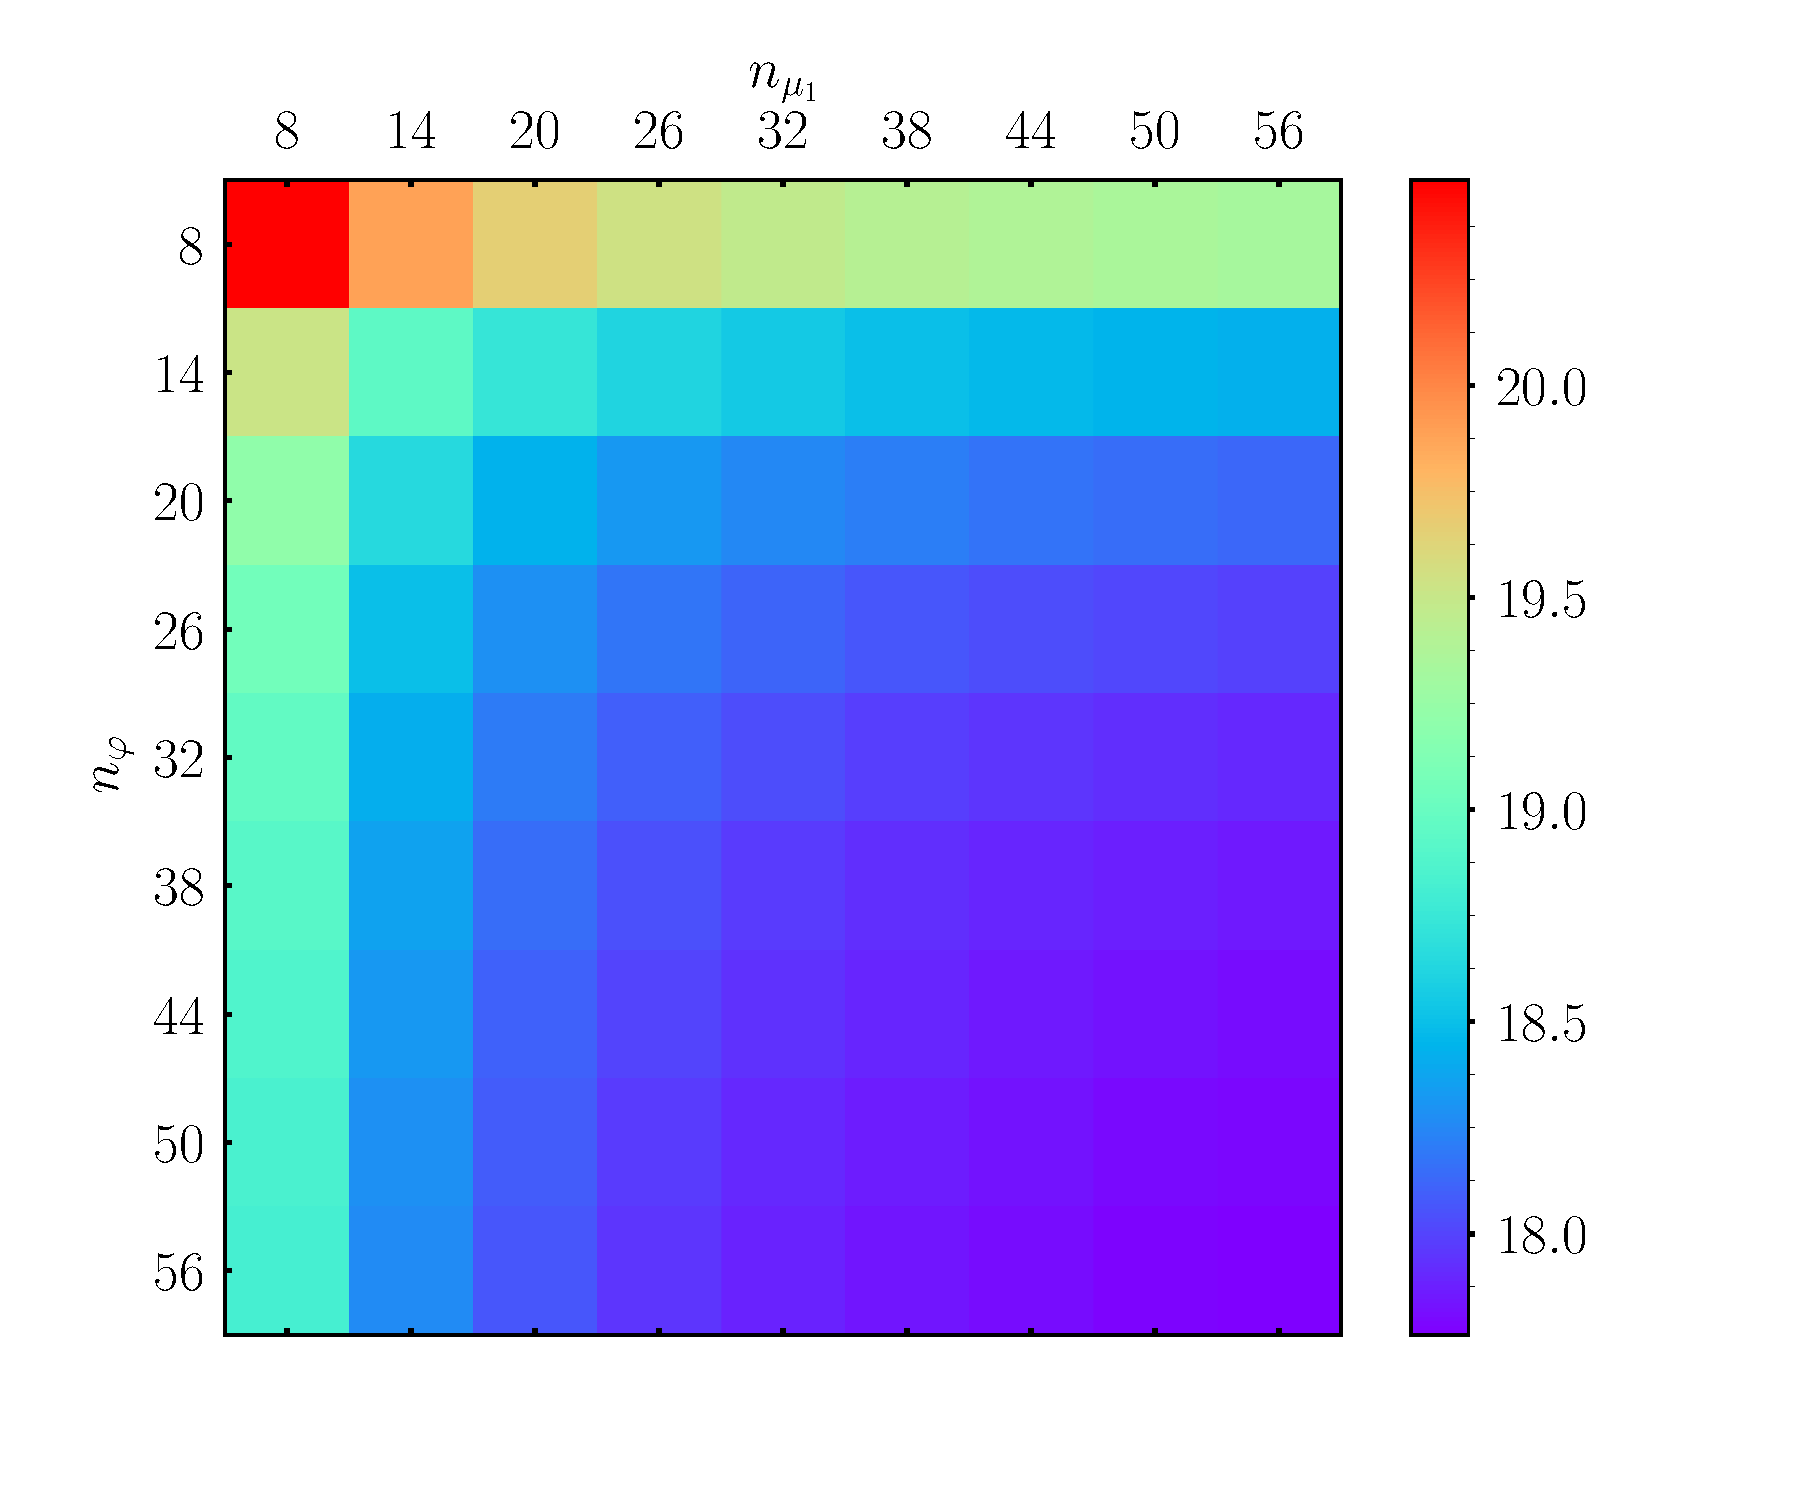
\includegraphics[width=8.0cm]{fig/colournmu1nphi_Doppler-eps-converted-to} 
\caption{Effect on 
{total} relativistic SNR of changing number of  $\varphi$ and $\mu_1$ bins. 
} \label{fig4x}
\end{figure} 


\subsection*{{Effect of changing magnification and evolution biases}}

The effect on the relativistic SNR of changes in magnification bias and in evolution bias is illustrated in Fig.~\ref{fig1x}.

\begin{figure}[ht]
\centering
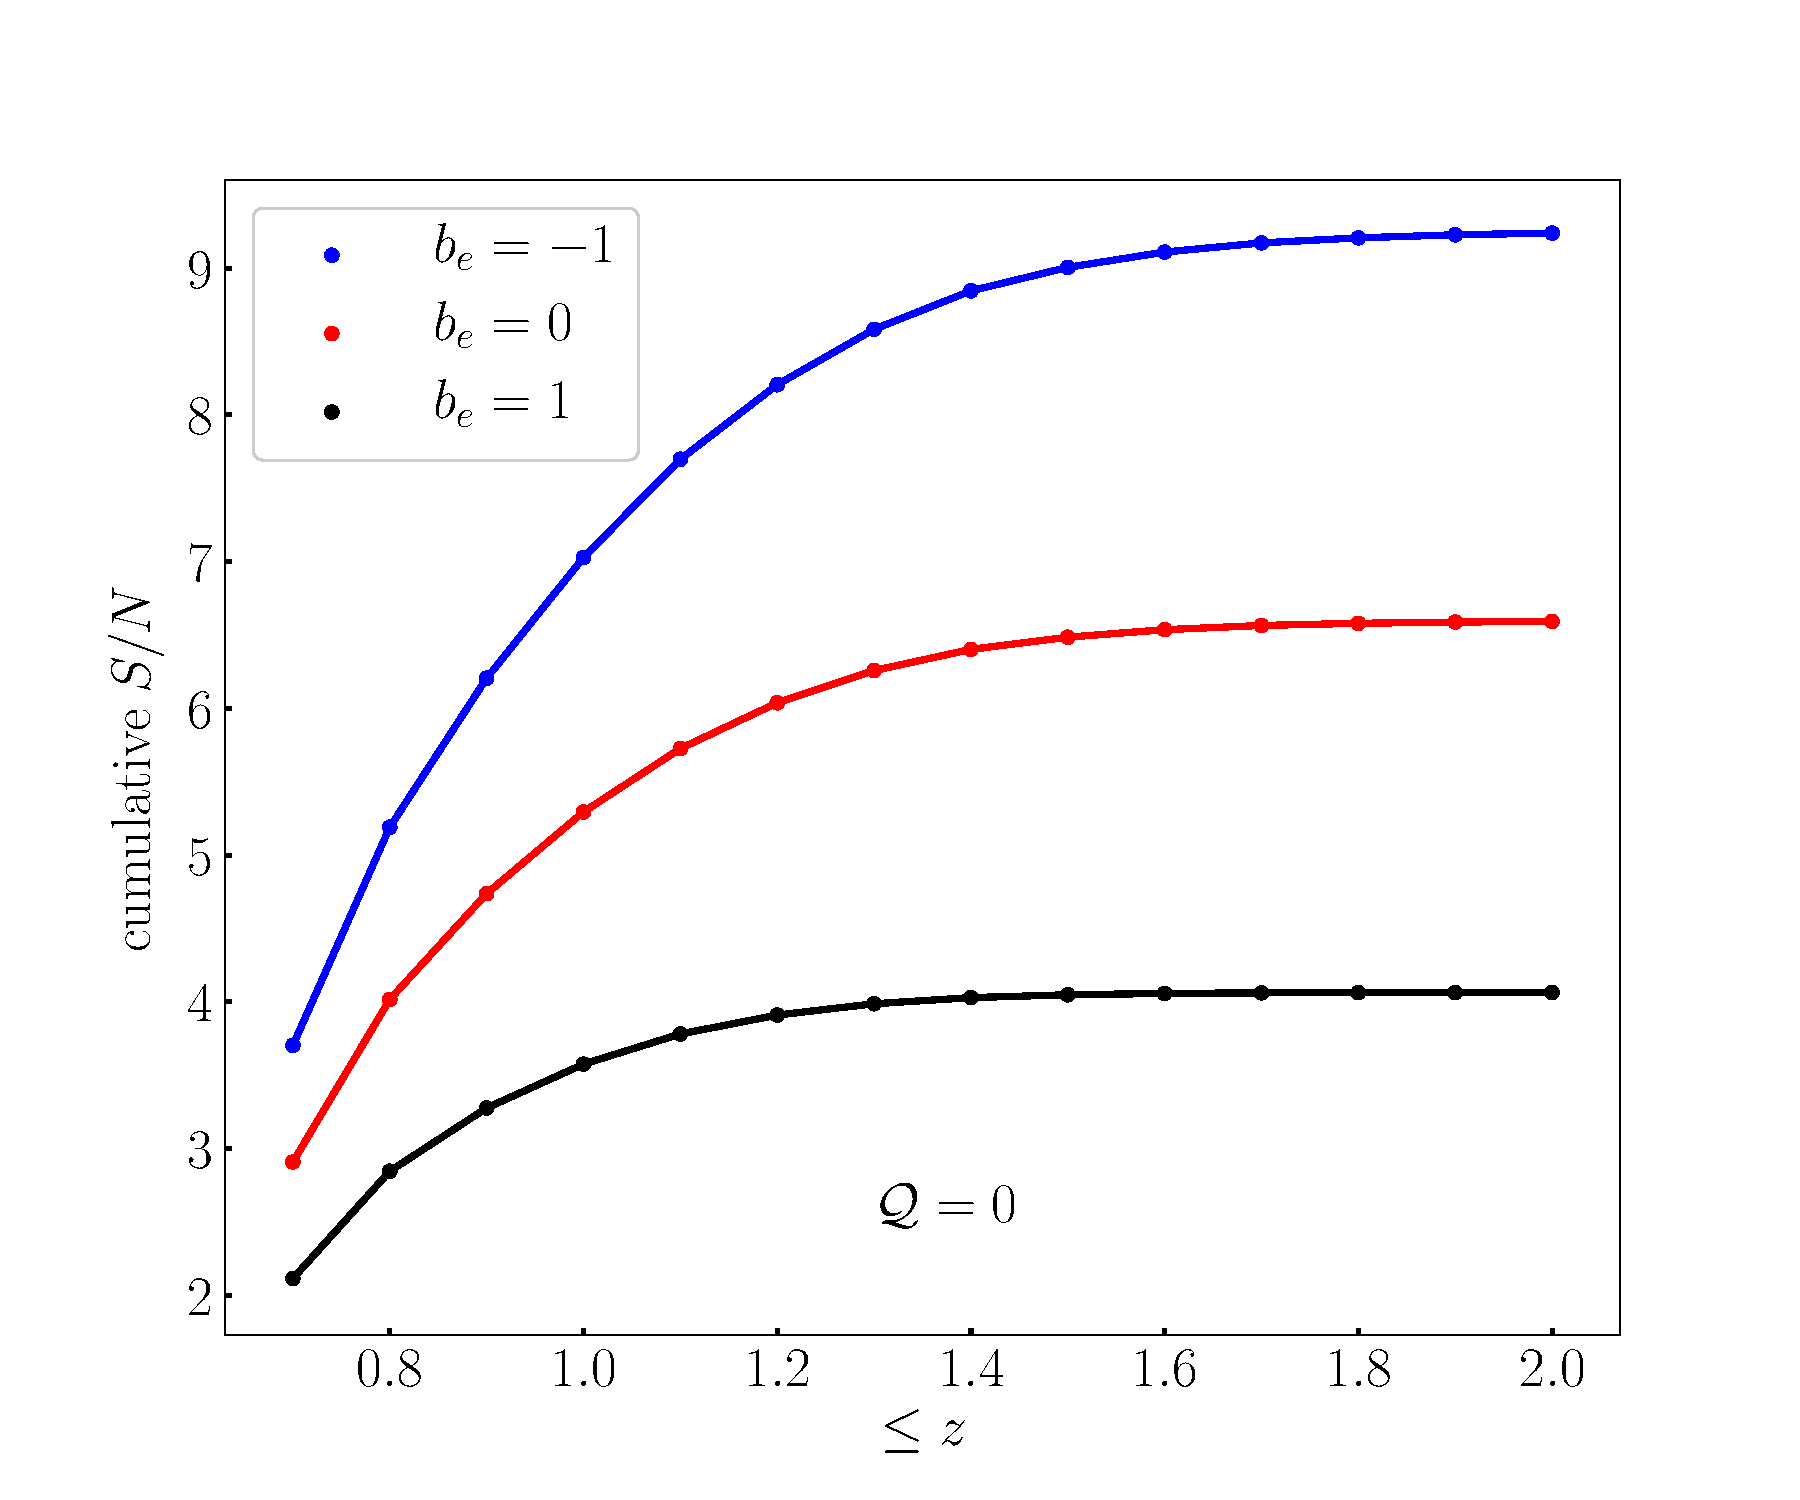
\includegraphics[width=7cm]{fig/cumulativeSnrdopplerQ0_0-eps-converted-to} 
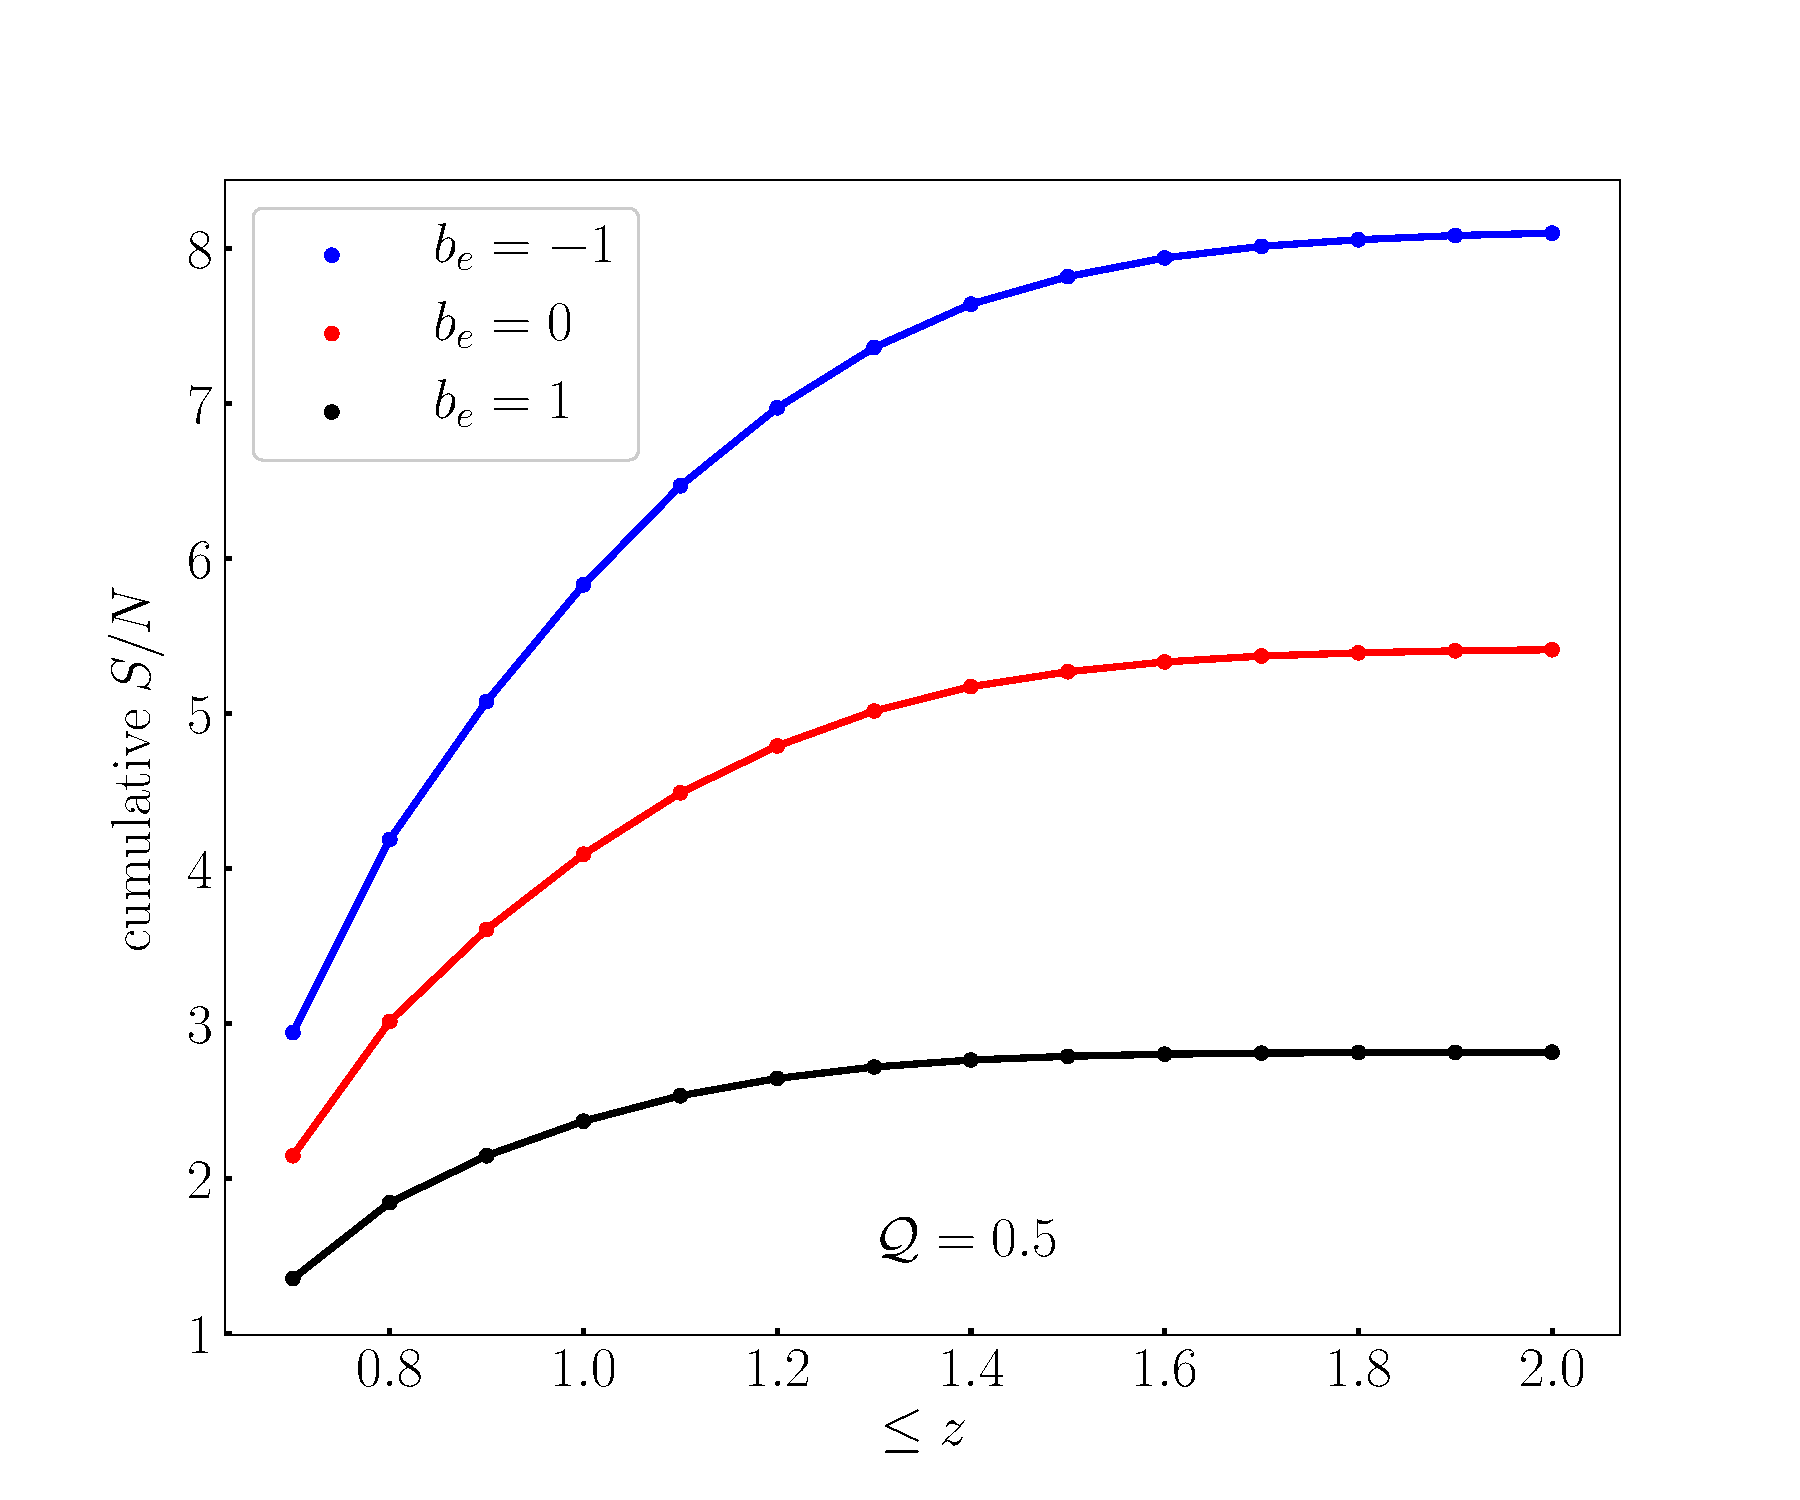
\includegraphics[width=7cm]{fig/cumulativeSnrdopplerQ0_5-eps-converted-to} \\
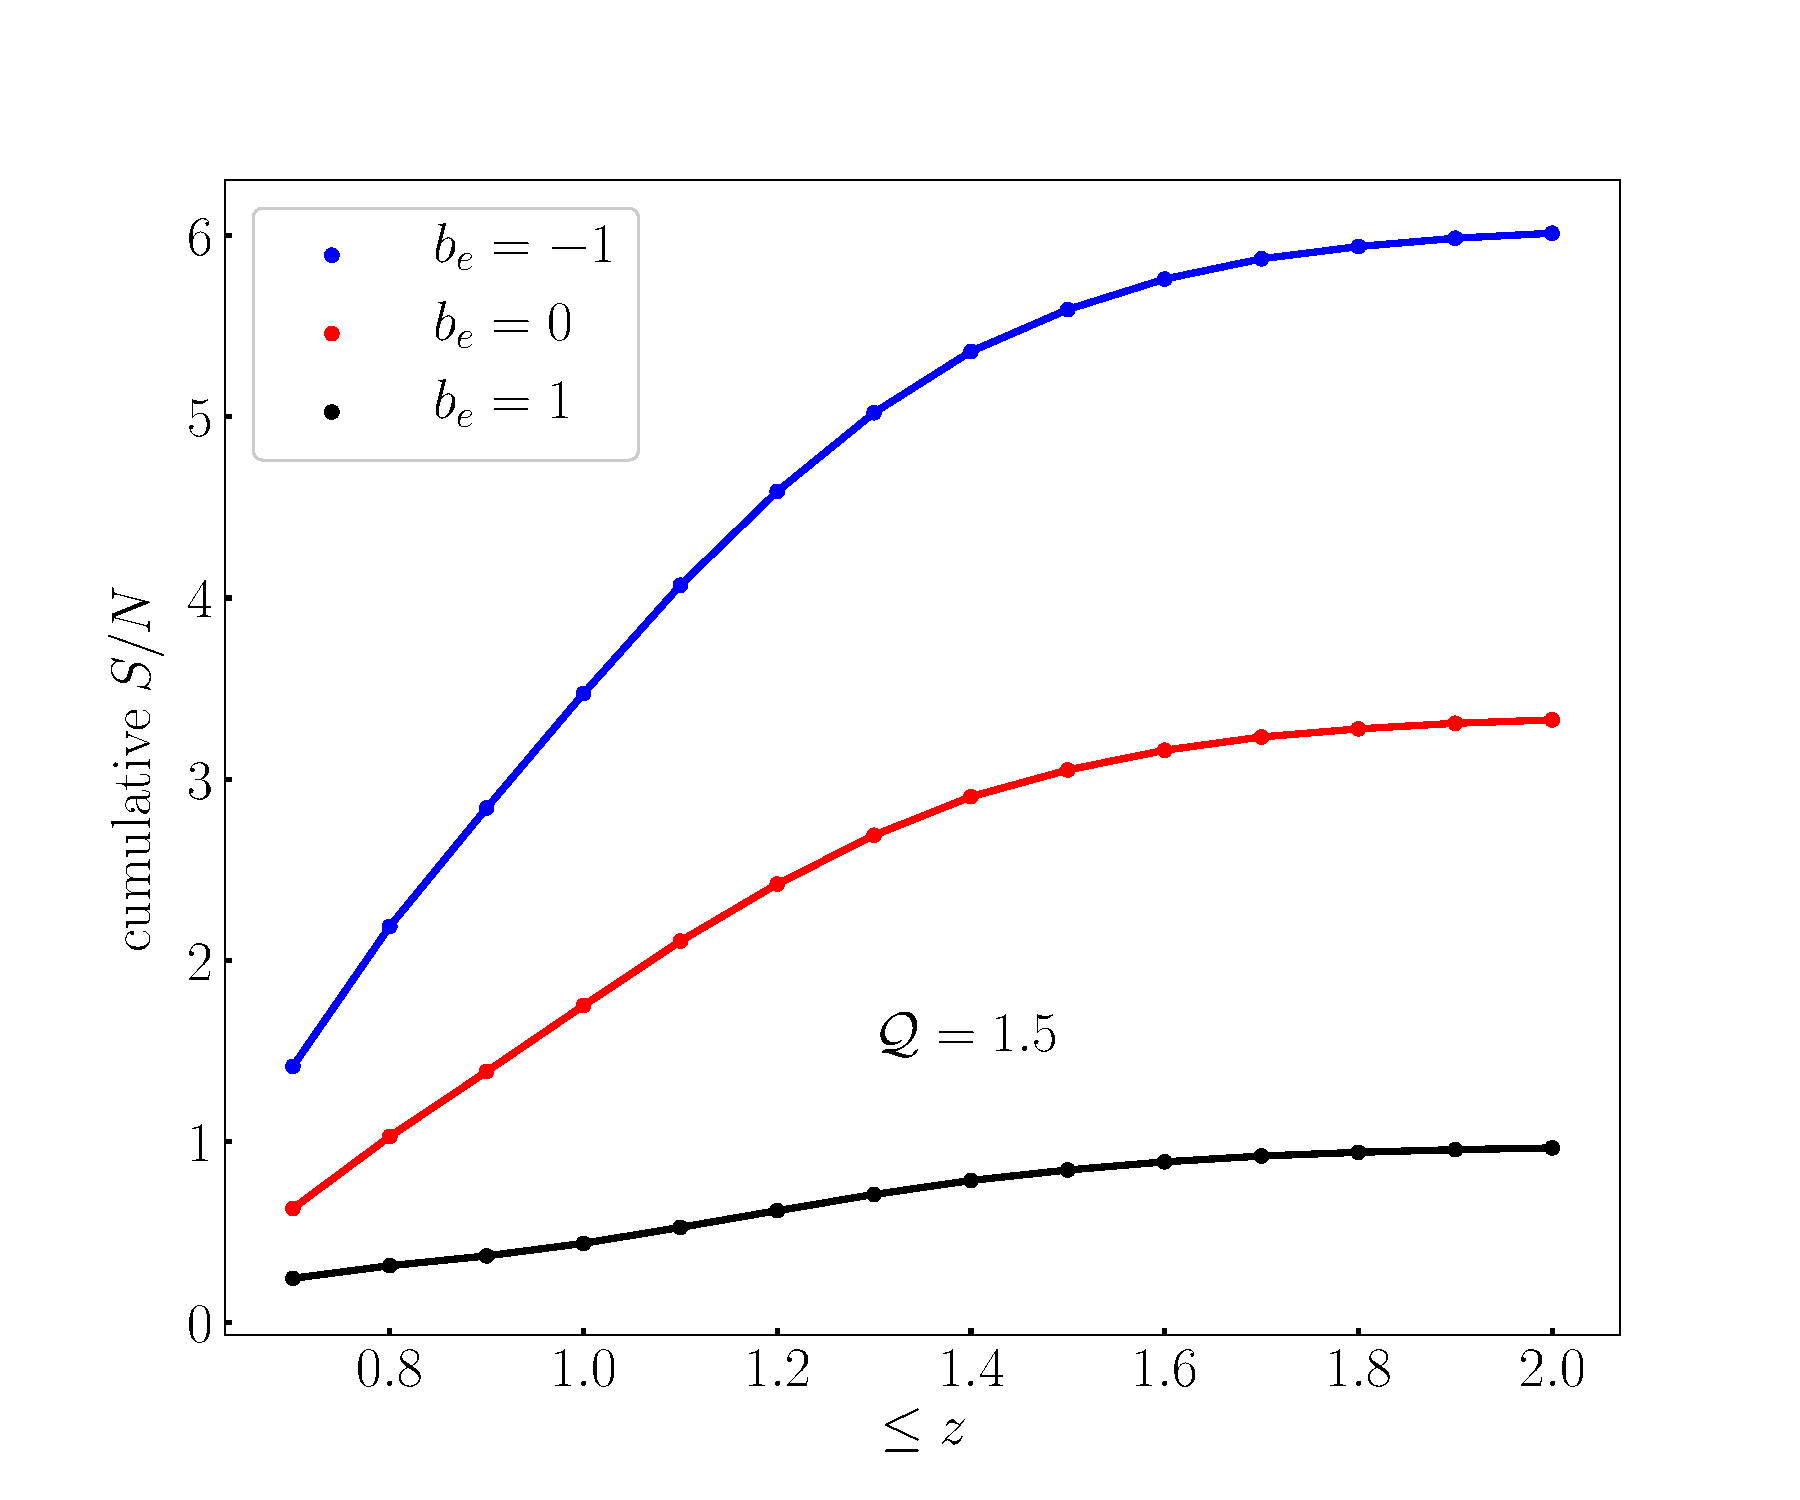
\includegraphics[width=7cm]{fig/cumulativeSnrdopplerQ1_5-eps-converted-to}
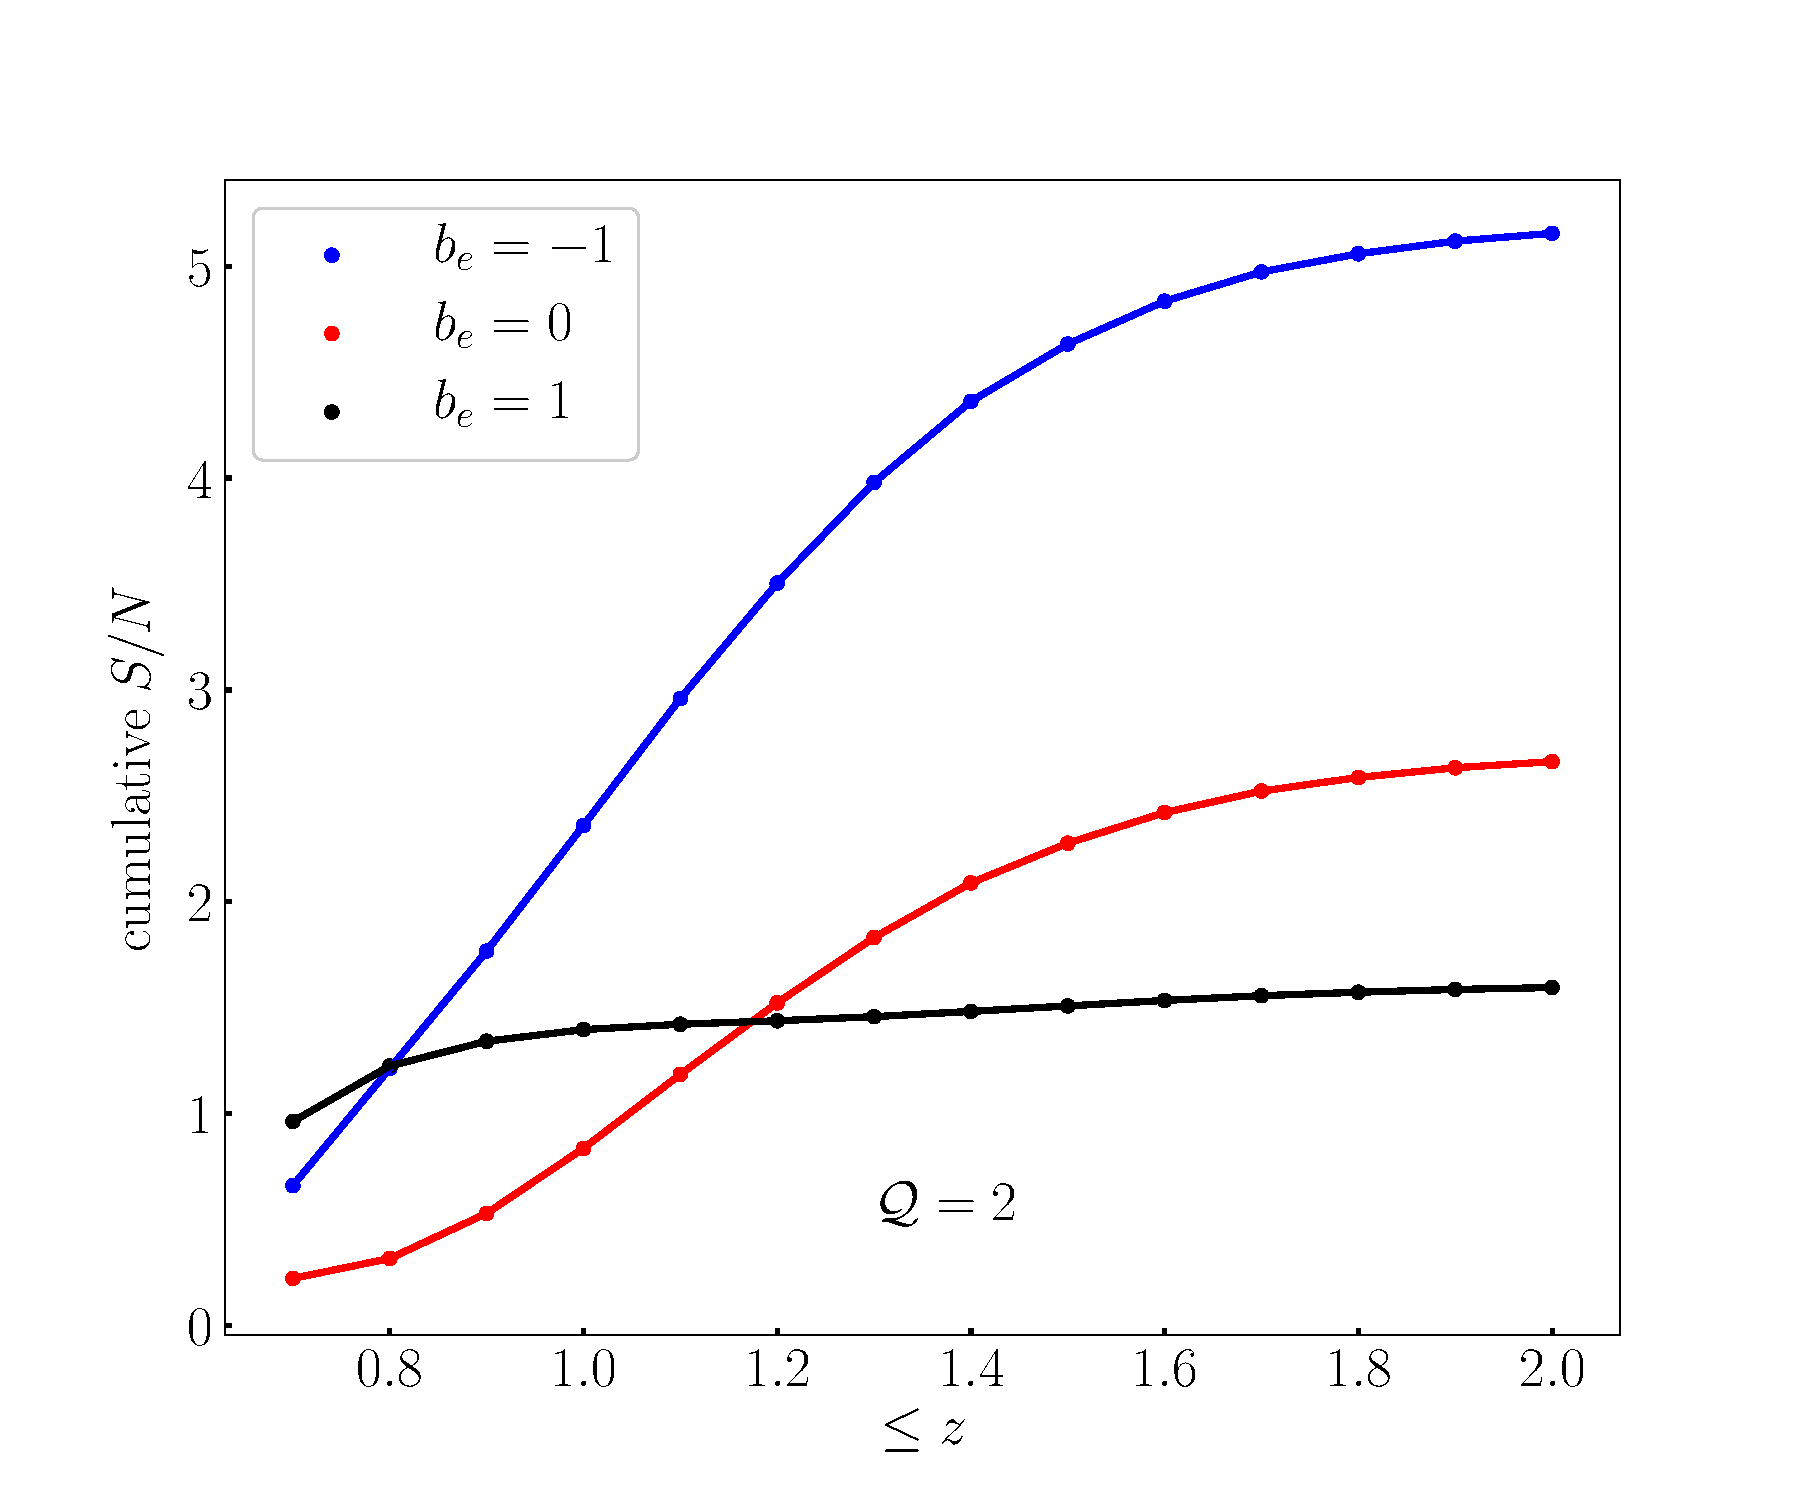
\includegraphics[width=7cm]{fig/cumulativeSnrdopplerQ2_0-eps-converted-to} 
\caption{Effect of changing ${\cal Q}$ and $b_e$ on relativistic cumulative SNR.} \label{fig1x}
\end{figure}


\subsection*{{Comparison with \cite{Jeong:2019igb}}}

In \cite{Jeong:2019igb},  
a significant number of terms is neglected in the relativistic second-order  galaxy number count contrast, $\delta_{g\mathrm{D}}^{(2)}$, given by our \eqref{dg2}. (Note that our  \eqref{dg2}, derived in \cite{Clarkson:2018dwn}, was independently confirmed by \cite{DiDio:2018zmk}). They have the first term, $A\, \bm{v}^{(2)}\!\!\cdot\bm{n}$, on the right of \eqref{dg2}.  In the second term, $2{C}(\bm{v}\cdot\bm{n})\,\delta$, they do not have the correct form of the coefficient $C$ -- they include only the first part, $b_1A$, of $C$ [see the right-hand side of eq 26?]. All terms after the second term in \eqref{dg2} are omitted by \cite{Jeong:2019igb}. Note that none of the omitted terms is suppressed by a higher power of $k^{-1}$;  they all have the same scaling, i.e., $\propto (\cH/k)\,{(\delta)^2}$. In detail, they omit the following
terms:
\begin{align}
\delta_{g\mathrm{D}}^{(2)}({\mathrm{us}})- \delta_{g\mathrm{D}}^{(2)}(\mbox{{\cite{Jeong:2019igb}}}) &= 2\left[b_{1}f + \frac{b_1'}{\cH} 
+ 2\bigg(1-\frac{1}{{r} \cH}\bigg){\frac{\partial b_1}{\partial \ln{L}}\bigg|_{\mathrm{c}}} \right](\bm{v}\cdot\bm{n})\,\delta 
\\\nonumber
& 
+ \frac{2}{\cH}\left(4-2A-\frac{3}{2}\Omega_{m} \right)(\bm{v}\cdot\bm{n})\,\partial_r(\bm{v}\cdot\bm{n})\\
\nonumber
&
+ \frac{2}{\cH^2}\big[(\bm{v}\cdot\bm{n}) \,\partial_r^2\Phi-\Phi\, \partial_r^2 (\bm{v}\cdot\bm{n}) \big]
 - \frac{2}{\cH}\,\partial_r (\bm{v}\cdot\bm{v}) + 2 \frac{b_1}{\cH}\,\Phi\, \partial_r\delta \,. 
\end{align}
%
% \chapter{HI intensity mapping}
% \label{app_im}
% %
% \section{HI bias parameters} \label{app1}

We follow \cite{Umeh:2015gza} to compute $b_{1}$ and $b_{2}$ from a halo-model approach:
\begin{align}
b_{1} &= 1 + \left\langle \frac{2p+\big(q\nu - 1\big)\big[1+(q\nu)^{p}\big]}{\delta_{\rm cr}\big[1+(q\nu)^{p}\big]} \right\rangle _{\!\!\!\rm m}  \!\!, \label{e1.16} \\
b_{2} &= \frac{8}{21}\big(b_{1}-1\big) + \left \langle \frac{2p\big(2p+2\nu q-1\big)+ q\nu\big(q\nu-3\big)\big[1+(q\nu)^{p}\big]}{\delta_{\rm cr}^{2}\big[1+(q\nu)^{p}\big]}  \right \rangle _{\!\!\!\rm m}  \!\!, \label{e1.17}
\end{align}
where the parameters $p$, $q$ and $\nu$ are related to the Sheth-Tormen distribution function (see \cite{Sheth:1999su, Sheth:2001dp, Sheth:1999mn} for more details), and $\delta_{\rm cr}$ is the critical density at which halos collapse spherically \cite{Kitayama:1996ne}, 
\begin{equation}
\delta_{\rm c}(z) = \frac{3(12\pi)^{2/3}}{20}\big[1+0.0123\log{\Omega_{\rm m} (z)}\big] \,. \label{e1.20}
\end{equation}
The mass average is defined by 
\begin{equation}
\big\langle X_{h}(z,\bm{x}) \big\rangle _{\rm m}  = \frac{\int_{M_{-}}^{M_{+}} \ud M\,X_{h}(z,\bm{x},M)\,M_{\mathrm{HI}}(M)\,n_{h}(z,\bm{x},M)}{\int_{M_{-}}^{M_{+}} \ud M\,M_{\mathrm{HI}}(M)\,n_{h}(z,\bm{x},M)} \, , \label{e1.18}
\end{equation}
where $M$ is the mass of {halos} that can host HI gas, and $M_{\pm}$ are the lower and upper mass limits, which are  related to the circular velocities  of the galaxies \citep{Bull:2014rha}. $n_{h}$ is the halo mass function \citep{Sheth:1999su, Sheth:2001dp,Tellarini:2015faa}, and $M_{\rm HI}$ is the HI mass function, which is assumed to follow a power law  \citep{Santos:2015gra},
\begin{equation}
M_{\mathrm{HI}}(M) \propto M^{0.6} \,. \label{e1.19}
\end{equation}
 Figure~\ref{fig1} shows the numerical results from \eqref{e1.16} and \eqref{e1.17}. Fitting formulas for the bias parameters are
\bea
b_{1}(z)& = & 0.754 + 0.0877z + 0.0607z^{2} - 0.00274z^{3}\,, \label{e1.27} \\
b_{2}(z) &= & -0.308 - 0.0724z - 0.0534z^{2} + 0.0247z^{3}\,. \label{e1.28}
\eea
Assuming that  halo formation is a local process in Lagrangian space and that there is no initial tidal bias, the tidal bias is \cite{Tellarini:2015faa}:
\begin{equation}
b_{s^{2}} = \frac{4}{7}\big(1-b_{1}\big)\,.\label{e1.21} 
\end{equation} 

\clearpage

\section{MeerKAT and SKA system temperatures} \label{app2}
\vspace*{-0.5cm}
\begin{table}[! ht]
\centering
\caption{\label{tab5} System temperatures for MeerKAT and SKA1-MID, used in Figure~\ref{fig2} (from \cite{Fonseca:2019qek}).} 
\vspace*{0.2cm}
  \begin{tabular}{|l|l|l|l|l|l|l|l|}
    \hline
      \multicolumn{2}{|c|}{MeerKAT L Band} &
      \multicolumn{2}{c|}{MeerKAT UHF Band} &
      \multicolumn{2}{c|}{SKA1-MID Band 1} & 
      \multicolumn{2}{c|}{SKA1-MID Band 2} \\
      \hline \hline
    $~~~~z~~$ & $~~T_{\rm sys}\;/\;\rm K~~~$ & $~~~z~$ & $~~~~T_{\rm sys}\;/\;\rm K~~$ & $~~~z~$ & $~~T_{\rm sys}\;/\;\rm K~~$ & $~~~~z~~$ & $~~T_{\rm sys}\;/\;\rm K~~$ \\
    \hline
    
  %& & & & & & & \\
  
     0.136 & ~~~~19.2 & 0.420 & ~~~~~~20.3 & 0.403 & ~~~~27.2 & 0.115 & ~~~~16.4 \\
    
     0.183 & ~~~~19.7 & 0.495 & ~~~~~~21.0 & 0.470 & ~~~~26.9 & 0.168 & ~~~~16.6 \\
    
     0.235 & ~~~~20.3 & 0.578 & ~~~~~~21.7 & 0.539 & ~~~~26.8 & 0.223 & ~~~~16.8 \\
    
     0.291 & ~~~~20.9 & 0.671 & ~~~~~~22.5 & 0.612 & ~~~~26.9 & 0.280 & ~~~~17.0 \\
    
     0.352 & ~~~~21.5 & 0.775 & ~~~~~~23.5 & 0.767 & ~~~~27.5 & 0.341 & ~~~~17.2 \\
    
    0.420 & ~~~~22.3 & 0.893 & ~~~~~~24.7  & 0.850 & ~~~~28.1 & 0.403 & ~~~~17.6 \\
    
    0.495 & ~~~~23.1 & 1.03 & ~~~~~~26.1   & 0.938 & ~~~~28.8 & 0.470  & ~~~~18.0 \\
    
    0.578 & ~~~~24.0 & 1.18 & ~~~~~~27.9   & 1.03  & ~~~~29.8 &        &  \\
    
          &          & 1.37 & ~~~~~~30.3   & 1.12  & ~~~~30.8 &        &  \\
     
          &          & 1.45 & ~~~~~~31.5   & 1.22  & ~~~~32.1 &        &  \\
    
          &          &      &              & 1.33  & ~~~~33.5 &        &   \\
    
          &          &      &              & 1.44  & ~~~~35.2 &        &    \\
    
          &          &      &              & 1.55  & ~~~~37.1 &        &   \\
    
          &          &      &              & 1.67  & ~~~~39.2 &        &   \\
    
          &          &      &              & 1.80  & ~~~~41.6 &        & \\
    
          &          &      &              & 1.93  & ~~~~44.2 &        &  \\
    
          &          &      &              & 2.07  & ~~~~47.2 &        &  \\
    
          &          &      &              & 2.22  & ~~~~50.6 &        &  \\
    
          &          &      &              & 2.37  & ~~~~54.4 &        &  \\
    
          &          &      &              & 2.54  & ~~~~58.6 &        &  \\
    
          &          &      &              & 2.69  & ~~~~63.4 &        &  \\
    
          &          &      &              & 2.87  & ~~~~68.8 &        &  \\
    
          &          &      &              & 3.05  & ~~~~74.8 &        &  \\
    
 %         &          &      &              &       &          &        &  \\
    \hline
  \end{tabular}
\end{table}
\vspace*{-0.5cm}
 \begin{figure}[! h]
\centering
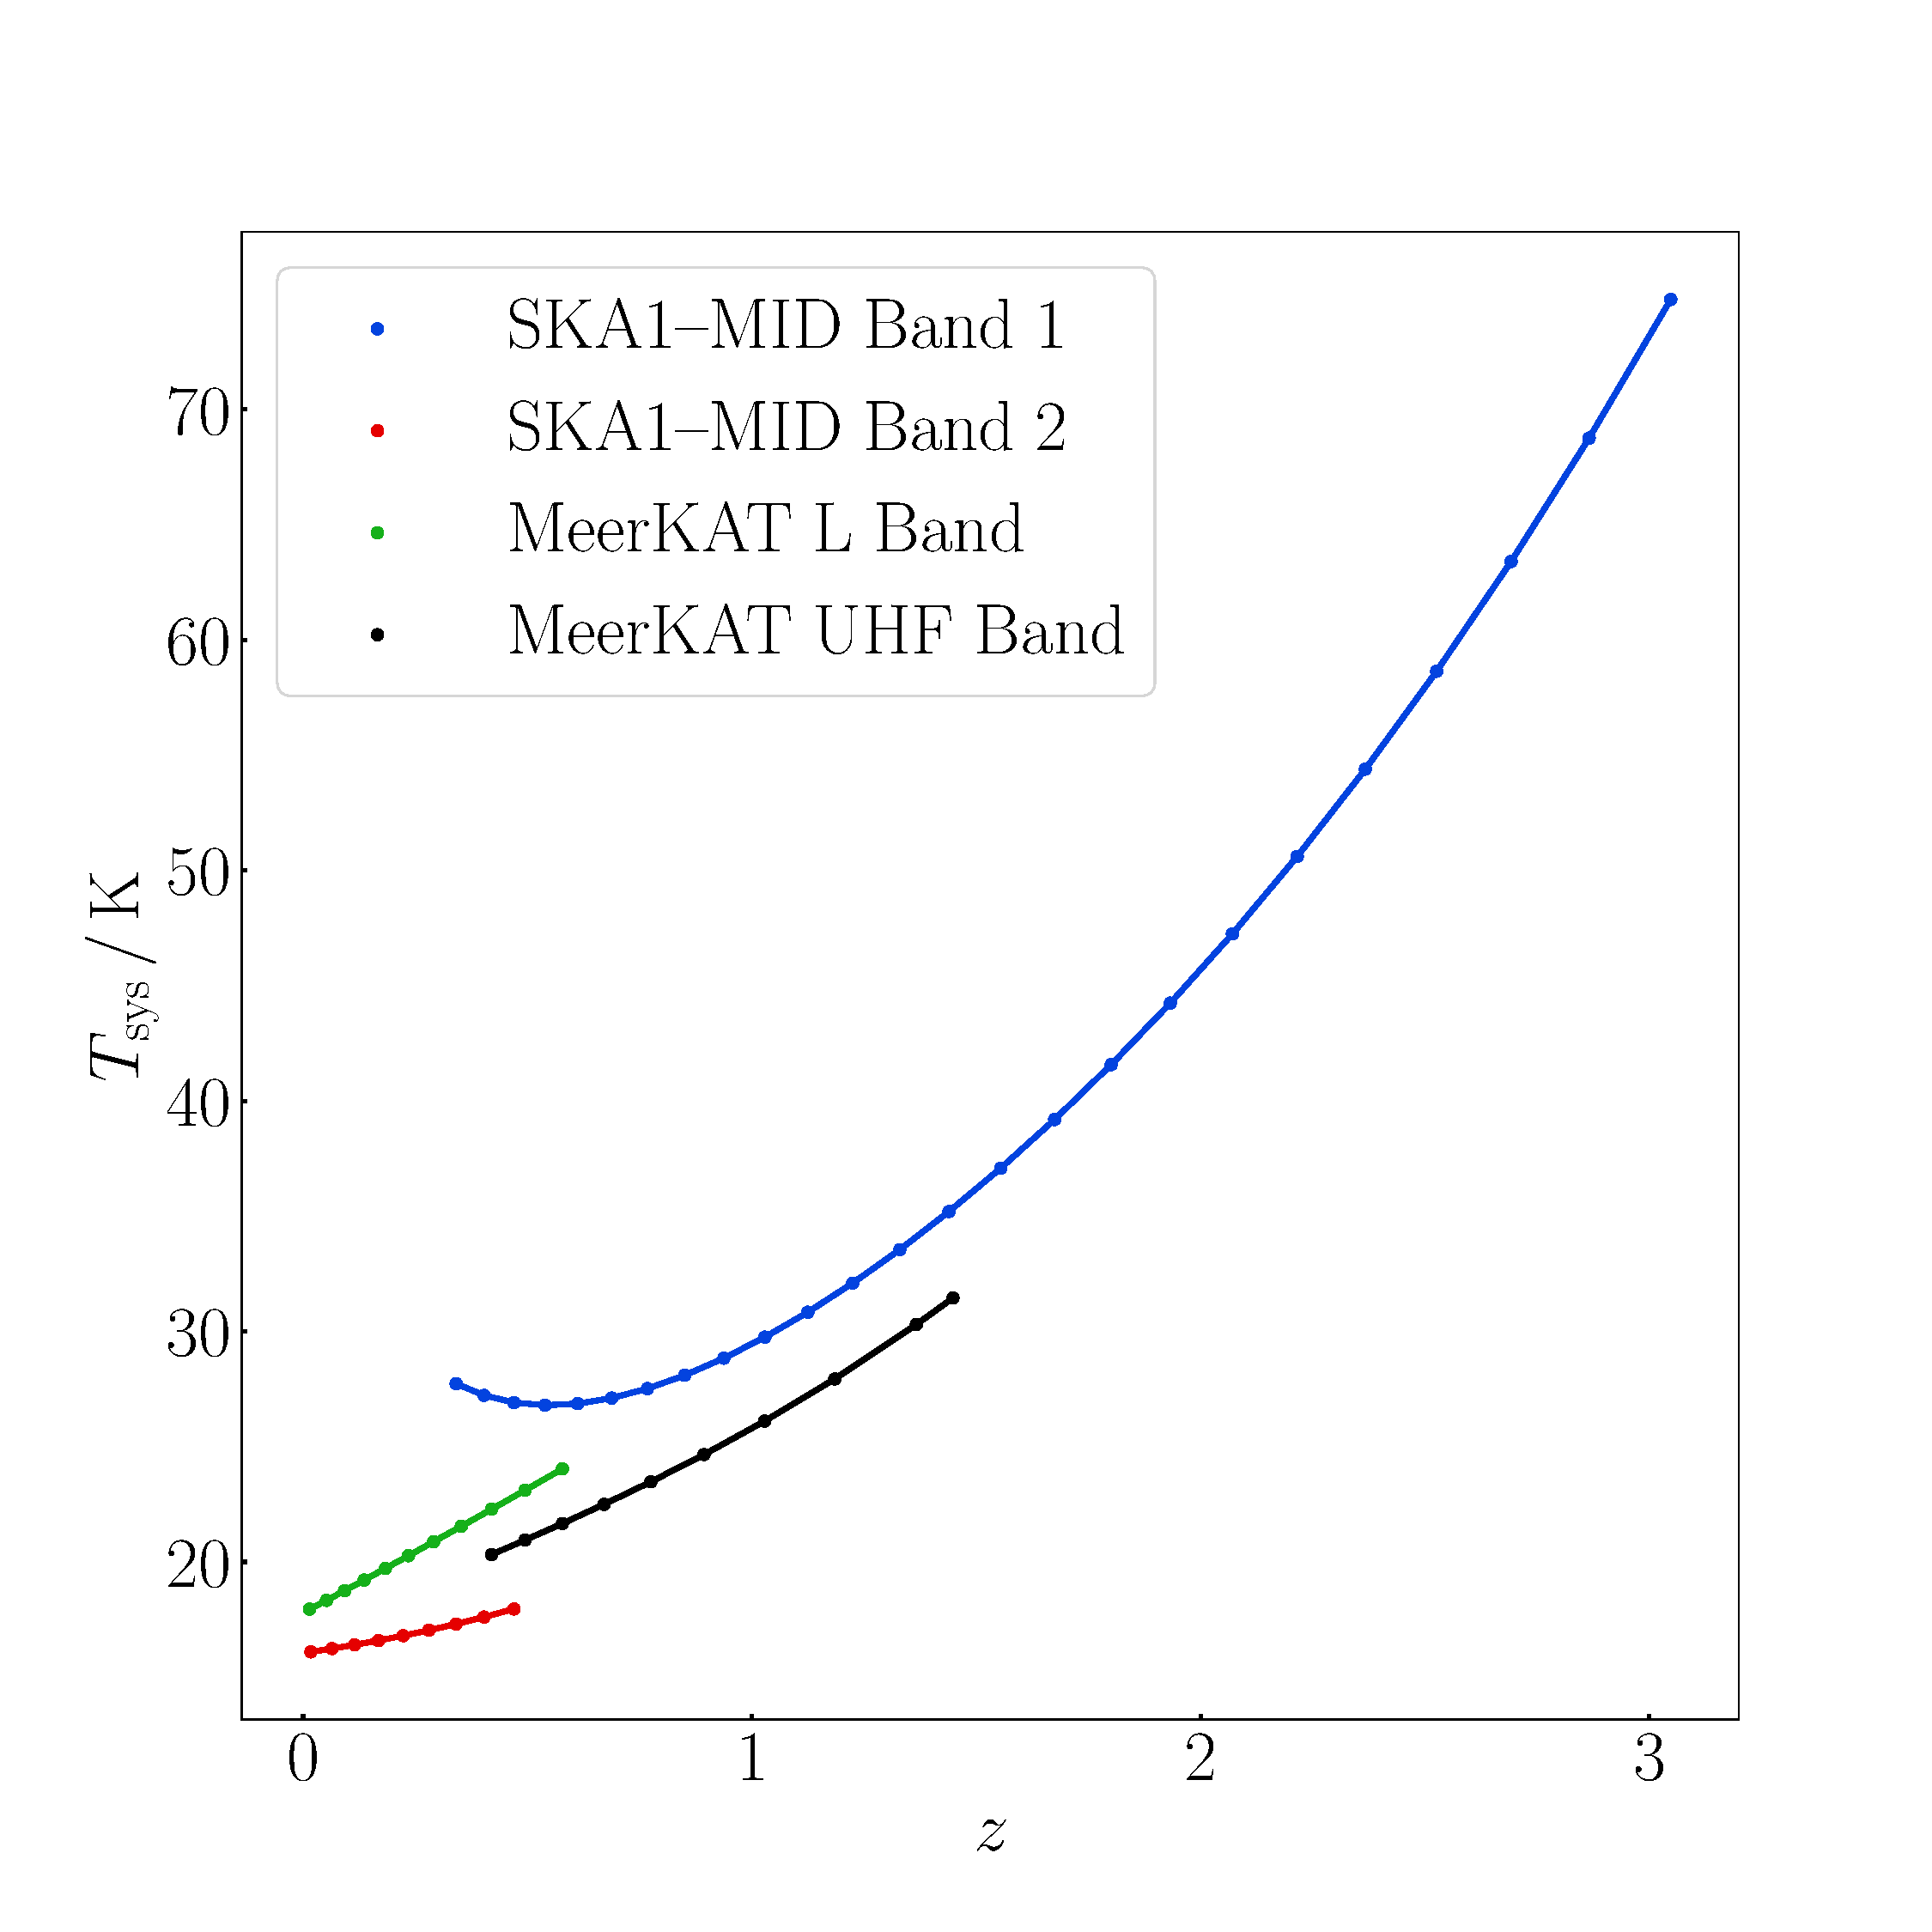
\includegraphics[width=.49\textwidth]{tSys}
\vspace*{-0.5cm}
\caption{$T_{\rm sys}$ for the different frequency bands of MeerKAT and SKA1 (from Table \ref{tab5}).} \label{fig2}
\end{figure}
%
\end{appendices}


% % % % % % % % % % % % % % % % % % % % % % % % % % 
% Start single space again for bibliography
\begin{singlespace}
% % % % % % % % % % % % % % % % % % % % % % % % % 

% Bibliography
% Put your bibliography file here
\bibliography{bib/thesis_bib}
% 
% This bibtex style file puts entries in alphabetical order and treats arxiv
% references correctly.
%\bibliographystyle{abbrvnat}
%\bibliographystyle{unsrt}
%\bibliographystyle{./utphys-ih}
%\bibliographystyle{ieeetr} %cth one I found in order of appearence
%\bibliographystyle{plainnat}


% % % % % % % % % % % % % % % % % % % % % % % % % 

\end{singlespace}

\listoffigures 
\listoftables 


% % % % % % % % % % % % % % % % % % % % % % % % % 
\end{document}
